\documentclass[format=sigconf,natbib=false]{acmart}

\pdfpagewidth 8.5in
\pdfpageheight 11.0in

\usepackage[immediate]{silence}
\WarningFilter{biblatex}{Patching footnotes failed}
\WarningFilter{relsize}{Failed to get list of font sizes}
\usepackage[utf8]{inputenc}
\usepackage[american]{babel}
\usepackage{csquotes}
\usepackage{graphicx}
\usepackage{paralist}
\usepackage{xcolor}
\usepackage{caption,subcaption}
\usepackage{nicefrac}
\usepackage[locale=US]{siunitx}
\usepackage{algorithm,algorithmicx}
\usepackage{algpseudocode}
\usepackage{multirow,bigdelim}
\usepackage{relsize}
\usepackage{booktabs} % For formal tables
\usepackage{tabularx}
\usepackage{cleveref}
\usepackage{hyphenat}
\usepackage{etoolbox}
\usepackage{fmtcount,refcount}
\usepackage{colortbl}
\usepackage{bm}
\usepackage{listings}
\usepackage{biblatex}
\lstset{identifierstyle=\color{black},
	literate={~} {$\sim\,$}{1},
	emph={__global__,__device__},
	emphstyle=\textbf,
	upquote=true,
	showstringspaces=false,
	language=C++,
	columns=fullflexible,
	keepspaces=true,
	basicstyle=\ttfamily,
	keywordstyle=\color{black}\ttfamily\bf,
	stringstyle=\color{red}\ttfamily,
	commentstyle=\color[rgb]{0.4,0.4,0.4}\ttfamily,
	morecomment=[l][\color{magenta}]{\#}
	morekeywords={uint, uint32, uint64, uintll, float4, blockIdx, blockDim, threadIdx},
	numbers=left, 
	numberstyle=\small\color{gray}, 
%                 breaklines=true,
	numbersep=5pt,
	xleftmargin=.19in,
	belowskip=-1.5em
}

\usepackage{tikz}
\usetikzlibrary{arrows.meta}
\usetikzlibrary{matrix}
\usetikzlibrary{shapes}
\usetikzlibrary{decorations.pathreplacing}
\usetikzlibrary{positioning}
\makeatletter
\tikzset{reset label anchor/.code={%
    \let\tikz@auto@anchor=\pgfutil@empty
    \def\tikz@anchor{#1}
  },
  reset label anchor/.default=center
}
\makeatother

% Copyright
%\setcopyright{none}
%\setcopyright{acmcopyright}
%\setcopyright{acmlicensed}
%\setcopyright{rightsretained}
%\setcopyright{usgov}
%\setcopyright{usgovmixed}
%\setcopyright{cagov}
%\setcopyright{cagovmixed}

\copyrightyear{2018} 
\acmYear{2018} 
\setcopyright{acmcopyright}
\acmConference[SIGMOD'18]{2018 International Conference on Management of Data}{June 10--15, 2018}{Houston, TX, USA}
%\acmBooktitle{SIGMOD/PODS '18: 2018 International Conference on Management of Data, June 10--15, 2018, Houston, TX, USA}
\acmPrice{15.00}
\acmDOI{10.1145/3183713.3183740}
\acmISBN{978-1-4503-4703-7/18/06}

\fancyhead{}

\providecommand\={}
\renewcommand{\=}[1][]{\hyp{}#1}

\newtheorem{Definition}{Definition}%[section]
\newcommand{\myequiv}[1]{\ensuremath{\mathrel{\overset{\makebox[0pt]{\mbox{\tiny\sffamily #1}}}{\equiv}}}}

\renewcommand*{\algorithmicrequire}{\textbf{Input:}}
\renewcommand*{\algorithmicensure}{\textbf{Output:}}
\algnewcommand\algorithmicforeach{\textbf{for each}}
\algdef{S}[FOR]{ForEach}[1]{\algorithmicforeach\ #1\ \algorithmicdo}
\algnewcommand{\BitAnd}{\mathrel{\&}}
\algnewcommand{\BitOr}{\mathrel{|}}
\algnewcommand{\BitXor}{\oplus}
\algnewcommand{\ShiftLeft}{\ll}
\algnewcommand{\ShiftRight}{\gg}
\algnewcommand{\BitNeg}{\ensuremath{\mathord{\sim}}}
\algnewcommand{\MB}{\mathbb{B}}
\algnewcommand{\MS}{S_A^{k}}
\algnewcommand{\And}{\textbf{~and~}}
\algnewcommand{\Or}{\textbf{~or~}}
\algnewcommand{\bc}{\mathrm{wt}}

\newcommand{\textat}{\makeatletter @ \makeatother}

\bibliography{sigproc}
\addbibresource{sigproc.bib}
\renewcommand*{\bibfont}{\footnotesize}




\begin{document}
\title[AHEAD: On-the-Fly Hardware Error Detection during Query Processing]{AHEAD: Adaptable Data Hardening for On-the-Fly Hardware Error Detection during Database Query Processing}
%\titlenote{Produces the permission block, and  copyright information}
%\subtitle{Extended Abstract}
%\subtitlenote{The full version of the author's guide is available as \texttt{acmart.pdf} document}

\author{Till Kolditz, Dirk Habich, Wolfgang Lehner}
\affiliation{%
	\institution{Database Systems Group}
	\institution{Technische Universit\"at Dresden}
}
\email{[first.last]@tu-dresden.de}
\author{Matthias Werner}
\affiliation{%
	\institution{Center for Information Services and High Performance Comp.}
	\institution{Technische Universit\"at Dresden}
}
\email{matthias.werner1@tu-dresden.de}
\author{S.T.J. de Bruijn}
\affiliation{%
	\institution{NubiloSoft}
	\city{The Netherlands}
}
\email{stefan@nubilosoft.com}
\renewcommand{\shortauthors}{Till Kolditz et al.}



% !TeX encoding = UTF-8
% !TeX root = sigmod2018.tex
% !TeX spellcheck = en_US
\begin{abstract} 
We have already known for a long time that hardware components are not perfect and soft errors in terms of single bit flips happen all the time. Up to now, these single bit flips are mainly addressed in hardware using general-purpose protection techniques. However, recent studies have shown that all future hardware components become less and less reliable in total and multi-bit flips are occurring regularly rather than exceptionally. Additionally, hardware aging effects will lead to error models that change during run-time. Scaling hardware-based protection techniques to cover changing multi-bit flips is possible, but this introduces large performance, chip area, and power overheads, which will become non-affordable in the future. To tackle that, an emerging research direction is employing protection techniques in higher software layers like compilers or applications. The available knowledge at these layers can be efficiently used to specialize and adapt protection techniques. Thus, we propose a novel adaptable and on-the-fly hardware error detection approach called \emph{AHEAD} for database systems in this paper. \emph{AHEAD} provides configurable error detection in an end-to-end fashion and reduces the overhead (storage and computation) compared to other techniques at this level. Our approach uses an arithmetic error coding technique which allows query processing to completely work on hardened data on the one hand. On the other hand, this enables on-the-fly detection during query processing of (i) errors that modify data stored in memory or transferred on an interconnect and (ii) errors induced during computations. Our exhaustive evaluation clearly shows the benefits of our \emph{AHEAD} approach. 
\end{abstract}


%
% The code below should be generated by the tool at
% http://dl.acm.org/ccs.cfm
% Please copy and paste the code instead of the example below. 
%
\begin{CCSXML}
<ccs2012>
<concept>
<concept_id>10002944.10011123.10010577</concept_id>
<concept_desc>General and reference~Reliability</concept_desc>
<concept_significance>500</concept_significance>
</concept>
<concept>
<concept_id>10002951.10002952.10003190.10003194</concept_id>
<concept_desc>Information systems~Record and buffer management</concept_desc>
<concept_significance>500</concept_significance>
</concept>
<concept>
<concept_id>10002951.10002952.10003190.10010840</concept_id>
<concept_desc>Information systems~Main memory engines</concept_desc>
<concept_significance>500</concept_significance>
</concept>
</ccs2012>
\end{CCSXML}

\ccsdesc[500]{General and reference~Reliability}
\ccsdesc[500]{Information systems~Record and buffer management}
\ccsdesc[500]{Information systems~Main memory engines}

\keywords{Reliability, Error Detection, Database Systems, Query Processing}
\maketitle

%\section{Outline}

\subsection{Introduction}
\begin{itemize}
\item very short introduction
\item ansatz: multi bit flips nehmen zu und hardware schafft es nicht mehr, gerade auch mit Blick auf dynamic
\end{itemize}
\subsection{Problem Description}
Frage nach der Intro: Ist das wirklich ein Problem, was wichtig fuer Datenbanken ist --> Das muss hier untermauert werden (Ja, wichtiges Problem)

\subsubsection{Hardware-Level Protection Techniques}

\subsubsection{Software-Level Protection Techniques}

\subsubsection{Conclusion}
\begin{itemize}
	\item hardware-level protection techniques
	\item software-level protection techniques
	\item Challenges form a Database Perspective
\end{itemize}
\subsection{Software-based Coding}
\begin{itemize}
	\item Error Coding in General
	\item Arithmetic Codes
	\item Analysis and Comparison
\end{itemize}
\subsection{Hardened Data Storage}
\subsection{On-the-fly Error Detection}
\subsection{End-to-End Evaluation}
\subsection{Micro Benchmarks}
\subsection{Related Work}
\subsection{Summary and Future Work}
%\clearpage
% !TeX encoding = UTF-8
% !TeX root = sigmod2018.tex
% !TeX spellcheck = en_US

\vspace{-0.3cm}
\section{Introduction}
\label{sec:Introduction}


The key objective of database systems is to reliably manage data, where high query throughput and low query latency are core requirements~\cite{BeckmanReport2016}. To satisfy these requirements, database systems constantly adapt to novel hardware features~\cite{DBLP:journals/cacm/BonczKM08,DBLP:conf/sigmod/BressFT16,DBLP:conf/sigmod/DoKPPPD13,DBLP:journals/pvldb/KarnagelHL17,DBLP:conf/sigmod/LiDSN16,DBLP:conf/sigmod/OukidLNWL16}. In the recent past, we have seen numerous advances, in particular with respect to \emph{memory}, \emph{processing elements}, and \emph{interconnects}~\cite{DBLP:journals/cacm/BorkarC11,DBLP:journals/dt/Henkel17b,DBLP:conf/micro/Pollack99}. Although it has been intensively studied and commonly accepted that hardware error rates increase dramatically with the decrease of the underlying chip structures ~\cite{DBLP:journals/micro/Borkar05,DBLP:conf/dac/HenkelBDGNSTW13,DBLP:conf/mtdt/SpicaM04}, most database system research activities neglected this fact, traditionally focusing on improving performance characteristics exploiting new data structures and efficient algorithms and leaving error detection (and error correction to some extent) to the underlying hardware. Especially for memory, silent data corruption (SDC) as a result of transient bit flips leading to faulty data is mainly detected and corrected at the DRAM and memory-controller layer~\cite{DBLP:conf/mtdt/SpicaM04}. However, since future hardware becomes less reliable~\cite{DBLP:conf/dac/HenkelBDGNSTW13,DBLP:books/daglib/0037372,DBLP:journals/it/ShafiqueABCCDEH15} and error detection as well as correction by hardware becomes more expensive, this free-ride will come to an end in the near future.

The increasing hardware unreliability is already observable. For instance, repeatedly accessing one memory cell in DRAM modules causes bit flips in physi\-cally-adjacent memory cells~\cite{DBLP:conf/isca/KimDKFLLWLM14,DBLP:conf/date/Mutlu17}. The reason for this is a hardware failure mechanism called \emph{disturbance error}~\cite{DBLP:conf/isca/KimDKFLLWLM14,DBLP:conf/date/Mutlu17}, where electromagnetic (cell-to-cell) interference leads to bit flips. It is already known that this interference effect increases with smaller feature sizes and higher densities of transistors~\cite{DBLP:conf/isca/KimDKFLLWLM14,DBLP:conf/date/Mutlu17}. Kim et al.~\cite{DBLP:conf/isca/KimDKFLLWLM14} evaluated that all newer DRAM modules are affected and they observed one to four bit flips per $64$ bit word even for error-correcting code DRAM (ECC DRAM). Other recent studies have also shown that multi-bit flips become more frequent and that the bit flip model changes at run-time due to transistor aging~\cite{DBLP:conf/isca/KimDKFLLWLM14,DBLP:books/daglib/0037372}. Additionally, hardware-based protection is very challenging~\cite{DBLP:conf/dac/HenkelBDGNSTW13,DBLP:books/daglib/0037372,DBLP:journals/it/ShafiqueABCCDEH15}. Thus, the semiconductor as well as hardware/software communities have recently experienced a shift towards mitigating these reliability issues also at higher software layers, rather than completely mitigating these issues in hardware~\cite{DBLP:conf/dac/HenkelBDGNSTW13,DBLP:books/daglib/0037372}.

Consequently, several software-level reliability techniques have evolved, e.g., error detection using duplicated instructions~\cite{oh2002error} or software implemented fault tolerance (SWIFT)~\cite{DBLP:conf/cgo/ReisCVRA05}. These general-purpose software techniques are usually based on data/code redundancy using dual or triple modular redundancy (DMR/TMR). However, the application of these techniques with respect to in-memory database systems causes a high overhead as illustrated in Figure~\ref{fig:teaser}. Obviously, software-based DMR protection requires twice as much memory capacity compared to a normal (unprotected) setting, since data must be kept twice in different main memory locations. Furthermore, every query is redundantly executed with an additional voting at the end resulting in a computational overhead slightly higher than 2x. Figure~\ref{fig:teaser} highlights the average relative overheads for all $13$ queries of the SSB benchmark~\cite{oneil2009ssbm,DBLP:journals/corr/Sanchez16a} with the unprotected approach as baseline.

\begin{figure}[t]
	{
		\footnotesize
		\graphicspath{{results/ssb/}}
		\null
		\begin{subfigure}[t]{1in}
			% GNUPLOT: LaTeX picture with Postscript
\begingroup
  \makeatletter
  \providecommand\color[2][]{%
    \GenericError{(gnuplot) \space\space\space\@spaces}{%
      Package color not loaded in conjunction with
      terminal option `colourtext'%
    }{See the gnuplot documentation for explanation.%
    }{Either use 'blacktext' in gnuplot or load the package
      color.sty in LaTeX.}%
    \renewcommand\color[2][]{}%
  }%
  \providecommand\includegraphics[2][]{%
    \GenericError{(gnuplot) \space\space\space\@spaces}{%
      Package graphicx or graphics not loaded%
    }{See the gnuplot documentation for explanation.%
    }{The gnuplot epslatex terminal needs graphicx.sty or graphics.sty.}%
    \renewcommand\includegraphics[2][]{}%
  }%
  \providecommand\rotatebox[2]{#2}%
  \@ifundefined{ifGPcolor}{%
    \newif\ifGPcolor
    \GPcolortrue
  }{}%
  \@ifundefined{ifGPblacktext}{%
    \newif\ifGPblacktext
    \GPblacktexttrue
  }{}%
  % define a \g@addto@macro without @ in the name:
  \let\gplgaddtomacro\g@addto@macro
  % define empty templates for all commands taking text:
  \gdef\gplbacktext{}%
  \gdef\gplfronttext{}%
  \makeatother
  \ifGPblacktext
    % no textcolor at all
    \def\colorrgb#1{}%
    \def\colorgray#1{}%
  \else
    % gray or color?
    \ifGPcolor
      \def\colorrgb#1{\color[rgb]{#1}}%
      \def\colorgray#1{\color[gray]{#1}}%
      \expandafter\def\csname LTw\endcsname{\color{white}}%
      \expandafter\def\csname LTb\endcsname{\color{black}}%
      \expandafter\def\csname LTa\endcsname{\color{black}}%
      \expandafter\def\csname LT0\endcsname{\color[rgb]{1,0,0}}%
      \expandafter\def\csname LT1\endcsname{\color[rgb]{0,1,0}}%
      \expandafter\def\csname LT2\endcsname{\color[rgb]{0,0,1}}%
      \expandafter\def\csname LT3\endcsname{\color[rgb]{1,0,1}}%
      \expandafter\def\csname LT4\endcsname{\color[rgb]{0,1,1}}%
      \expandafter\def\csname LT5\endcsname{\color[rgb]{1,1,0}}%
      \expandafter\def\csname LT6\endcsname{\color[rgb]{0,0,0}}%
      \expandafter\def\csname LT7\endcsname{\color[rgb]{1,0.3,0}}%
      \expandafter\def\csname LT8\endcsname{\color[rgb]{0.5,0.5,0.5}}%
    \else
      % gray
      \def\colorrgb#1{\color{black}}%
      \def\colorgray#1{\color[gray]{#1}}%
      \expandafter\def\csname LTw\endcsname{\color{white}}%
      \expandafter\def\csname LTb\endcsname{\color{black}}%
      \expandafter\def\csname LTa\endcsname{\color{black}}%
      \expandafter\def\csname LT0\endcsname{\color{black}}%
      \expandafter\def\csname LT1\endcsname{\color{black}}%
      \expandafter\def\csname LT2\endcsname{\color{black}}%
      \expandafter\def\csname LT3\endcsname{\color{black}}%
      \expandafter\def\csname LT4\endcsname{\color{black}}%
      \expandafter\def\csname LT5\endcsname{\color{black}}%
      \expandafter\def\csname LT6\endcsname{\color{black}}%
      \expandafter\def\csname LT7\endcsname{\color{black}}%
      \expandafter\def\csname LT8\endcsname{\color{black}}%
    \fi
  \fi
    \setlength{\unitlength}{0.0500bp}%
    \ifx\gptboxheight\undefined%
      \newlength{\gptboxheight}%
      \newlength{\gptboxwidth}%
      \newsavebox{\gptboxtext}%
    \fi%
    \setlength{\fboxrule}{0.5pt}%
    \setlength{\fboxsep}{1pt}%
\begin{picture}(1440.00,1440.00)%
    \gplgaddtomacro\gplbacktext{%
      \csname LTb\endcsname%
      \put(448,124){\makebox(0,0)[r]{\strut{}\num{0}}}%
      \csname LTb\endcsname%
      \put(448,375){\makebox(0,0)[r]{\strut{}\num{0.5}}}%
      \csname LTb\endcsname%
      \put(448,625){\makebox(0,0)[r]{\strut{}\num{1}}}%
      \csname LTb\endcsname%
      \put(448,876){\makebox(0,0)[r]{\strut{}\num{1.5}}}%
      \csname LTb\endcsname%
      \put(448,1126){\makebox(0,0)[r]{\strut{}\num{2}}}%
      \csname LTb\endcsname%
      \put(448,1377){\makebox(0,0)[r]{\strut{}\num{2.5}}}%
      \csname LTb\endcsname%
      \put(814,751){\makebox(0,0)[l]{\strut{}1}}%
      \csname LTb\endcsname%
      \put(960,1252){\makebox(0,0)[l]{\strut{}2.01}}%
      \csname LTb\endcsname%
      \put(1139,826){\makebox(0,0)[l]{\strut{}1.19}}%
    }%
    \gplgaddtomacro\gplfronttext{%
      \csname LTb\endcsname%
      \put(130,750){\rotatebox{-270}{\makebox(0,0){\strut{}Relative Runtime}}}%
    }%
    \gplbacktext
    \put(0,0){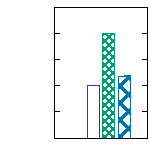
\includegraphics{runtimes}}%
    \gplfronttext
  \end{picture}%
\endgroup

			%\caption{Runtime}
			\caption{Runtime}
			\label{fig:teaser:runtime}%
		\end{subfigure}
		\hfill
		\begin{subfigure}[t]{1in}
			% GNUPLOT: LaTeX picture with Postscript
\begingroup
  \makeatletter
  \providecommand\color[2][]{%
    \GenericError{(gnuplot) \space\space\space\@spaces}{%
      Package color not loaded in conjunction with
      terminal option `colourtext'%
    }{See the gnuplot documentation for explanation.%
    }{Either use 'blacktext' in gnuplot or load the package
      color.sty in LaTeX.}%
    \renewcommand\color[2][]{}%
  }%
  \providecommand\includegraphics[2][]{%
    \GenericError{(gnuplot) \space\space\space\@spaces}{%
      Package graphicx or graphics not loaded%
    }{See the gnuplot documentation for explanation.%
    }{The gnuplot epslatex terminal needs graphicx.sty or graphics.sty.}%
    \renewcommand\includegraphics[2][]{}%
  }%
  \providecommand\rotatebox[2]{#2}%
  \@ifundefined{ifGPcolor}{%
    \newif\ifGPcolor
    \GPcolortrue
  }{}%
  \@ifundefined{ifGPblacktext}{%
    \newif\ifGPblacktext
    \GPblacktexttrue
  }{}%
  % define a \g@addto@macro without @ in the name:
  \let\gplgaddtomacro\g@addto@macro
  % define empty templates for all commands taking text:
  \gdef\gplbacktext{}%
  \gdef\gplfronttext{}%
  \makeatother
  \ifGPblacktext
    % no textcolor at all
    \def\colorrgb#1{}%
    \def\colorgray#1{}%
  \else
    % gray or color?
    \ifGPcolor
      \def\colorrgb#1{\color[rgb]{#1}}%
      \def\colorgray#1{\color[gray]{#1}}%
      \expandafter\def\csname LTw\endcsname{\color{white}}%
      \expandafter\def\csname LTb\endcsname{\color{black}}%
      \expandafter\def\csname LTa\endcsname{\color{black}}%
      \expandafter\def\csname LT0\endcsname{\color[rgb]{1,0,0}}%
      \expandafter\def\csname LT1\endcsname{\color[rgb]{0,1,0}}%
      \expandafter\def\csname LT2\endcsname{\color[rgb]{0,0,1}}%
      \expandafter\def\csname LT3\endcsname{\color[rgb]{1,0,1}}%
      \expandafter\def\csname LT4\endcsname{\color[rgb]{0,1,1}}%
      \expandafter\def\csname LT5\endcsname{\color[rgb]{1,1,0}}%
      \expandafter\def\csname LT6\endcsname{\color[rgb]{0,0,0}}%
      \expandafter\def\csname LT7\endcsname{\color[rgb]{1,0.3,0}}%
      \expandafter\def\csname LT8\endcsname{\color[rgb]{0.5,0.5,0.5}}%
    \else
      % gray
      \def\colorrgb#1{\color{black}}%
      \def\colorgray#1{\color[gray]{#1}}%
      \expandafter\def\csname LTw\endcsname{\color{white}}%
      \expandafter\def\csname LTb\endcsname{\color{black}}%
      \expandafter\def\csname LTa\endcsname{\color{black}}%
      \expandafter\def\csname LT0\endcsname{\color{black}}%
      \expandafter\def\csname LT1\endcsname{\color{black}}%
      \expandafter\def\csname LT2\endcsname{\color{black}}%
      \expandafter\def\csname LT3\endcsname{\color{black}}%
      \expandafter\def\csname LT4\endcsname{\color{black}}%
      \expandafter\def\csname LT5\endcsname{\color{black}}%
      \expandafter\def\csname LT6\endcsname{\color{black}}%
      \expandafter\def\csname LT7\endcsname{\color{black}}%
      \expandafter\def\csname LT8\endcsname{\color{black}}%
    \fi
  \fi
    \setlength{\unitlength}{0.0500bp}%
    \ifx\gptboxheight\undefined%
      \newlength{\gptboxheight}%
      \newlength{\gptboxwidth}%
      \newsavebox{\gptboxtext}%
    \fi%
    \setlength{\fboxrule}{0.5pt}%
    \setlength{\fboxsep}{1pt}%
\begin{picture}(1440.00,1440.00)%
    \gplgaddtomacro\gplbacktext{%
      \csname LTb\endcsname%
      \put(448,124){\makebox(0,0)[r]{\strut{}\num{0}}}%
      \csname LTb\endcsname%
      \put(448,375){\makebox(0,0)[r]{\strut{}\num{0.5}}}%
      \csname LTb\endcsname%
      \put(448,625){\makebox(0,0)[r]{\strut{}\num{1}}}%
      \csname LTb\endcsname%
      \put(448,876){\makebox(0,0)[r]{\strut{}\num{1.5}}}%
      \csname LTb\endcsname%
      \put(448,1126){\makebox(0,0)[r]{\strut{}\num{2}}}%
      \csname LTb\endcsname%
      \put(448,1377){\makebox(0,0)[r]{\strut{}\num{2.5}}}%
      \csname LTb\endcsname%
      \put(814,751){\makebox(0,0)[l]{\strut{}1}}%
      \csname LTb\endcsname%
      \put(960,1252){\makebox(0,0)[l]{\strut{}2.00}}%
      \csname LTb\endcsname%
      \put(1139,1001){\makebox(0,0)[l]{\strut{}1.50}}%
    }%
    \gplgaddtomacro\gplfronttext{%
      \csname LTb\endcsname%
      \put(6,750){\rotatebox{-270}{\makebox(0,0){\strut{}Relative Memory}}}%
      \put(130,750){\rotatebox{-270}{\makebox(0,0){\strut{}Consumption}}}%
    }%
    \gplbacktext
    \put(0,0){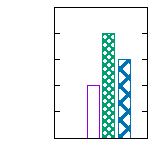
\includegraphics{consumption}}%
    \gplfronttext
  \end{picture}%
\endgroup

			%\caption{Memory Consumption}
			\caption{Storage}
			\label{fig:teaser:memory}%
		\end{subfigure}
		\hfill
		\begin{subfigure}[t]{0.8in}
			% GNUPLOT: LaTeX picture with Postscript
\begingroup
  \makeatletter
  \providecommand\color[2][]{%
    \GenericError{(gnuplot) \space\space\space\@spaces}{%
      Package color not loaded in conjunction with
      terminal option `colourtext'%
    }{See the gnuplot documentation for explanation.%
    }{Either use 'blacktext' in gnuplot or load the package
      color.sty in LaTeX.}%
    \renewcommand\color[2][]{}%
  }%
  \providecommand\includegraphics[2][]{%
    \GenericError{(gnuplot) \space\space\space\@spaces}{%
      Package graphicx or graphics not loaded%
    }{See the gnuplot documentation for explanation.%
    }{The gnuplot epslatex terminal needs graphicx.sty or graphics.sty.}%
    \renewcommand\includegraphics[2][]{}%
  }%
  \providecommand\rotatebox[2]{#2}%
  \@ifundefined{ifGPcolor}{%
    \newif\ifGPcolor
    \GPcolortrue
  }{}%
  \@ifundefined{ifGPblacktext}{%
    \newif\ifGPblacktext
    \GPblacktexttrue
  }{}%
  % define a \g@addto@macro without @ in the name:
  \let\gplgaddtomacro\g@addto@macro
  % define empty templates for all commands taking text:
  \gdef\gplbacktext{}%
  \gdef\gplfronttext{}%
  \makeatother
  \ifGPblacktext
    % no textcolor at all
    \def\colorrgb#1{}%
    \def\colorgray#1{}%
  \else
    % gray or color?
    \ifGPcolor
      \def\colorrgb#1{\color[rgb]{#1}}%
      \def\colorgray#1{\color[gray]{#1}}%
      \expandafter\def\csname LTw\endcsname{\color{white}}%
      \expandafter\def\csname LTb\endcsname{\color{black}}%
      \expandafter\def\csname LTa\endcsname{\color{black}}%
      \expandafter\def\csname LT0\endcsname{\color[rgb]{1,0,0}}%
      \expandafter\def\csname LT1\endcsname{\color[rgb]{0,1,0}}%
      \expandafter\def\csname LT2\endcsname{\color[rgb]{0,0,1}}%
      \expandafter\def\csname LT3\endcsname{\color[rgb]{1,0,1}}%
      \expandafter\def\csname LT4\endcsname{\color[rgb]{0,1,1}}%
      \expandafter\def\csname LT5\endcsname{\color[rgb]{1,1,0}}%
      \expandafter\def\csname LT6\endcsname{\color[rgb]{0,0,0}}%
      \expandafter\def\csname LT7\endcsname{\color[rgb]{1,0.3,0}}%
      \expandafter\def\csname LT8\endcsname{\color[rgb]{0.5,0.5,0.5}}%
    \else
      % gray
      \def\colorrgb#1{\color{black}}%
      \def\colorgray#1{\color[gray]{#1}}%
      \expandafter\def\csname LTw\endcsname{\color{white}}%
      \expandafter\def\csname LTb\endcsname{\color{black}}%
      \expandafter\def\csname LTa\endcsname{\color{black}}%
      \expandafter\def\csname LT0\endcsname{\color{black}}%
      \expandafter\def\csname LT1\endcsname{\color{black}}%
      \expandafter\def\csname LT2\endcsname{\color{black}}%
      \expandafter\def\csname LT3\endcsname{\color{black}}%
      \expandafter\def\csname LT4\endcsname{\color{black}}%
      \expandafter\def\csname LT5\endcsname{\color{black}}%
      \expandafter\def\csname LT6\endcsname{\color{black}}%
      \expandafter\def\csname LT7\endcsname{\color{black}}%
      \expandafter\def\csname LT8\endcsname{\color{black}}%
    \fi
  \fi
    \setlength{\unitlength}{0.0500bp}%
    \ifx\gptboxheight\undefined%
      \newlength{\gptboxheight}%
      \newlength{\gptboxwidth}%
      \newsavebox{\gptboxtext}%
    \fi%
    \setlength{\fboxrule}{0.5pt}%
    \setlength{\fboxsep}{1pt}%
\begin{picture}(1140.00,1440.00)%
    \gplgaddtomacro\gplbacktext{%
    }%
    \gplgaddtomacro\gplfronttext{%
      \csname LTb\endcsname%
      \put(642,1056){\makebox(0,0)[r]{\strut{}Unprotected}}%
      \csname LTb\endcsname%
      \put(642,750){\makebox(0,0)[r]{\strut{}DMR}}%
      \csname LTb\endcsname%
      \put(642,444){\makebox(0,0)[r]{\strut{}AHEAD}}%
    }%
    \gplbacktext
    \put(0,0){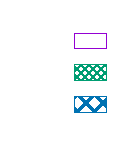
\includegraphics{legend}}%
    \gplfronttext
  \end{picture}%
\endgroup

		\end{subfigure}
		\null
	}
	\vspace{-0.2cm}
%	\caption{Comparing the unprotected in-memory database concept with protected concepts of double modular redundancy (DMR) and our \emph{AHEAD} approach using the star-schema benchmark~\cite{DBLP:journals/corr/Sanchez16a}. More details in Section~\ref{sec:SSBEval}.}
\caption{Relative comparison using the star-schema benchmark~\cite{DBLP:journals/corr/Sanchez16a}. More details in Section~\ref{sec:SSBEval}.}
	\label{fig:teaser}
	\vspace{-0.5cm}
\end{figure}

\textbf{Core Contribution.}
Generally, any undetected bit flip destroys the reliability objective of database systems in form of false negatives (missing tuples), false positives (tuples with invalid predicates) or inaccurate aggregates in a silent way. Since (i) general-purpose software-based protection techniques introduce too much overhead, (ii) memory systems will be significantly more error-prone in the future due to smaller chip structures, and (iii) generic hardware-level detection mechanisms will be too costly and too inflexible, there is a clear need for database-specific approaches to guarantee reliable data storage and processing without sacrificing the overall performance. In this paper, we present a novel approach called \emph{AHEAD} for \textbf{error detection} tailored to state-of-the-art in-memory column store systems~\cite{DBLP:journals/debu/IdreosGNMMK12,DBLP:conf/vldb/StonebrakerABCCFLLMOORTZ05}. As highlighted in Figure~\ref{fig:teaser}, our \emph{AHEAD} approach reduces the overhead compared to DMR to a large degree for storage as well as for processing. Furthermore, multi-bit flips occurring during query processing are on-the-fly detectable, which is not the case for DMR, where errors are only detected during the voting at the end~\cite{DBLP:conf/isca/ReinhardtM00}. We achieve this property and the significant overhead reduction by encoding each value in a fine-grained way using a software-based error coding scheme, which allows to directly work on the encoded data representation during query processing. Moreover, we intentionally devise an \textbf{error detection}-only mechanism and leave the repair mechanism to the database system itself, e.g. by deploying a fine-grained recovery procedure. We intentionally also position our approach \textbf{orthogonal} to other coding domains like compression~\cite{DBLP:conf/sigmod/AbadiMF06} or encryption~\cite{DBLP:journals/sigmod/ShmueliVEG09}, which allows a free combination of different schemes to the underlying data. To represent the intention of detecting hardware errors, we introduce new terms for encoding and decoding. We denote the process of encoding data as \textbf{data hardening}, since data is literally firmed so that corruption becomes detectable. In contrast, we denote as \textbf{data softening} the decoding of data, as it becomes vulnerable to corruption again. Furthermore, we introduce the notion of \textbf{bit flip weight} as the number of flipped bits per logical data value. 


\textbf{Contributions in Detail and Outline.}
To present our novel \emph{AHEAD} approach in detail, we make the following contributions:  
\begin{compactenum}
	\item Reliability concerns for future hardware have attracted major attention in the recent past. In Section~\ref{sec:ProblemEvidence}, we give a precise problem description and define requirements for reliable data management on future hardware.
	\item We promote arithmetic codes as software-based error coding scheme and AN coding as one representative, in Section~\ref{sec:ErrorCoding}. In particular, we justify that AN coding has unique properties with regard to our defined requirements. 	
	\item Based on AN coding, we present our hardened data storage concept for state-of-the-art in-memory column stores in Section~\ref{sec:DataHardening}. Additionally, we describe the adaptation of our hardened storage for various bit flip weights and introduce performance improvements for AN code operations.
	\item Based on this hardened storage foundation, we present our on-the-fly error detection during query processing in Section~\ref{sec:ResilientQueryProcessing}. We introduce different error detection opportunities and determine \emph{continuous detection} as the best solution, for which we describe essential query processing adjustments. 
	\item In Sections~\ref{sec:SSBEval} and~\ref{sec:MicroBenchmarks}, we exhaustively evaluate our \emph{AHEAD} approach, the underlying AN coding scheme, and our developed performance improvements. 
\end{compactenum}
Finally, we present related work in Section~\ref{sec:RelatedWork} as well as briefly summarize the paper including a discussion of future work in Section~\ref{sec:Conclusion}.


%\clearpage
\section{Hardware Reliability Concerns}
\label{sec:ProblemEvidence}

Hardware components fabricated with nano-scale transistors face serious reliability issues like soft errors, aging, thermal hot spots, and process variations as a consequence of the aggressive transistor miniaturization~\cite{DBLP:books/daglib/0037372}. These issues arise from multiple sources and they jeopardize the correct application execution~\cite{DBLP:books/daglib/0037372}. The recently published book~\cite{DBLP:books/daglib/0037372} summarizes state-of-the-art protection techniques in all hardware as well as software layers and presents new results of a large research initiative. In their work, the authors primarily target on soft errors, because soft errors are one of the most important reliability issues in the nano-era. Especially, they describe the technical backgrounds, why soft errors increase with decreasing feature sizes and higher densities of transistors~\cite{DBLP:books/daglib/0037372}.

\textbf{Shift towards Multi-Bit Flips.}
The soft errors are caused due to \emph{external influences} like energetic particle strikes, and/or \emph{internal disruptive events} like noise transients at circuit, chip or system level, cross talks, and electromagnetic interference~\cite{DBLP:books/daglib/0037372}. The soft error rate (SER) grows exponentially, because the number of transistors on the die increases exponentially~\cite{ibe2010impact,DBLP:books/daglib/0037372}. Consequently, multi-bit flips become much more frequent~\cite{DBLP:journals/micro/Borkar05,DBLP:conf/dac/HenkelBDGNSTW13,DBLP:books/daglib/0037372} and transistor aging leads to a changing bit flip behavior at run\=time where heat stimulates this effect~\cite{DBLP:conf/dac/HenkelBDGNSTW13}. All hardware components are affected, but memory cells are more susceptible than logic gates~\cite{DBLP:conf/dac/HenkelBDGNSTW13,DBLP:conf/asplos/HwangSS12,Kim:2007:MET:1331699.1331719}. 

For example, memory technologies are already much more vulnerable to electromagnetic interference effects~\cite{DBLP:conf/isca/KimDKFLLWLM14,DBLP:conf/date/Mutlu17} (\emph{disturbance errors}) as well as to data retention problems. A practical solution to tackle interference effects in DRAM is to increase the DRAM refresh rate, so that the probability of inducing disturbance errors before DRAM cells get refreshed is reduced~\cite{DBLP:conf/isca/KimDKFLLWLM14,DBLP:conf/date/Mutlu17}. However, refresh operations waste energy and degrade system performance by interfering with memory accesses~\cite{DBLP:conf/isca/KimDKFLLWLM14,DBLP:conf/date/Mutlu17}. In addition, with increasing DRAM device capacities, the following effects with regard to DRAM refresh arise at the same time as well (\emph{data retention problem})~\cite{Khan:2014:EEM:2637364.2592000,DBLP:conf/dsn/KhanLM16,Liu:2013:ESD:2508148.2485928,DBLP:conf/date/Mutlu17}. First, more refresh operations are necessary to maintain data correctly. Second, smaller DRAM capacitors require lower retention times~\cite{DBLP:conf/date/Mutlu17}. Third, the voltage margins separating data values become smaller, and as a result the same amount of charge loss is more likely to cause multi-bit flips~\cite{Khan:2014:EEM:2637364.2592000,DBLP:conf/dsn/KhanLM16,Liu:2013:ESD:2508148.2485928,DBLP:conf/date/Mutlu17}. Theses effects increase as DRAM capacities increase~\cite{Khan:2014:EEM:2637364.2592000,DBLP:conf/dsn/KhanLM16,Liu:2013:ESD:2508148.2485928,DBLP:conf/date/Mutlu17}.

Furthermore, emerging non-volatile memory technologies like PCM~\cite{DBLP:conf/isca/LeeIMB09}, STT-MRAM~\cite{DBLP:conf/ispass/KultursayKSM13}, and PRAM~\cite{DBLP:journals/pieee/WongLYCWCLCT12} exhibit similar and perhaps even more reliability issues~\cite{Khan:2014:EEM:2637364.2592000,DBLP:conf/dsn/KhanLM16,Liu:2013:ESD:2508148.2485928,DBLP:conf/date/Mutlu17}. For example, PCM are based on multi-level cells (MLC) to store multiple bits in one cell which is achieved by using intermediate resistive states for storing information, in addition to the low and high resistance levels~\cite{DBLP:journals/computers/Mittal17}. A major problem in PCM is that a time-dependent resistance drift can effect that a different value than the originally stored one will be read~\cite{DBLP:journals/computers/Mittal17}. Furthermore, if one cell drifts to the incorrect state, other cells are also highly likely to drift in the near future. Due to this correlation, multi-bit errors changing at run-time are much more likely in MLC PCM~\cite{DBLP:journals/computers/Mittal17}. Moreover, heat produced by writing one PCM cell can alter the value stored in many nearby cells (e.g., up to $11$ cells in a $64$ byteblock~\cite{DBLP:conf/dsn/JiangZY14})~\cite{DBLP:journals/computers/Mittal17}.

\textbf{Protection Techniques.}
Hardware components usually feature protection techniques such as error correction codes (ECC)~\cite{hamming1950error,Kim:2007:MET:1331699.1331719} or hardware redundancy~\cite{ernst2004razor,su1980hardware}. However, these approaches are aligned to single bit flips nowadays. Thus, hardware research in two directions is necessary: (i) developing appropriate protection technique to cover new effects like \emph{disturbance errors} and/or (ii) scaling up traditional techniques to cover multi\=bit flips. Research is currently done in both directions~\cite{DBLP:books/daglib/0037372}. For example, to mitigate \emph{disturbance errors}, the inter-cell isolation is improved, but this is challenging due to ever-decreasing feature sizes and higher densities~\cite{DBLP:conf/isca/KimDKFLLWLM14,DBLP:conf/date/Mutlu17}. Furthermore, the implementation of multi\=bit error detection and correction codes in memory has been investigated~\cite{Kim:2007:MET:1331699.1331719}. However, this results in high chip area costs for storing the extra parity bits and increased calculation/checking/correction logic, whereas the overhead quickly grows with the code strength~\cite{Kim:2007:MET:1331699.1331719}. Then, reading and computing the parity bits can be a bottleneck~\cite{Kim:2007:MET:1331699.1331719}.

There are a lot of hardware-oriented activities (see also Appendix~\ref{sec:RelatedWork_Hardware}), but these activities show that hardware-based approaches are very effective, but the protection is very challenging and each technique introduces large performance, chip area, and power overheads. Furthermore, the techniques have to be implemented in a \emph{pessimistic} way to cover the \emph{aging} aspect leading usually to an over-provisioning. The whole is made more difficult by \emph{Dark Silicon}~\cite{DBLP:journals/micro/EsmaeilzadehBASB12}: billions of transistors can be put on a chip, but not all them can be used at the same time. This and the various new disruptive interference effects make the reliable hardware design and development very challenging, time consuming, and very expensive~\cite{DBLP:books/daglib/0037372}. The disadvantages outweigh the advantages for hardware-based protection, so that the semiconductor as well as hardware/software communities have recently experienced a shift towards mitigating these reliability issues also at higher software layers, rather than completely mitigating these issues only in hardware~\cite{DBLP:conf/dac/HenkelBDGNSTW13,DBLP:books/daglib/0037372,DBLP:journals/it/ShafiqueABCCDEH15}. 

\textbf{Consequences for Database Systems.}
Since multi-bit flips will occur more frequently in future hardware and are not handled at the hardware layer, a major challenge is resilient query processing~\cite{DBLP:journals/pvldb/BohmLF11}. To tackle that, an emerging research direction will be employing protection techniques in database systems and using the available knowledge to specialize as well as to balance protection and the associated overhead. That means, appropriate solutions have to satisfy the following requirements:  
\begin{compactenum}
\item[\textbf{R1:}] Solutions have to \emph{detect} and later correct (i) errors (multi\=bit flips) that modify data stored in main memory, (ii) errors induced during transferring on interconnects and (iii) errors induced during computations during query processing (\emph{detection capability}).
\item[\textbf{R2:}] Solutions should be adaptable at run-time for different error models because the number and the rate of bit flips may vary over hardware generations or due to hardware aging effects. (\emph{run-time adaptability}).
\item[\textbf{R3:}] Solutions should only introduce the necessary overhead in terms of memory consumption and query runtime, which is required to detect a desired number of bit flips. That means the overhead should be as small as possible, but still provide a reliable behavior (\emph{balanced overhead}). 
\end{compactenum}
In the remainder of this paper, we focus on \textbf{error detection} as a first step and present a novel approach. Our approach is tailored to state-of-the-art in-memory column stores and satisfies \textbf{R1} to \textbf{R3}. %As we will show, our \emph{AHEAD} approach satisfies all three requirements. 

%\clearpage
\section{Software-based Error Coding}
\label{sec:ErrorCoding}

Our novel \emph{AHEAD} approach is based on error coding instead of general-purpose DMR. The most important property of error codes is the detection capability, i.e. the guaranteed minimum bit flip weight, whereby the basic idea is as follows: The data word space $\mathbb{D}$ contains the original data. From a given \emph{data word} an encoding (hardening) maps to a \emph{code word}, which can be decoded back (softening) to the original data word in the best case without bit flips. The code domain is typically much larger than the original data domain, where only the original data words can be mapped between both domains. The code words belonging to this subset are called \emph{valid} -- valid hardened data words. All other code words are \emph{invalid} or \emph{corrupted}. A bit flip may change a valid code word either to an invalid one which can be detected, or to another valid one which is undetectable and known as silent data corruption (SDC). 

Error codes have been widely studied in theory and applied in practice~\cite{moon2005error}. Thus, there is a large corpus of error codes available~\cite{moon2005error}. We examined a variety of these codes with regard to our three requirements \textbf{R1} to \textbf{R3}. Based on this analysis, we decided to use an arithmetic code called \emph{AN coding}. Before we justify our decision in Section~\ref{sec:ANCodingJustification}, we introduce AN coding in detail in Section~\ref{sec:ANCodingDescription}. Figure~\ref{fig:hamming-an-illustration} highlights and compares AN coding (right side) with the well-known Hamming code~\cite{hamming1950error} (left) using an $8$-bit example value.  
 

\subsection{AN Coding Description}
\label{sec:ANCodingDescription}

AN coding is a representative of arithmetic codes\footnote{Please note that some unrelated codes for lossless lightweight data compression are also called arithmetic codes~\cite{DBLP:journals/cacm/WittenNC87}. These are \emph{not} equivalent to the codes used here.}~\cite{DBLP:journals/tc/Avizienis71,DBLP:conf/hase/HoffmannUDSLS14}, allowing only error detection. Hardened code words \(c\in\mathbb{C}_{\mathbb{D}_\Theta}^A\) are computed by multiplying a constant \(A\in\mathbb{A}\) onto each original data word \(d\in\mathbb{D}_\Theta\) as illustrated on the right side in Figure~\ref{fig:hamming-an-illustration}:
\vspace{-0.1cm}
 \begin{align}
c &= d \cdot A \label{eq:ANencode}
\vspace{-0.1cm}
\end{align}
\(\mathbb{A}\), \(\mathbb{D}_\Theta\), and \(\mathbb{C}_{\mathbb{D}_\Theta}^A\) respectively are the sets of all possible parameters \(A\), data words \(d\) of type \(\Theta\), and code words \(c\). The multiplication modifies the data word itself and all data is viewed as integers. As a result of the multiplication, the domain of code words \(\mathbb{C}_{\mathbb{D}_\Theta}^A\) expands such that only multiples of \(A\) become valid code words, and all other integers are considered non-code words. The impact of \(A\) on the detection capability is described later. A division is required for softening:
\vspace{-0.1cm}
\begin{align}
d &= c / A \label{eq:ANdecode}
\vspace{-0.1cm}
\end{align}
Errors are detected by testing the remainder of the division by \(A\), which must be zero, otherwise the code word was corrupted (\(c_\varepsilon\)), e.g., by a bit flip denoted as \(b\):
\vspace{-0.1cm}
\begin{align}
c &\equiv 0 \quad (\text{mod }A) \label{eq:ANcheck} \\
(c_\varepsilon = c \oplus\footnotemark b) &\not\equiv 0 \quad (\text{mod }A) \label{eq:ANcheckerror}
\end{align}
\footnotetext{\(\oplus\) can be a binary XOR, OR, or AND-operation, depending on the actual error model.}
A unique feature of arithmetic codes, and thus AN coding, is the ability to operate directly on hardened data by encoding the other operands, too. In particular, due to the monotony of the multiplication, the following operations on two hardened operands yield the same results as operations on unencoded data:
\begin{align}
c_1 \pm c_2 & = (d_1 \cdot A) \pm (d_2 \cdot A) = (d_1 \pm d_2) \cdot A \label{eq:ANPlusMinus} \\
c_1 \circ c_2 & \equiv (d_1 \cdot A) \circ (d_2 \cdot A) \myequiv{\nicefrac[\texttt]{1}{A}} d_1 \circ d_2 \text{~,~} \circ\in\{<, \leq, =, \dots\} \label{eq:ANCompare}
\end{align}

Care must be taken for operations like multiplication
\begin{subequations}
\begin{align}
	\text{OK} \quad c_1 \cdot d_2 &= d_1 \cdot d_2 \cdot A,
	\label{eq:ANMulUnenc}
	\\
	\text{BAD} \quad c_1 \cdot c_2 &= (d_1 \cdot A) \cdot (d_2 \cdot A) = d_1 \cdot d_2 \cdot A^2,
	\label{eq:ANMulBad}
	\\
	\text{OK} \quad c_1 \cdot c_2 &\Rightarrow c_1 \cdot \nicefrac{c_2}{A} = d_1 \cdot d_2 \cdot A,
	\label{eq:ANMulOK}
\end{align}
\end{subequations}
and division
\begin{subequations}
\begin{align}
	\text{OK} \quad \frac{c_1}{d_2} &= \frac{d_1 \cdot A}{d_2} = \frac{d_1}{d_2} \cdot A,
	\label{eq:ANDivUnenc}
	\\
	\text{BAD} \quad \frac{c_1}{c_2} &= \frac{d_1 \cdot A}{d_2 \cdot A} = \frac{d_1}{d_2},
	\label{eq:ANDivBad}
	\\
	\text{OK} \quad \frac{c_1}{c_2} &\Rightarrow \frac{c_1}{c_2} \cdot A = \frac{d_1 \cdot A}{d_2 \cdot A} \cdot A = \frac{d_1}{d_2} \cdot A.
	\label{eq:ANDivOK}
\end{align}
\end{subequations}
While \Cref{eq:ANMulUnenc,eq:ANDivUnenc} are valid operations using an encoded and an unencoded operand, \Cref{eq:ANMulBad}'s result would be invalid due to the resulting \(A^2\) and \Cref{eq:ANDivBad} produces an unencoded result. By that, for multiplication with two hardened operands, one operand must be divided by \(A\) (\Cref{eq:ANMulOK}). For division, the result must be multiplied by \(A\) (\Cref{eq:ANDivOK}), where the correct order of the additional multiplication is crucial. The division of the two code words must take precedence to prevent an overflow.

\begin{figure}
	\centering
	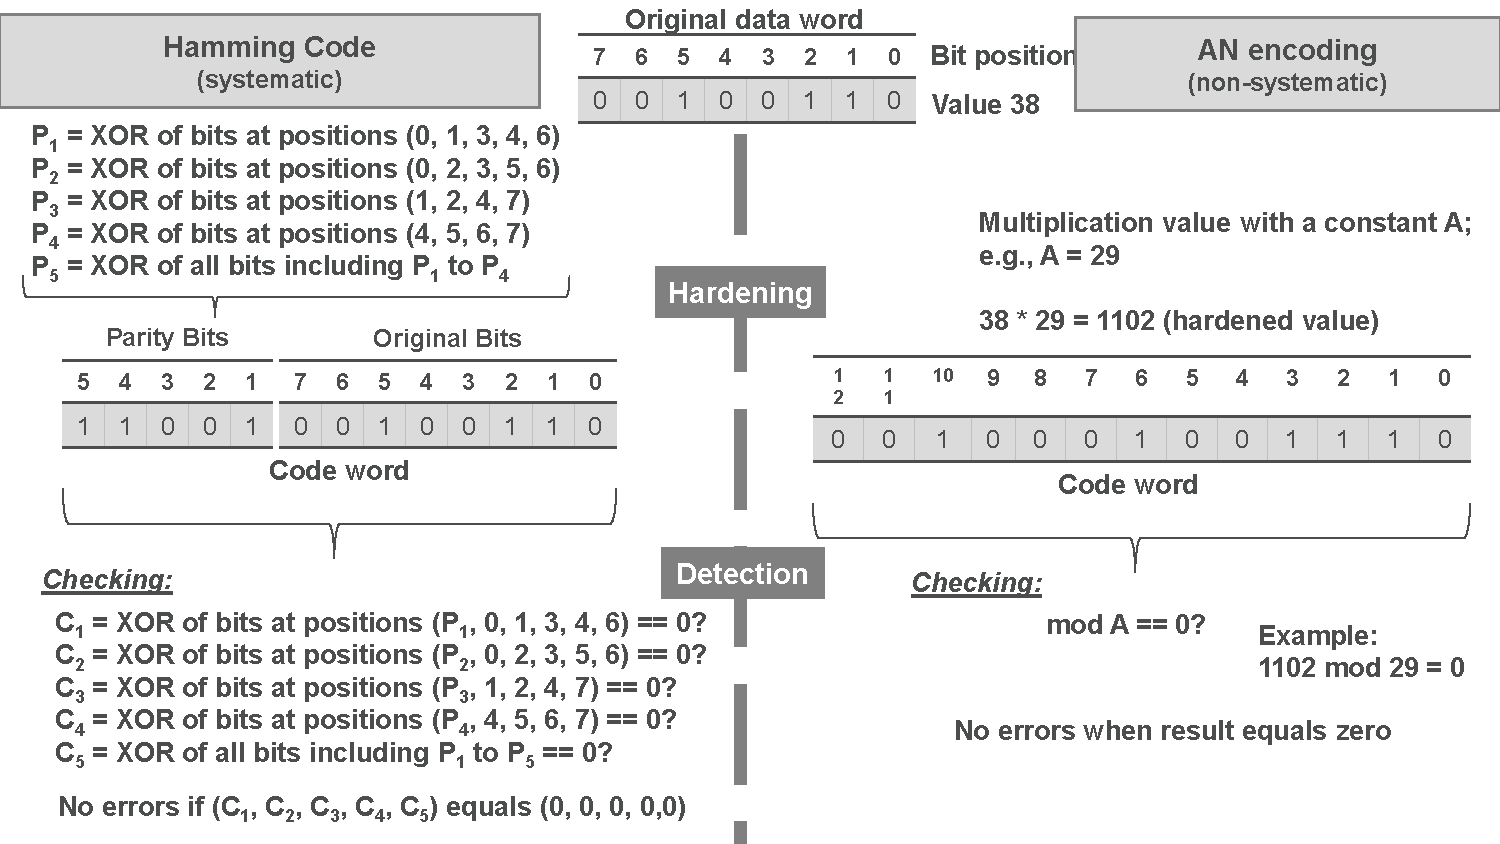
\includegraphics[width=\linewidth]{figures/hamming-an-illustration.pdf}	
	\vspace{-0.5cm}
	\caption{Illustration of Hamming and AN coding.}% using an $8$-bit value. In both cases, the hardened data words require $13$ bits and up to $2$ arbitrary bit flips are completely detectable.} 
	\label{fig:hamming-an-illustration}
	\vspace{-0.4cm}
\end{figure}


\subsection{AN Coding Justification}
\label{sec:ANCodingJustification}

As shown in Figure~\ref{fig:hamming-an-illustration}, AN coding hardens the bit representation of the original value with additional bits for error detection. This applies not only to AN coding, but also to any other error code~\cite{moon2005error}. For example, the left side of Figure~\ref{fig:hamming-an-illustration} shows the hardening using the well-known Extended Hamming code~\cite{hamming1950error}. As illustrated, the Extended Hamming Code also introduces five additional parity bits as AN coding in this setting, whereas four are computed using a bit mask (not shown here for brevity, but indicated in Figure~\ref{fig:hamming-an-illustration}) over the $8$-bit value. The fifth parity bit $P_5$ is computed over all bits. 

A difference between both codes is that AN coding is a representative of \emph{non-systematic error codes}, whereas Hamming is a \emph{systematic error code}. Systematic codes allow a separation of the original bits and additional bits. This means that the original data word is embedded as-is in the hardened representation (cf. Figure~\ref{fig:hamming-an-illustration}). In contrast, in non-systematic codes, the hardened representation does not contain the original data, so that it is not separable from the additional bits. While this makes accessing the original data faster, AN codes have a big advantage: the hardened codewords can be processed directly and each arithmetic operation also computes the additional bits, which is not the case for codes like Hamming. There, the additional bits have to be recomputed in addition to each arithmetic, introducing even more computational overhead. By that, for the database domain, codes like AN codes are preferable. Furthermore, the complete and direct processing of the hardened codewords as possible for AN codes allows the recognition of (i) errors that modify data stored in memory, (ii) errors induced during transferring on interconnects, and (iii) errors induced during computations (satisfying requirement \textbf{R1}). 

In our example (Figure~\ref{fig:hamming-an-illustration}), the specific AN code with $A=29$ and the Extended Hamming code introduce five additional bits. Both codes detect all $1$- and $2$-bit flips per code word, but in contrast to AN codes, Extended Hamming can also \emph{correct} $1$-bit errors. However, the correction property has a negative impact on the error detection capability for bit flips weights $\geq 2$ (cf. Figure~\ref{fig:8bitSDCProbability}). The chances of \emph{detecting} higher bit flip weights are much better for AN coding than for Hamming, because the SDC probability\footnote{The computation of these SDC probabilities is a topic of its own and described in Appendix~\ref{appendix:SDCProbability}} is much lower. As depicted in Figure~\ref{fig:8bitSDCProbability}, Hamming shows a zig\=zag\=curve for higher bit flip weights due to the correction capabilities and this pattern holds for all Hamming codes. Many invalid code words resulting from odd\=numbered bit flip weights ($>2$) are mistakenly corrected to a different data word, which is not detectable. Server-grade ECC main memory uses Hamming codes and thus exhibits such behavior. This is another reason for employing AN codes for \emph{detection} and why we concentrate on detection in this paper.

\begin{figure}
	\centering
	{
		\scriptsize
		\graphicspath{{gnuplot/}}
		% GNUPLOT: LaTeX picture with Postscript
\begingroup
  \makeatletter
  \providecommand\color[2][]{%
    \GenericError{(gnuplot) \space\space\space\@spaces}{%
      Package color not loaded in conjunction with
      terminal option `colourtext'%
    }{See the gnuplot documentation for explanation.%
    }{Either use 'blacktext' in gnuplot or load the package
      color.sty in LaTeX.}%
    \renewcommand\color[2][]{}%
  }%
  \providecommand\includegraphics[2][]{%
    \GenericError{(gnuplot) \space\space\space\@spaces}{%
      Package graphicx or graphics not loaded%
    }{See the gnuplot documentation for explanation.%
    }{The gnuplot epslatex terminal needs graphicx.sty or graphics.sty.}%
    \renewcommand\includegraphics[2][]{}%
  }%
  \providecommand\rotatebox[2]{#2}%
  \@ifundefined{ifGPcolor}{%
    \newif\ifGPcolor
    \GPcolortrue
  }{}%
  \@ifundefined{ifGPblacktext}{%
    \newif\ifGPblacktext
    \GPblacktexttrue
  }{}%
  % define a \g@addto@macro without @ in the name:
  \let\gplgaddtomacro\g@addto@macro
  % define empty templates for all commands taking text:
  \gdef\gplbacktext{}%
  \gdef\gplfronttext{}%
  \makeatother
  \ifGPblacktext
    % no textcolor at all
    \def\colorrgb#1{}%
    \def\colorgray#1{}%
  \else
    % gray or color?
    \ifGPcolor
      \def\colorrgb#1{\color[rgb]{#1}}%
      \def\colorgray#1{\color[gray]{#1}}%
      \expandafter\def\csname LTw\endcsname{\color{white}}%
      \expandafter\def\csname LTb\endcsname{\color{black}}%
      \expandafter\def\csname LTa\endcsname{\color{black}}%
      \expandafter\def\csname LT0\endcsname{\color[rgb]{1,0,0}}%
      \expandafter\def\csname LT1\endcsname{\color[rgb]{0,1,0}}%
      \expandafter\def\csname LT2\endcsname{\color[rgb]{0,0,1}}%
      \expandafter\def\csname LT3\endcsname{\color[rgb]{1,0,1}}%
      \expandafter\def\csname LT4\endcsname{\color[rgb]{0,1,1}}%
      \expandafter\def\csname LT5\endcsname{\color[rgb]{1,1,0}}%
      \expandafter\def\csname LT6\endcsname{\color[rgb]{0,0,0}}%
      \expandafter\def\csname LT7\endcsname{\color[rgb]{1,0.3,0}}%
      \expandafter\def\csname LT8\endcsname{\color[rgb]{0.5,0.5,0.5}}%
    \else
      % gray
      \def\colorrgb#1{\color{black}}%
      \def\colorgray#1{\color[gray]{#1}}%
      \expandafter\def\csname LTw\endcsname{\color{white}}%
      \expandafter\def\csname LTb\endcsname{\color{black}}%
      \expandafter\def\csname LTa\endcsname{\color{black}}%
      \expandafter\def\csname LT0\endcsname{\color{black}}%
      \expandafter\def\csname LT1\endcsname{\color{black}}%
      \expandafter\def\csname LT2\endcsname{\color{black}}%
      \expandafter\def\csname LT3\endcsname{\color{black}}%
      \expandafter\def\csname LT4\endcsname{\color{black}}%
      \expandafter\def\csname LT5\endcsname{\color{black}}%
      \expandafter\def\csname LT6\endcsname{\color{black}}%
      \expandafter\def\csname LT7\endcsname{\color{black}}%
      \expandafter\def\csname LT8\endcsname{\color{black}}%
    \fi
  \fi
    \setlength{\unitlength}{0.0500bp}%
    \ifx\gptboxheight\undefined%
      \newlength{\gptboxheight}%
      \newlength{\gptboxwidth}%
      \newsavebox{\gptboxtext}%
    \fi%
    \setlength{\fboxrule}{0.5pt}%
    \setlength{\fboxsep}{1pt}%
\begin{picture}(4600.00,1720.00)%
    \gplgaddtomacro\gplbacktext{%
      \csname LTb\endcsname%
      \put(604,563){\makebox(0,0)[r]{\strut{}\tiny{\num{0.01}}}}%
      \csname LTb\endcsname%
      \put(604,955){\makebox(0,0)[r]{\strut{}\tiny{\num{0.1}}}}%
      \csname LTb\endcsname%
      \put(604,1347){\makebox(0,0)[r]{\strut{}\tiny{\num{1}}}}%
      \csname LTb\endcsname%
      \put(909,272){\makebox(0,0){\strut{}$1$}}%
      \csname LTb\endcsname%
      \put(1100,272){\makebox(0,0){\strut{}$2$}}%
      \csname LTb\endcsname%
      \put(1292,272){\makebox(0,0){\strut{}$3$}}%
      \csname LTb\endcsname%
      \put(1483,272){\makebox(0,0){\strut{}$4$}}%
      \csname LTb\endcsname%
      \put(1675,272){\makebox(0,0){\strut{}$5$}}%
      \csname LTb\endcsname%
      \put(1866,272){\makebox(0,0){\strut{}$6$}}%
      \csname LTb\endcsname%
      \put(2058,272){\makebox(0,0){\strut{}$7$}}%
      \csname LTb\endcsname%
      \put(2249,272){\makebox(0,0){\strut{}$8$}}%
      \csname LTb\endcsname%
      \put(2441,272){\makebox(0,0){\strut{}$9$}}%
      \csname LTb\endcsname%
      \put(2632,272){\makebox(0,0){\strut{}$10$}}%
      \csname LTb\endcsname%
      \put(2824,272){\makebox(0,0){\strut{}$11$}}%
      \csname LTb\endcsname%
      \put(3015,272){\makebox(0,0){\strut{}$12$}}%
      \csname LTb\endcsname%
      \put(3207,272){\makebox(0,0){\strut{}$13$}}%
    }%
    \gplgaddtomacro\gplfronttext{%
      \csname LTb\endcsname%
      \put(94,896){\rotatebox{-270}{\makebox(0,0){\strut{}SDC probability}}}%
      \csname LTb\endcsname%
      \put(2057,86){\makebox(0,0){\strut{}Bit Flip Weight [\# Flipped Bits]}}%
      \csname LTb\endcsname%
      \put(2057,1533){\makebox(0,0){8-bit data, 13-bit code words}}%
      \csname LTb\endcsname%
      \put(4102,1020){\makebox(0,0)[r]{\strut{}Hamming}}%
      \csname LTb\endcsname%
      \put(4102,772){\makebox(0,0)[r]{\strut{}AN (A=29)}}%
    }%
    \gplbacktext
    \put(0,0){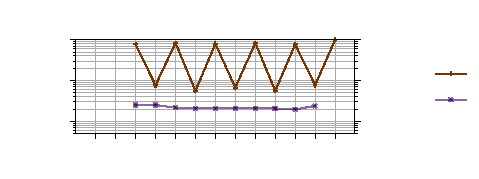
\includegraphics{hamming-single-8}}%
    \gplfronttext
  \end{picture}%
\endgroup

	}
	\vspace{-0.4cm}
	\caption{Comparison of SDC probabilities (lower is better) for Hamming and AN coding for our 8-bit data width example and $A=29$. SDC probabilities for bit flip weights $1$ and $2$ are zero, because both codes always detect these.}
	\label{fig:8bitSDCProbability}
	\vspace{-0.4cm}
\end{figure}

The very good detection capability combined with the easy adaptability of AN coding allows the satisfaction of the requirements \textbf{R2} and \textbf{R3}. The easy adaptability of AN coding means: to detect all $3$ bit flip weights or more, we only have to harden the values with a greater \(A\). This aspect is discussed in the following section in detail. Consequently, AN coding as \emph{error detection-only code} is a very good choice for bit flip detection in database systems allowing to balance detection capability and necessary overhead at run-time. A comparative performance evaluation is done in Section~\ref{sec:MicroBenchmarks}.

%\clearpage
% !TeX encoding = UTF-8
% !TeX root = sigmod2018.tex
% !TeX spellcheck = en_US
\section{Hardened Data Storage}
\label{sec:DataHardening}

In this paper, we mainly focus on \textbf{detecting bit flips} in state-of-the-art in-memory columns by tightly integrating AN coding for data hardening. Generally, the physical data storage model of column stores significantly deviates from classical row stores~\cite{DBLP:conf/sigmod/DiaconuFILMSVZ13,DBLP:journals/debu/IdreosGNMMK12,DBLP:journals/debu/LahiriNF13,DBLP:conf/vldb/StonebrakerABCCFLLMOORTZ05,DBLP:conf/icde/ZukowskiWB12}. Here, relational data is maintained using the decomposition storage model (DSM)~\cite{DBLP:conf/sigmod/CopelandK85}, where each column of a table is separately stored as a fixed-width dense array~\cite{DBLP:journals/ftdb/AbadiBHIM13}. To be able to reconstruct the tuples of a table, each column record is stored in the same (array) position across all columns of a table~\cite{DBLP:journals/ftdb/AbadiBHIM13}. Column stores typically support a fixed set of basic data types, including integers, decimal (fixed\=, or floating\=point) numbers, and strings. For fixed-width data types (e.g., integer, decimal and floating\=point), column stores utilize basic arrays of the respective type for the values of a column~\cite{DBLP:journals/ftdb/AbadiBHIM13,DBLP:journals/debu/IdreosGNMMK12}. For variable-width data types (e.g., strings), some kind of dictionary encoding is applied to transform them into fixed-width columns~\cite{DBLP:conf/sigmod/AbadiMF06,DBLP:journals/ftdb/AbadiBHIM13,DBLP:conf/sigmod/BinnigHF09}. The simplest form constructs a dictionary for an entire column sorted on frequency, and represents values as integer positions in this dictionary~\cite{DBLP:journals/ftdb/AbadiBHIM13}.


\subsection{AHEAD Columnar Storage Concept}
\label{sec:StorageConcept}

Based on this, we can ascertain that column stores consist of two main data structures: (i) \emph{data arrays} with fixed-width data types (e.g. integer and decimal numbers) and (ii) \emph{dictionaries} for variable-width data types. Thus, each base table column is stored either by means of a single data array or by a combination of a dictionary and a data array containing fixed-width integer references to the dictionary. The decision is made based on the data type of the column. Thus, our hardened storage has to protect both structures.

%Our \emph{AHEAD} approach uses byte\=aligned integer sizes for this purpose at the moment. Further details regarding the interplay of compression and AN coding are an entire subject on its own and intentionally not part of this paper.}
%Since AN code words are integers, compression techniques operating on integer data, like Null Suppression~\cite{} or Run Length Encoding~\cite{}, work well together with AN coding. 

\textbf{Hardening Data Arrays:}
For data arrays with integer or decimal values, we only have to harden values and this is done using AN coding. Regarding \textit{integer data}, this requires only multiplication with a constant factor of \(A\). These integer values are usually compressed in column stores to reduce storage and to speedup query performance~\cite{DBLP:conf/sigmod/AbadiMF06,DBLP:journals/ftdb/AbadiBHIM13,Feng:2015:BPE:2723372.2747642,Li:2013:BFS:2463676.2465322,DBLP:conf/icde/ZukowskiWB12,DBLP:conf/icde/ZukowskiHNB06}. We address that aspect using byte\=aligned integer sizes; columns are compressed in a fixed byte-oriented way. For \textit{decimal numbers}, the case is a bit more complex: for the sake of correctness and accuracy, database systems typically use fixed-point numbers and arithmetic instead of native floating point numbers (float / double)\footnote{We would like to point to the article by Thomas Neumann providing a discussion and background information on this issue~\cite{blogfloatingpoint}. In essence, rounding and precision loss problems of native floating-point numbers and operations are usually unacceptable for database systems. This is why these systems employ fixed-point arithmetic and there exist several libraries providing a variety of mathematical operators~\cite{gmp,mpir,mapm}.}. One possibility of representing fixed-point numbers is to split a number into powers of $100$, so-called \emph{limbs}, e.g. \(1,024 = 10 * 100^1 + 24 * 100^0\). In this case, each limb fits into a single byte and the position of the decimal point is stored separately, for instance in column meta data. In general, the limbs can, of course, be larger. Using this representation, there are two options for hardening a fixed\=point number: \begin{inparaenum} \item harden each limb, or \item harden the number as a whole. \end{inparaenum} The former approach requires adapting the algorithms to work on larger limbs, as each limb becomes a code word on its own. Using the latter approach allows to leave the algorithms unchanged, but unfortunately, deriving the detection capabilities for large arbitrary data widths is very expensive\footnote{See Appendix~\ref{appendix:SDCProbability} for details.}. Consequently, only the former approach is feasible.

\textbf{Hardening Dictionaries:}
Dictionaries are usually realized using index structures to efficiently encode and decode~\cite{DBLP:conf/sigmod/BinnigHF09}. In contrast to data arrays, not only data values must be hardened, but also necessary pointers within the index structures. To tackle that issue, we proposed various techniques to harden B-Trees~\cite{DBLP:conf/damon/KolditzKSHL14}. As we have shown, hardening pointer-intensive structures pose their own challenges and we refer to this solution for hardening dictionaries. Moreover, for dictionaries of integer data, AN hardening can be applied on the dictionary entries. The corresponding column contains fixed-width, AN hardened integer references to the dictionary.

\textbf{UDI-Operations:}
Our hardening approach is orthogonal to UDI-operations (Update, Delete and Insert) and does not affect them. New and modified data is usually appended at the end of a column, and hardening such data is trivial -- hardened data simply has to be inserted.


\subsection{AHEAD Adaptability}
\label{sec:Adapting}

AN coding has only one parameter \(A\) having an impact on the error detection rate as well as the necessary storage overhead. Generally, there are arbitrarily many \(A\)s to choose from and we now clarify which one to actually use. As it turns out, each \(A\) has different error detection properties with regard to the data width. This is why \(\mathbb{C}_{\mathbb{D}_\Theta}^A\) depends on both \(A\) and \(\mathbb{D}_\Theta\). It follows that for \emph{any} distinct data width, which the database supports, the error detection capabilities for a large set of \(A\)s must be computed. To compute the detection properties of an \(A\), we have to determine the Hamming distance \(d_H\) of all pairs of code words, i.e., the difference in the number of bits of any two code words. In other words, this corresponds to a bit population count of all error patterns, which leads from any valid code word to any other valid one. In the coding domain this is known as a code's \emph{distance distribution}. Next, a histogram over that distribution must be built and from that we derive the \emph{minimum Hamming distance} \(d_{H,\text{min}}\). This is the smallest Hamming distance \(\neq0\) in the distance distribution and any code is guaranteed to detect \emph{at least} all error patterns with up to \(d_{H,\text{min}}-1\) flipped bits.

\begin{table}[t!]
	\caption{Super \(A\)s for detecting a guaranteed minimum bit flip weight (min bfw), excerpt from \(|D|\in\{1,\dots,32\}\). Numbers are: \(A\)/\(|A|\)/\(|\mathbb{C}_{\mathbb{D}_\Theta}^A|\). \({}^*\)=derived by approximation, \textbf{bold}=prime, tbc=to be computed.}
	\label{tab:optimalAs}
	\vspace{-2mm}
	\centering
	\small
	\begin{tabular}{@{}c@{}rrrr@{}}
		\toprule
		\multirow{2}{*}[0.3mm]{\begin{minipage}{0.5cm}min bfw\end{minipage}} & \multicolumn{4}{c}{$|\mathbb{D}_\Theta|$} \\
		& \multicolumn{1}{c}{\(8\)}  & \multicolumn{1}{c}{\(16\)} & \multicolumn{1}{c}{\(24\)} & \multicolumn{1}{c}{\(32\)} \\
		%& \(A\) & \(|A|\) & \(|\mathbb{C}|\) & \(A\) & \(|A|\) & \(|\mathbb{C}|\) & \(A\) & \(|A|\) & \(|\mathbb{C}|\) & \(A\) & \(|A|\) & \(|\mathbb{C}|\) \\
		\midrule
		1 & \textbf{3}/2/10       & \textbf{3}/2/18   & \textbf{3}/2/26  & \textbf{3}/2/34    \\
		2 & \textbf{29}/5/13      & \textbf{61}/6/22  & \textbf{61}/6/30 & 125/7/39           \\
		3 & \textbf{233}/8/16     & \textbf{463}/9/27 & 981/10/34        & \textbf{881}/10/42 \\
		4 & 1,939/11/19           & 7,785/13/29       & 15,993/14/38     & \(16,041^*\)/14/46 \\
		5 & \textbf{13,963}/14/22 & 63,877/16/32      & tbc              & tbc                \\
		6 & 55,831/16/24          & tbc               & tbc              & tbc                \\
		\bottomrule
	\end{tabular}
	\vspace{-0.4cm}
\end{table}


As described in Appendix~\ref{appendix:SDCProbability}, obtaining the distance distribution requires a brute force approach. For each combination of bit widths \(|\mathbb{D}_\Theta|\)\footnote{We use the following notation of \(||\) for bit widths in this paper.} and \(|A|\), there exists at least one ``super \(A\)'' having optimal error detection capabilities among all other \(A\)s for that combination. For that, our optimality criterion is that that a ``super \(A\)'' has \begin{inparaenum}[(1)] \item highest \(d_{H,\text{min}}\), \item lowest bit width \(|A|\), and  \item lowest first non\=zero histogram value in its category, i.e., depending on the minimum bit flip weight (\texttt{min bfw}) and \(|\mathbb{D}_\Theta|\)\end{inparaenum}. Table~\ref{tab:optimalAs} lists an extract of ``super \(A\)s'' for different numbers of minimum bit flip weights and different data widths \(|\mathbb{D}_\Theta|\in\{8,16,24,32\}\). This table also confirms our example from Section~\ref{sec:ErrorCoding} where we used \(A\)=29 for $8$-bit data and a minimum bit flip weight of two. As depicted, we require five additional bits for the hardening. If we want to increase the minimum bit flip weight to $3$, we only have to use \(A=233\) resulting in a code word width of $16$.  In this case, the data overhead increases from $62.5\%$ (13 bit code word width) to $100\%$ (16 bit code word width for 8 bit data). Table~\ref{tab:optimalAsComplete} in the appendix lists all super \(A\)s which we obtained until now, for all \(1\leq|\mathbb{D}|\leq32\) and \(1\leq|A|\leq16\). The determination of the ``super \(A\)s'' is extremely compute-intensive, because only a brute force approach is possible. Some values are currently only approximated\footnote{The remaining correct values are still determined and will be made public on our GitHub project page \url{https://brics-db.github.io/} (see Appendix \ref{sec:GitHub})}, which is only an intermediate solution. Computations for \(1\leq|\mathbb{D}|\leq32\) and \(1\leq|A|\leq16\) took 2700 GPU hours in total on an nVidia Tesla K80 GPU cluster, including the approximations. Time complexity is in \(\mathcal{O}(2^{2\cdot|\mathbb{D}|})\) and doubles with every additional code bit. Our approximation is configurable through parameter \(M\) and reduces runtimes by \(\nicefrac{2^{|\mathbb{D}|}}{M}\) and we used \(M=1001\). For instance, runtimes are reduced by more than 5 orders of magnitude for \(|\mathbb{D}|=27\). The maximal relative error is below 1\% for code lengths which we could verify exhaustively.

To summarize, we have calculated the ``super \(A\)s'' not only for byte-aligned data widths, but also for any data widths between $1$ and $32$. The ``super \(A\)s'' adhere to our optimality criterion and are the smallest ones for detecting all bit flips up to a minimum bit flip weight. As we can see in Table~\ref{tab:optimalAs}: (1) equal or different \(A\)s are optimal for the same minimum bit flip weight and varying \(|\mathbb{D}_\Theta|\); (2) for increasing \(|\mathbb{D}_\Theta|\), we typically need larger \(|A|\)s to achieve the same detection capability; and (3) not all super \(A\)s are prime numbers. Now, we are able to use this information for a balanced data hardening with regard to a specific hardware error model (bit flip weights and rates) and data width. Additionally, data can be re-hardened at run\=time with different \(A\)s. Thus, the requirements \textbf{R2} and \textbf{R3} are adequately addressed from the storage perspective.




%we have computed the error detection capabilities of all \(A\)s for \emph{any} data width and this computation has to be done \emph{only once}. Then, we can use this information for a balanced data hardening with regard to a specific hardware error model (bit flip weights and rates) and data width. Furthermore, data can be re-hardened at run\=time with different \(A\)s. Thus, the requirements \textbf{R2} and \textbf{R3} are adequately addressed from the storage perspective.





\subsection{AHEAD Performance Improvements}
\label{sec:ANCodingImprovements}

Our third requirement \textbf{R3} is that the approach introduces as little overhead as necessary. Up to now, we have shown that the memory overhead can be adjusted according to the data width and the required error detection capabilities. Unfortunately, error detection and softening/decoding are based on division and modulo computations, which are expensive even on modern server-grade processors (cf. Section~\ref{sec:MicroBenchmarks}). We now show how to circumvent both operations. %To the best of our knowledge, the following has not yet been proposed for AN encoding. 

\textbf{Faster Softening:}
Processors' arithmetic logic units (ALUs) implicitly do computations in a residue class ring (RCR) modulo the power of two to the native register width (e.g. 8, 16, 32, 64 bits). In such an RCR, the division by any odd \(A\) can be replaced by multiplication with the \emph{multiplicative inverse} \(A^{-1}\). This cannot be done automatically by the compiler since the \(A\) will only be known at run-time and the code width may differ from the native register widths. Now, decoding becomes:
\begin{equation}
c / A \equiv c \cdot A^{-1} \equiv (d \cdot A) \cdot A^{-1} \equiv d \quad \text{mod }2^{|\mathbb{C}_{\mathbb{D}_\Theta}^A|}.
\label{eq:newdecode}
\end{equation}
The inverse can be computed with the Extended Euclidean algorithm for the RCR modulo \(2^{|\mathbb{C}_{\mathbb{D}_\Theta}^A|}\). When working with code word widths different from the processor's native register widths, the result must be masked, i.e. AND-ed with a bit mask having the appropriate \(|\mathbb{C}_{\mathbb{D}_\Theta}^A|\) least significant bits set to one. This is because there may be ones in the remaining most significant bits from the multiplication. Using the inverse has several advantages:
\begin{compactenum}
	\item Only odd numbers are coprime to any \(2^n~(n\in\mathbb{N})\) and thus have a multiplicative inverse. Consequently, it is required to use \emph{only odd} \(A\)s.
	\item Using the inverse relieves \Cref{eq:ANMulOK} from the division.
	\item The inverse enables more efficient reencoding from one code word \(c_1 = d \cdot A_1\) into another \(c_2 = d \cdot A_2\), by multiplying with the factor \(A^* = A_1^{-1} \cdot A_2\):
\end{compactenum}
\begin{gather}
c_1 \cdot A^* = (d \cdot A_1) \cdot (A_1^{-1} \cdot A_2) = d \cdot A_2 = c_2
\label{eq:newreencode}
\end{gather}
The product (\(A_1^{-1} \cdot A_2\)) is a constant factor and needs to be calculated only once, especially when reencoding multiple values.

\textbf{Faster Error Detection:}
Using the multiplicative inverse allows to get rid of the modulo operator for error detection, too. For that, as in~\cite{DBLP:conf/hase/HoffmannUDSLS14}, we must know the largest and smallest encodable data word:
\begin{align*}
d_\text{max} = \text{max}(\mathbb{D}_\Theta), \\
d_\text{min} = \text{min}(\mathbb{D}_\Theta),
\end{align*}
where the latter is required for signed integers, only. Since computations on code words must be done on register widths \(\geq|\mathbb{C}_{\mathbb{D}_\Theta}^A|\), it follows that:
\begin{equation}
|c \cdot A^{-1}| = |d^{*}| = |c| > |d| \quad \text{, }d^{*}=d.
\label{eq:decodewidth}
\end{equation}
I.e., when decoding, the resulting data word \(d^{*}\) is computed in the larger RCR (modulo \(2^{|\mathbb{C}_{\mathbb{D}_\Theta}^A|}\)) than the original data \(d\) requires (modulo \(2^{|\mathbb{D}_\Theta|}\)). This becomes very useful, because we discovered that in this case it holds that:
\begin{align}
d^* > d_\text{max} \rightarrow d^* = (d \oplus b) \label{eq:newvalidate:max} \\
d^* < d_\text{min} \rightarrow d^* = (d \oplus b) \label{eq:newvalidate:min}
\end{align}
where \(b\) is an arbitrary, \emph{detectable} bit flip of any weight and \(d^*\) was decoded from a corrupted code word. This goes further than in~\cite{DBLP:conf/hase/HoffmannUDSLS14}, because we found that it holds for \emph{any} detectable error. For signed integers, the binary representation contains ones in the \(|A|\) most significant bits (MSBs) where there should be zeros after the multiplication with the inverse. Likewise, the same holds for negative integers, but now there are \emph{zeros} in the \(|A|\) MSBs, where there should only be ones. For unsigned integers, the first test suffices, while for signed integers both tests must be conducted. Consider the following example for signed integers (sint) with \(|\mathbb{D}_\text{sint}|=|A|=8\Rightarrow|\mathbb{C}_{\mathbb{D}_\text{sint}}^A|=16\), \(d=5\), \(A=233\), and \(A^{-1}=55,129\) (unsigned) \(=-10,407\) (signed):

\vspace{-4mm}
{
	\smaller
	\begin{align}
	\begin{array}{rrlll}
	1) & 5 \cdot A = 1,165 &= \overbrace{\dots0000}^{\text{overflow}} & \overbrace{0000~0100}^{|A|} & \overbrace{1000~1101_2}^{|\mathbb{D}_\text{sint}|} \nonumber \\
	2) & 1,165 \cdot A^{-1} &= \dots0100 & 0000~0000 & 0000~0101_2 \nonumber \\
	3) & +1\text{: }1,166 \cdot A^{-1} &= \dots0100 & 1101~0111 & 0101~1110_2 \\
	4) & -1\text{: }1,164 \cdot A^{-1} &= \dots0011 & 0010~1000 & 1010~1100_2
	\end{array}
	\end{align}
}
The first line shows the encoding, with the result in binary representation. The second line is the decoding of the valid code word, with no zeros in the \(|A|\) MSBs. Lines 3 and 4 show decoding of altered code words, where \(1,165+1\) and \(1,165-1\) represent a double and single bit flip in the LSB(s), respectively. The overflow column shows that computing with non\=register widths requires masking for decoding. For the signed case, line 3 triggers the test from \Cref{eq:newvalidate:min} and line 4 the one from \Cref{eq:newvalidate:max}. Although we cannot prove this in general\footnote{A proof is very difficult due to the convolution of the multiplication.}, we could confirm this for all odd \(A\)s with \(2\leq|A|\leq16\), signed integers with \(1\leq|\mathbb{D}_\text{sint}|\leq24\), and \(|\mathbb{C}_{\mathbb{D}_\text{sint}}^A|=|A|+|\mathbb{D}_\text{sint}|\). We validated \Cref{eq:newvalidate:max,eq:newvalidate:min} using an exhaustive test over all possible code words\footnote{On a 64-core AMD Opteron 6274 server it took almost 50K CPU hours in total.}. From \Cref{eq:newvalidate:max,eq:newvalidate:min} it follows that testing an AN\=encoded data word for errors is achieved by \emph{first decoding} it and \emph{then comparing} it with the largest (and smallest) encodable data word for unsigned (signed) integers. For error testing and decoding, Hoffmann et al.~\cite{DBLP:conf/hase/HoffmannUDSLS14} use a comparable approach for their voter, but they require two comparisons and the modulo and division operators. In contrast, our approach requires one multiplication and one or two comparisons.

%\clearpage
% !TeX encoding = UTF-8
% !TeX root = vldb2018.tex
% !TeX spellcheck = en_US

\begin{figure*}%
	\captionsetup[subfigure]{justification=centering}
	\null\hfill
	\begin{subfigure}[b]{1.4cm}
		\centering
		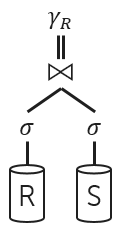
\includegraphics[scale=0.6]{figures/QP-Normal.png}
		\caption{Normal \phantom{Onetime}}
		\label{fig:QueryProcessing:normal}
	\end{subfigure}
	\hfill
	\begin{subfigure}[b]{1.5cm}
		\centering
		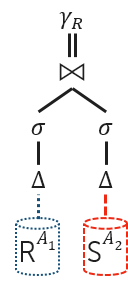
\includegraphics[scale=0.6]{figures/QP-Early.png}
		\caption{Early\\Onetime}
		\label{fig:QueryProcessing:early}
	\end{subfigure}
	\hfill
	\begin{subfigure}[b]{1.5cm}
		\centering
		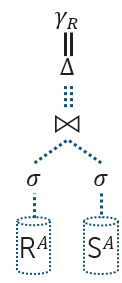
\includegraphics[scale=0.6]{figures/QP-Late1.png}
		\caption{Late\\Onetime 1}
		\label{fig:QueryProcessing:late1}
	\end{subfigure}
	\hfill
	\begin{subfigure}[b]{1.5cm}
		\centering
		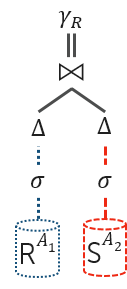
\includegraphics[scale=0.6]{figures/QP-Late2.png}
		\caption{Late\\Onetime 2}
		\label{fig:QueryProcessing:late2}
	\end{subfigure}
	\hfill
	\begin{subfigure}[b]{2cm}
		\centering
		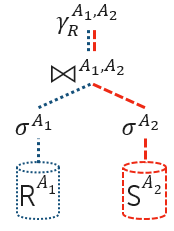
\includegraphics[scale=0.6]{figures/QP-Continuous.png}
		\caption{Continuous \phantom{Onetime}}
		\label{fig:QueryProcessing:continuous}
	\end{subfigure}
	\hfill
	\begin{subfigure}[b]{2.5cm}
		\centering
		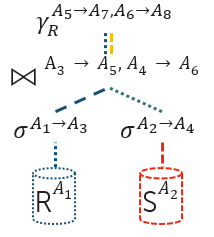
\includegraphics[scale=0.6]{figures/QP-Continuous-Reencoding.png}
		\caption{Continuous With Reencoding}
		\label{fig:QueryProcessing:reencoding}
	\end{subfigure}
	\hfill\null
	\vspace{-0.3cm}
	\caption{Illustration of the query processing variants. \(\Delta\) is a dedicated check-and-decode operator. Different \(A\)s are indicated via superscripts at the columns and operators, and via different colors and line decorations. Reencoding is indicated as \(A_1 \rightarrow A_2\).}%
	\label{fig:QueryProcessing}%
	\vspace{-0.3cm}
\end{figure*}


\section{On-the-fly Error Detection}
\label{sec:ResilientQueryProcessing}




On\=the\=fly error detection during query processing becomes now possible for both state\=of\=the\=art processing models of column\=at\=a\=time~\cite{DBLP:journals/ftdb/AbadiBHIM13,DBLP:journals/debu/IdreosGNMMK12} and vector\=at\=a\=time~\cite{DBLP:conf/icde/ZukowskiWB12} with our hardened storage concept. There are two reasons: (i) the column structure is unchanged, only the data width is increased and (ii) the values are multiplied by \(A\) and can thus be processed as before. 

\subsection{Error Detection Opportunities}

Basically, there are three opportunities for on\=the\=fly error detection as shown in \Cref{fig:QueryProcessing}, whereby \Cref{fig:QueryProcessing:normal} represents an example query execution plan (QEP) without any hardened data. In this QEP, data from two columns \(R\) and \(S\) is filtered, the results are joined, and finally grouped by column \(R\). We use this QEP, to describe our three detection possibilities during query processing. 

\textbf{Early Onetime Detection: }
As a first possibility, error detection happens only once, when touching data the very first time in the base columns (\Cref{fig:QueryProcessing:early}). For that, we introduce the \emph{detect\=and\=decode} operator \(\Delta\) taking as input a column containing hardened data and outputing a column containing the decoded data. \(\Delta\) is put before any other operator in the QEP. The physical realization of \(\Delta\) is based on a regular column scan\=operator conducting detection and decoding based on the formulas presented in Section~\ref{sec:ANCodingImprovements}. However, the disadvantage is that bit flips during the remaining query processing are not detected.

\textbf{Late Onetime Detection: }
Second, since AN coding allows arbitrary operations directly on hardened data, detection may take place in a late stage of a QEP. For instance, a hardened column can be filtered just by encoding the filter predicate with the same \(A\) the input columns are hardened with. Thus, our \emph{detect\=and\=decode} \(\Delta\) can be placed in the QEP at a point, where there are still sufficiently many tuples left for bit flip detection, e.g. before a group-by as in \Cref{fig:QueryProcessing:late1}. Operators taking multiple inputs, like joins, may encounter differently encoded inputs so that \(\Delta\) must be placed before these (\Cref{fig:QueryProcessing:late2}, \Cref{sec:AdjustmentsForContinuous} provides further details). However, the disadvantage is that bit flips are only detected at a single point and errors are propagated through the QEP. 


\textbf{Continuous Detection: }
Thus, we have to integrate bit flip detection into each and every physical operator (\Cref{fig:QueryProcessing:continuous}). This is conceptually the best solution, because bit flips are quickly detected and \(\Delta\) becomes superfluous. By that, each and every value is checked for bit flips in the columns of base tables and intermediate results.

\subsection{Adjustments for Continuous Detection}
\label{sec:AdjustmentsForContinuous}

We now focus on necessary adjustments to the query processing to realize the continuous error detection approach. 

\textbf{Error Detection Primitives for Physical Operators:}
Each physical query operator has to be adjusted to include appropriate AN coding detection primitives. We do this with a vector storing the array position of corrupted values per column. Of course, this error vector can also be affected by bit flips, so we harden it with AN coding, too. 
%In reality, an error correction activity for each detected error has to be triggered and we return to this aspect in Section~\ref{sec:Correction}. 
Further adjustments are exemplarily described for a \texttt{filter scan} operator on signed integers, as shown in \Cref{alg:continuous:filter}. For reasons of better traceability, the algorithm description is conceptually based on MonetDB primitives using their BAT data structures for columns~\cite{DBLP:journals/vldb/BonczK99}. The operator takes two inputs: (i) a single hardened input BAT and (ii) a hardened predicate (\emph{pred}\(^*\)). To provide a full\=fledged example, assume that (i) both head and tail of the input BAT are non\=virtual and encoded with different \(A\)s and (ii) the operator returns a hardened output BAT and two error vectors. First, the operator initializes the error vectors (lines 1 and 2). Variable \texttt{pos} (lines 3 and 15) is used to keep track of the position in the input BAT, so that we are able to store the error position within the input BAT. When iterating over head and tail they are first decoded (lines 5 and 6) and then tested according to \Cref{eq:newvalidate:max,eq:newvalidate:min} (lines 7 and 10). Upon detection of an error, the hardened position is stored in the appropriate error vector (lines 8 and 11). If the tail value is assumed to be valid, the filter is evaluated (line 12) and if it matches, the hardened column value is appended to the output BAT (line 13). Likewise, this pattern can be applied to all other physical operators, whereas the number of error vectors varies depending on the number of input columns.


\begin{algorithm}[t]
\caption{\texttt{Filter scan} for continuous error detection, having head and tail hardened with different \(A\)s and reencoding its output. \(^*\) denotes hardened values and BATs. Subscript \(_h\) and \(_t\) denote head and tail, respectively.}
\label{alg:continuous:filter}
\begin{algorithmic}[1]
\Require \(B_\text{in}^*\)                                     \Comment{hardened input BAT}
\Require \(A_h,A_h^{-1},A_t,A_t^{-1}\)                         \Comment{AN coding parameters}
\Require \(A_h^\prime,A_t^\prime\)                             \Comment{Reencoding parameters}
\Require \(A_\text{pos}\)                                      \Comment{Error position hardening parameter}
\Require \(d_{h,\text{max}},d_{t,\text{max}}\)                 \Comment{largest unencoded values for \(B^*_\text{in}\)}
\Require \(d_{h,\text{min}},d_{t,\text{min}}\)                 \Comment{smallest unencoded value for \(B^*_\text{in}\)}
\Require \(\circ\in\{<,\leq,=,\not=,\geq,>\}\)                 \Comment{comparison operator}
\Require \emph{pred}\(^*\)                                     \Comment{predicate encoded with \(A_t\)}
\Ensure \(B^*_\text{out}\)                                     \Comment{result BAT (same \(A\) as \(B_\text{in}^*\))}
\Ensure \(v_h, v_t\)                                           \Comment{error bit vectors for \textbf{h}ead and \textbf{t}ail}
\State \(v_h.initialize()\)                                    \Comment{allocate memory for \(v_h\)}%
                                                                   \label{lst:line:vh:init}
\State \(v_t.initialize()\)                                    \Comment{allocate memory for \(v_t\)}%
                                                                   \label{lst:line:vt:init}
\State pos \(\gets 0\)                                             \label{lst:line:pos:init}
\ForEach{(head\(^*\), tail\(^*\)) \(\in B_\text{in}^*\)}           \label{lst:line:for1}
	\State \(h \gets \text{head\(^*\)} * A_h^{-1}\)                \label{lst:line:h}
	\State \(t \gets \text{tail\(^*\)} * A_t^{-1}\)                \label{lst:line:t}
	\If{\(h < d_{h,\text{min}} \Or h > d_{h,\text{max}}\)}         \label{lst:line:if1}
		\State \(v_h.append(pos * A_\text{pos})\)                  \label{lst:line:vh:set}
	\EndIf                                                         \label{lst:line:endif1}
	\If{\(t < d_{t,\text{min}} \Or t > d_{t,\text{max}}\)}         \label{lst:line:if2}
		\State \(v_t.append(pos * A_\text{pos})\)                  \label{lst:line:vt:set}
	\ElsIf{tail\(^*\) \(\circ\) \emph{pred}\(^*\)}                 \label{lst:line:elseif2}
		\State append (\(h * A_h^\prime\), \(t * A_t^\prime\)) to \(B^*_\text{out}\)   \label{lst:line:append}
	\EndIf                                                         \label{lst:line:endif2}
	\State pos \(\gets\) pos \(+1\)                                \label{lst:line:pos:inc}
\EndFor                                                            \label{lst:line:endfor1}
\end{algorithmic}
\end{algorithm}

%Aside from this adjustment for error detection primitives, the physical operators may have to work on larger input value bit widths. However, this is a minor adjustment. 

\textbf{Physical Operations with Different \(A\)s:}
\Cref{tab:optimalAs} shows that there are different super \(A\)s for different data widths. Consequently, base columns will be hardened with different \(A\)s. In \Cref{fig:QueryProcessing} different \(A\)s are indicated by superscripts at data and operators and by different line types and colors between operators. Columns with different \(A\)s are a challenge for binary operations like joins (see \Cref{fig:QueryProcessing:continuous}). There, for different \(A\)s it holds that \((d \cdot A_1) \neq (d \cdot A_2), ~ A_1 \neq A_2\) and an equi-join would at most produce false positives, when \(d_1\cdot A_1=d_2\cdot A_2, ~ d_1 \neq d_2\). To produce correct results, binary operators have to adapt one of the inputs (hardened with \(A_1\)) to match the other's \(A_2\) by multiplying the factor \(A_1^{-1}\cdot A_2\) onto each hardened value of the first input column, or \(A_1\cdot A_2^{-1}\) onto the second. Optionally, the decoded value, which is computed for error detection and resides in a CPU register, could be multiplied by \(A_2\) only, as well. As a side effect, each operator may well harden or soften the data on-the-fly (\Cref{fig:QueryProcessing:reencoding}), called reencoding. This can, e.g., reduce the data width for intermediate results or prepare the data for the following operator (cooperative operators as introduced in~\cite{DBLP:conf/cidr/KissingerSHL13}). Consequently, it allows to adjust space requirements against reliability, i.e., multi\=bit flip detection capabilities. Reencoding is actually the same as the adaptation described for the join operator. In \Cref{fig:QueryProcessing:reencoding}, each operator reencodes its input with a new \(A\), indicated as \(A_x\rightarrow A_y\). Generally, this reencoding is a very interesting property as will be shown in the evaluation. 



\textbf{Handling of Intermediate Results:}
Because all operations can directly work on hardened data and each operator passes its hardened results to the next operator, the intermediate results are automatically hardened. There is only one special feature in column stores, namely, virtual IDs can sometimes be materialized during the query processing~\cite{DBLP:journals/ftdb/AbadiBHIM13,DBLP:journals/debu/IdreosGNMMK12}. In order to detect errors during the further processing of these virtual IDs, these IDs are automatically hardened during their generation. Differently encoded IDs can be handled as indicated above for the join.

\textbf{Bit Flip Detection in ALU Operations:}
As described in Section~\ref{sec:ErrorCoding}, AN coding allows to detect errors in certain operations of a CPU's ALU (arithmetic logic unit), which performs arithmetic, comparison and logic operations. For arithmetic operations like \(+,-,/,\dots\) (cf. \Cref{eq:ANPlusMinus,eq:ANMulUnenc,eq:ANMulOK,eq:ANDivUnenc,eq:ANDivOK}), the result can be immediately checked by multiplying with the respective \(A\)'s inverse. The checks must be anchored in the corresponding physical operators, as already described.

Error detection for comparison operations like \(<,\leq,=,\dots\) (cf. \Cref{eq:ANCompare}) is much more challenging, since comparisons are required for the detection itself. We could use a technique similar to branch-avoidance by replacing the comparison with an array access, as depicted in \Cref{fig:ANComparisonFix}. Suppose that for each comparison operator there is an infinitely large array of boolean values:
\[
	a_\text{Op}[i]\in\{\top,\bot\}, ~ \text{Op}\in\{<,\leq,\dots\}, ~ i\in\{-\infty\dots0\dots\infty\}.
\]
The difference of the two operands yields the position in the array, where we find the boolean value representing the result of the original comparison operation. For instance, \Cref{fig:ANComparisonFix:Equal} illustrates the array contents for the equality comparison. There, we compute the difference of the two operands \(c_2-c_1\) and the array contains only one \texttt{true} value at position zero, since \(c_2=c_1 \Leftrightarrow c_2-c_1=0\). Likewise, for '$<$' comparison (\Cref{fig:ANComparisonFix:Less}), we find \texttt{true} only for \(i>0\) and for '$\leq$' \texttt{true} is at all \(i\geq0\). However, infinite arrays can not be stored in memory and their contents would have to be verified at runtime as well.

\begin{figure}%
	\null\hfill
	\begin{subfigure}[t]{1in}
		\centering
		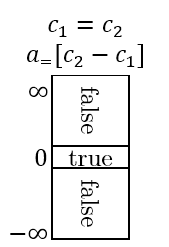
\includegraphics[width=.5in]{figures/ComparisonEquality.png}
		\caption{Equal}
		\label{fig:ANComparisonFix:Equal}
	\end{subfigure}
	\hfill
	\begin{subfigure}[t]{1in}
		\centering
		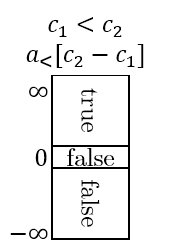
\includegraphics[width=.5in]{figures/ComparisonLessThan.png}
		\caption{Less-Than}
		\label{fig:ANComparisonFix:Less}
	\end{subfigure}
	\hfill
	\begin{subfigure}[t]{1in}
		\centering
		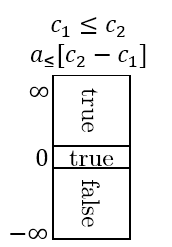
\includegraphics[width=.5in]{figures/ComparisonLessEqual.png}
		\caption{Less-or-Equal}
		\label{fig:ANComparisonFix:LessEqual}
	\end{subfigure}
	\hfill\null
	\vspace{-0.3cm}
	\caption{Replacing comparison by access to a boolean array.}%
	\label{fig:ANComparisonFix}%
	\vspace{-0.4cm}
\end{figure}


Consequently, errors in logic operations (\(\&, \|, \oplus, \neg\)) cannot be detected solely by AN coding and bit operations like AND-ing, OR-ing, XOR-ing, or inverting all bits produce \emph{invalid} code words. By that, these operations must be protected in another way. Therefore, we assume \emph{reliable} comparison and logic operations. Both areas must be considered separately in future work.

\textbf{Vectorization:}
The array-like hardened storage of columns, where only values of the very same data type are stored, allows to use vectorization (SIMD) instructions~\cite{DBLP:conf/icde/ZukowskiHNB06,willhalm2013vectorizing}. Our improved AN coding requires only multiplication and comparison, which are well supported as SIMD instructions in virtually all modern processors. Consequently, for code word widths which fit into native SIMD registers, our \emph{AHEAD} approach can be well combined with vectorizable physical operators like filter or aggregation. Willhalm et al. show how data with bit widths from 1 to 32 bits is aligned in SIMD registers to be processable, even with complex predicates and with special optimizations for each bit case~\cite{willhalm2013vectorizing}. After their alignment step, multiplication and comparison instructions for AN coding operations can be included. There are, however, some peculiarities with SIMD operations. As of now, instruction sets like Streaming SIMD Extensions (all variants until SSE4.2) and Advanced Vector Extensions 1 \& 2 do not support unsigned integer comparison, which must be emulated with 2 operations. For instance, for the unsigned ``\(>\)'' comparison in SSE4.2, instead of a single
\begin{flalign*}
& v_> = \texttt{\_mm\_cmpgt\_epu(vector(} d_0,d_1,\dots \texttt{), vector(} d_\text{max} \texttt{))}, &
\end{flalign*}
the following is required:
\begin{flalign*}
& v_\text{tmp} = \texttt{\_mm\_max\_epu(vector(} d_0,d_1,\dots \texttt{), vector(} d_\text{max} + 1 \texttt{))} & \\
& v_> = \texttt{\_mm\_cmpeq\_epi(} v_\text{tmp} \texttt{, vector(} d_0,d_1,\dots \texttt{)} &
\end{flalign*}
Afterwards, the result of the comparison can be translated into an integer using one of the \texttt{\_mm\_movemask} instruction variants. AVX-512 is supposed to provide the comparisons natively and some operations even immediately return an appropriate mask, so instead of three instructions, a single one suffices -- at least from a source code perspective.

%\subsection{Handling of Detected Bit Flips}
%\label{sec:Correction}
%
%So far, we have only been concerned with the continuous detection of bit flips during query processing. However, our \emph{AHEAD} approach also allows initial and straightforward error correction capabilities in a fine-grained way. Generally, we are currently able to detect and distinguish two kinds of errors: (i) bit flips during arithmetics and (ii) input data errors. For the latter case, however, we cannot distinguish between bit flips in main memory or those induced in interconnects. When we detect a faulty code word in the inputs, we can retransmit it, possibly several times, to correct errors induced during transmission. If we get a valid code word, processing can continue with this correct code word. If we get an invalid code word, we can assume that bits are flipped in main memory and then require an appropriate technique for error correction.
%
%Since errors during arithmetic operations are detected separately, we can also correct them separately. In principle, the operands are correct, only the arithmetic operation provides errors. To correct these errors, the single arithmetic operation can also be performed repeatedly until we get a valid resulting code word. Nevertheless, the presented error correction approaches are straightforward and should show the potential of our approach. With our \emph{AHEAD} approach, we can detect bit flips on value granularity and can find out where the error occurred. This allows us to initiate specific techniques for correction. The development of suitable techniques and the integration is subject to future work.
%




%\textbf{Ch\textsubscript{\cntincarabic{ChallengesCounter}}) Intermediate Results:}
%On the one hand, intermediate result are potentially evicted from the CPU cache to main memory. On the other hand, they may contain newly generated data, e.g. materialized OIDs from a BAT filter scan, or aggregates. A major drawback of Early Onetime Detection is, that \emph{any} bit flips in any intermediate results stay undetected. Late Onetime only mitigates this, as \(\Delta\) is further up in the query plan (cf. \Cref{fig:QueryProcessing:early,fig:QueryProcessing:late1}). In contrast, Continuous Detection does not produce unencoded intermediate results. By that, each and every value stays hardened and can be checked for bit flips. \inlinetodo{early and late do not produce hardened OIDs in intermediate results}
%
%
%
%
%
%

%
%

%
%
%
%
%\textbf{Ch\textsubscript{\cntincarabic{ChallengesCounter}}) Handling Detected Bit Flips:}
%For DRAM errors, we only set the error bits in the respective bit vectors and attempt no correction, yet. Soft errors during ALU operations do not modify the original data. The same holds for soft errors in transmissions when reading from DRAM. When it occurs during a write to DRAM, any subsequent read yields an invalid codeword and for the database it is the same as a transient error in DRAM. When a check indicates a corruption in an ALU operation or when reading from DRAM, we could try to compensate by repeating the arithmetic operation or read until a correct codeword is obtained and continue normal operation. Depending on the hardware error model, after some number of tries we would have to check whether it is a hard error. This could be tested by repeating the ALU operation on different inputs or the transmission on different memory locations. However, the hardware is typically so complex that it may be impossible to find out whether the exact same transistors are used for the repeated operations. Consequently, for now we assume that transient errors in ALU operations or transmissions for memory reads can be corrected by repeating once the operation or read. If that still yields an invalid codeword it is assumed an uncorrectable error, the error indicating bits are set in the appropriate bit vectors and affected values are skipped. Depending on the error model, a different threshold (e.g. 2 or 3 repeats) could be used, too.
%
%
%
%\cntlabel{ChallengesCounter}{ChallengesCounterTotal}
%
%AN coding allows a wide variety of integration into query processing, each with its own advantages and disadvantages. We assume that multi-bit flip rates will increase dramatically, while intermediate results, transmissions and ALU operations might be susceptible to errors, too. Only Continuous Detection provides a solution for all of the above challenges -- except C\textsubscript{1}, which is rather a requirement for the applicability of Continuous Detection. Consequently, for our \emph{AHEAD} approach, we advocate the use of \emph{continuous error detection} within main-memory database systems and particularly main-memory column stores.

%\clearpage
% !TeX encoding = UTF-8
% !TeX root = sigmod2018.tex
% !TeX spellcheck = en_US

\section{End-to-End Evaluation}
\label{sec:SSBEval}

\begin{figure*}[t!]%
	\centering
	\footnotesize
	\graphicspath{{results/ssb/report/}}
	\begin{subfigure}[t]{6.5in}
		% GNUPLOT: LaTeX picture with Postscript
\begingroup
  \makeatletter
  \providecommand\color[2][]{%
    \GenericError{(gnuplot) \space\space\space\@spaces}{%
      Package color not loaded in conjunction with
      terminal option `colourtext'%
    }{See the gnuplot documentation for explanation.%
    }{Either use 'blacktext' in gnuplot or load the package
      color.sty in LaTeX.}%
    \renewcommand\color[2][]{}%
  }%
  \providecommand\includegraphics[2][]{%
    \GenericError{(gnuplot) \space\space\space\@spaces}{%
      Package graphicx or graphics not loaded%
    }{See the gnuplot documentation for explanation.%
    }{The gnuplot epslatex terminal needs graphicx.sty or graphics.sty.}%
    \renewcommand\includegraphics[2][]{}%
  }%
  \providecommand\rotatebox[2]{#2}%
  \@ifundefined{ifGPcolor}{%
    \newif\ifGPcolor
    \GPcolortrue
  }{}%
  \@ifundefined{ifGPblacktext}{%
    \newif\ifGPblacktext
    \GPblacktexttrue
  }{}%
  % define a \g@addto@macro without @ in the name:
  \let\gplgaddtomacro\g@addto@macro
  % define empty templates for all commands taking text:
  \gdef\gplbacktext{}%
  \gdef\gplfronttext{}%
  \makeatother
  \ifGPblacktext
    % no textcolor at all
    \def\colorrgb#1{}%
    \def\colorgray#1{}%
  \else
    % gray or color?
    \ifGPcolor
      \def\colorrgb#1{\color[rgb]{#1}}%
      \def\colorgray#1{\color[gray]{#1}}%
      \expandafter\def\csname LTw\endcsname{\color{white}}%
      \expandafter\def\csname LTb\endcsname{\color{black}}%
      \expandafter\def\csname LTa\endcsname{\color{black}}%
      \expandafter\def\csname LT0\endcsname{\color[rgb]{1,0,0}}%
      \expandafter\def\csname LT1\endcsname{\color[rgb]{0,1,0}}%
      \expandafter\def\csname LT2\endcsname{\color[rgb]{0,0,1}}%
      \expandafter\def\csname LT3\endcsname{\color[rgb]{1,0,1}}%
      \expandafter\def\csname LT4\endcsname{\color[rgb]{0,1,1}}%
      \expandafter\def\csname LT5\endcsname{\color[rgb]{1,1,0}}%
      \expandafter\def\csname LT6\endcsname{\color[rgb]{0,0,0}}%
      \expandafter\def\csname LT7\endcsname{\color[rgb]{1,0.3,0}}%
      \expandafter\def\csname LT8\endcsname{\color[rgb]{0.5,0.5,0.5}}%
    \else
      % gray
      \def\colorrgb#1{\color{black}}%
      \def\colorgray#1{\color[gray]{#1}}%
      \expandafter\def\csname LTw\endcsname{\color{white}}%
      \expandafter\def\csname LTb\endcsname{\color{black}}%
      \expandafter\def\csname LTa\endcsname{\color{black}}%
      \expandafter\def\csname LT0\endcsname{\color{black}}%
      \expandafter\def\csname LT1\endcsname{\color{black}}%
      \expandafter\def\csname LT2\endcsname{\color{black}}%
      \expandafter\def\csname LT3\endcsname{\color{black}}%
      \expandafter\def\csname LT4\endcsname{\color{black}}%
      \expandafter\def\csname LT5\endcsname{\color{black}}%
      \expandafter\def\csname LT6\endcsname{\color{black}}%
      \expandafter\def\csname LT7\endcsname{\color{black}}%
      \expandafter\def\csname LT8\endcsname{\color{black}}%
    \fi
  \fi
    \setlength{\unitlength}{0.0500bp}%
    \ifx\gptboxheight\undefined%
      \newlength{\gptboxheight}%
      \newlength{\gptboxwidth}%
      \newsavebox{\gptboxtext}%
    \fi%
    \setlength{\fboxrule}{0.5pt}%
    \setlength{\fboxsep}{1pt}%
\begin{picture}(9360.00,1440.00)%
    \gplgaddtomacro\gplbacktext{%
      \csname LTb\endcsname%
      \put(412,297){\makebox(0,0)[r]{\strut{}$0$}}%
      \csname LTb\endcsname%
      \put(412,500){\makebox(0,0)[r]{\strut{}$0.5$}}%
      \csname LTb\endcsname%
      \put(412,703){\makebox(0,0)[r]{\strut{}$1$}}%
      \csname LTb\endcsname%
      \put(412,905){\makebox(0,0)[r]{\strut{}$1.5$}}%
      \csname LTb\endcsname%
      \put(412,1108){\makebox(0,0)[r]{\strut{}$2$}}%
      \csname LTb\endcsname%
      \put(412,1311){\makebox(0,0)[r]{\strut{}$2.5$}}%
      \csname LTb\endcsname%
      \put(1052,124){\makebox(0,0){\strut{}Q1.1}}%
      \csname LTb\endcsname%
      \put(1579,124){\makebox(0,0){\strut{}Q1.2}}%
      \csname LTb\endcsname%
      \put(2106,124){\makebox(0,0){\strut{}Q1.3}}%
      \csname LTb\endcsname%
      \put(2633,124){\makebox(0,0){\strut{}Q2.1}}%
      \csname LTb\endcsname%
      \put(3160,124){\makebox(0,0){\strut{}Q2.2}}%
      \csname LTb\endcsname%
      \put(3687,124){\makebox(0,0){\strut{}Q2.3}}%
      \csname LTb\endcsname%
      \put(4214,124){\makebox(0,0){\strut{}Q3.1}}%
      \csname LTb\endcsname%
      \put(4740,124){\makebox(0,0){\strut{}Q3.2}}%
      \csname LTb\endcsname%
      \put(5267,124){\makebox(0,0){\strut{}Q3.3}}%
      \csname LTb\endcsname%
      \put(5794,124){\makebox(0,0){\strut{}Q3.4}}%
      \csname LTb\endcsname%
      \put(6321,124){\makebox(0,0){\strut{}Q4.1}}%
      \csname LTb\endcsname%
      \put(6848,124){\makebox(0,0){\strut{}Q4.2}}%
      \csname LTb\endcsname%
      \put(7375,124){\makebox(0,0){\strut{}Q4.3}}%
    }%
    \gplgaddtomacro\gplfronttext{%
      \csname LTb\endcsname%
      \put(94,804){\rotatebox{-270}{\makebox(0,0){\strut{}Relative Runtime}}}%
      \csname LTb\endcsname%
      \put(8990,1174){\makebox(0,0)[r]{\strut{}Unprotected}}%
      \csname LTb\endcsname%
      \put(8990,1026){\makebox(0,0)[r]{\strut{}DMR}}%
      \csname LTb\endcsname%
      \put(8990,878){\makebox(0,0)[r]{\strut{}Early}}%
      \csname LTb\endcsname%
      \put(8990,730){\makebox(0,0)[r]{\strut{}Late}}%
      \csname LTb\endcsname%
      \put(8990,582){\makebox(0,0)[r]{\strut{}Continuous}}%
      \csname LTb\endcsname%
      \put(8990,434){\makebox(0,0)[r]{\strut{}Reencoding}}%
    }%
    \gplbacktext
    \put(0,0){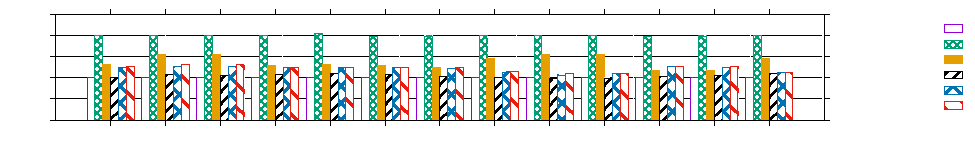
\includegraphics{norm-all_SSE}}%
    \gplfronttext
  \end{picture}%
\endgroup

	\end{subfigure}
	\vspace{-0.3cm}
	\caption{Relative SSB runtimes for vectorized (SSE4.2) execution (average over all scale factors).}%
	\label{fig:eval:runtime}%
	\vspace{-0.4cm}
\end{figure*}

We evaluate our \emph{AHEAD} approach using the analytical SSB benchmark~\cite{oneil2009ssbm}. All experiments are conducted without error induction, because the conditional SDC probabilities are known (cf. Section~\ref{sec:DataHardening}). Our system was equipped with one Intel\textsuperscript{\textregistered} Core\textsuperscript{\texttrademark} i7 6820HK CPU (\textat 2.70GHz), and 16 GB of DDR3 main memory (\textat 2133MHz) running 64\=bit Ubuntu 16.04.3 LTS using GCC 7.1.0.



\subsection{Implementation}
\label{sec:Implementation}
We implemented a self\=contained \emph{AHEAD} prototype using a column\=at\=a\=time execution model\footnote{The prototype is available on GitHub \url{https://brics-db.github.io/}, see Appendix~\ref{sec:GitHub}}, due to the following: (1) We wanted to have both protected and unprotected data to measure the appropriate runtimes in a uniform way. This requires to have operators for both available simultaneously, which would require to reimplement all physical operators in an existing DBMS. (2) We want to first show that our approach is feasible, without any side effects, so that it can then be integrated in an existing system. Our \emph{AHEAD} prototype is completely written in C++ using well-known column store concepts~\cite{DBLP:journals/ftdb/AbadiBHIM13} and supports both unprotected and hardened query processing in a unified way for comparability. For that, a separate type system allows to distinguish data types and the actual width of a type is adjusted through a mere \texttt{typedef}. Our current prototype differentiates between 8-, 16-, 32-, and 64\=bit data types, i.e. we do byte-level compression on native CPU register granularity. We call the types \texttt{tinyint}, \texttt{shortint}, \texttt{int}, and \texttt{bigint}, respectively. The hardened variants (\texttt{restiny}, \texttt{resshort}, \texttt{resint}, and \texttt{resbig}, respectively) are mapped to the next available native integer width, i.e. 16, 32, 64, and again 64 bits. For \texttt{tinyint}, this allows \(A\)s up to a width of 8\=bits, for the others \(A\)s up to 16\=bit and \texttt{bigint} is limited to 48\=bits of actual data\footnote{128-bit integer implementations like the Boost C++ library could be used to support larger integer widths, using a simple \texttt{typedef} change for scalar code.}. For strings, we use a separate data heap and the data column contains pointers to the actual string values. Our current implementation does not use dictionary compression. The physical query operators support all these data types through template programming to ease the data type specialization. Furthermore, for the vectorized operators, the template programming helps to specialize only those details of the SSE operators which require calls to specific intrinsics. For instance, the algorithm skeletons are the same for all integer types, but e.g. multiplication requires different intrinsics for 16\=bit (\texttt{\_mm\_mullo\_epi16}, \texttt{pmullw}) or 32\=bit (\texttt{\_mm\_mullo\_epi32}, \texttt{pmulld}) data, just to name two examples. We implemented both, scalar and SSE4.2 query operators, while Hash\=join and Group\=by use Google's \texttt{dense\_hash\_map}\footnote{\url{https://github.com/sparsehash}} for performance reasons. All of the $13$ SSB queries are manually written, guided by the query explanation output from MonetDB~\cite{boncz2002monet}. We chose single\=threaded execution to avoid any side\=effects and to precisely measure the overhead.


\subsection{SSB Runtime Performance}
We compare our \emph{AHEAD} approach with the \emph{Unprotected} baseline and dual modular redundancy (DMR). In the \emph{Unprotected} baseline, data is always compressed on a byte-level based on the column characteristics. \emph{DMR} uses the \emph{Unprotected} setting and replicates all data in main memory, executes each query twice sequentially, and afterwards a voter compares both results. Our \emph{AHEAD} approach hardens each column using the largest currently known \(A\) for the corresponding column data width from Table~\ref{tab:optimalAs}. Thus, compared to \emph{Unprotected} setting, \emph{AHEAD} increases the data width of each column to the next byte level. For all approaches, we measured all 13 SSB queries for scalar and vectorized (SSE4.2) execution and we varied the SSB scale factor from 1 to 10. Each single experiment ran 10 times. Figure~\ref{fig:eval:runtime} shows vectorized (SSE4.2) runtimes relative to the \emph{Unprotected} baseline. \emph{DMR} results in the expected runtime overhead of about 100\%, because each query is executed twice. For our \emph{AHEAD} detection schemes, we can draw the following conclusions:

%In total, we measured 156 query variants for all 13 SSB queries, 6 detection scheme variants (cf. Figure~\ref{fig:QueryProcessing}) and two architectures (scalar and vectorized). 

\textbf{Early Detection} has a very high initial overhead of the \(\Delta\) operator leading to an overhead between 64\% and 185\% for scalar execution (cf. Figure~\ref{fig:eval:runtime:scalar} in Appendix~\ref{sec:SSBEval:scalar}). With vectorization, early detection is much faster, because \(\Delta\) benefits so much more than the other operators, and the overhead is reduced to 18\% to 56\%.

\textbf{Late Detection} executes \(\Delta\) only on hardened data arrays prior to the aggregation or grouping and newly created intermediates like IDs are never hardened. Consequently, it checks much less values and errors are detected only very late in the query, resulting in overheads of at most 10\% for both scalar and SSE4.2 execution. Errors might add up to valid code words, so that less are detected. %in total. 
%Errors in filters cannot be detected and for both, \emph{Early} and \emph{Late}, false positives/negatives in joins and groupings cannot be detected, either.

\textbf{Continuous and Reencoding} use the same query plan as the baseline but with AN\=coding\=aware operators, where the latter reencode each operator's output. As we assume no particular error rate or bit flip weight distribution, our policy for the new \(A\) for \emph{Reencoding} is to decrease the bit width of \(A\) by $1$ for each input. For that, we use an extended version of Table~\ref{tab:optimalAs}. This is meant to simply show the feasibility of reencoding each operator output. The runtime of \emph{Continuous Detection} lies between Early and Late with about 10\% to 26\% (scalar) and 7\% to 28\% (vectorized) overhead. This is due to the tight integration of error detection in each operator. \emph{Reencoding} adds virtually no overhead to \emph{Continuous} with overheads of 10\% to 27\% (scalar) and 10\% to 31\% (SSE4.2).


\begin{figure}%
	\footnotesize
	\graphicspath{{results/ssb/}}
	% GNUPLOT: LaTeX picture with Postscript
\begingroup
  \makeatletter
  \providecommand\color[2][]{%
    \GenericError{(gnuplot) \space\space\space\@spaces}{%
      Package color not loaded in conjunction with
      terminal option `colourtext'%
    }{See the gnuplot documentation for explanation.%
    }{Either use 'blacktext' in gnuplot or load the package
      color.sty in LaTeX.}%
    \renewcommand\color[2][]{}%
  }%
  \providecommand\includegraphics[2][]{%
    \GenericError{(gnuplot) \space\space\space\@spaces}{%
      Package graphicx or graphics not loaded%
    }{See the gnuplot documentation for explanation.%
    }{The gnuplot epslatex terminal needs graphicx.sty or graphics.sty.}%
    \renewcommand\includegraphics[2][]{}%
  }%
  \providecommand\rotatebox[2]{#2}%
  \@ifundefined{ifGPcolor}{%
    \newif\ifGPcolor
    \GPcolortrue
  }{}%
  \@ifundefined{ifGPblacktext}{%
    \newif\ifGPblacktext
    \GPblacktexttrue
  }{}%
  % define a \g@addto@macro without @ in the name:
  \let\gplgaddtomacro\g@addto@macro
  % define empty templates for all commands taking text:
  \gdef\gplbacktext{}%
  \gdef\gplfronttext{}%
  \makeatother
  \ifGPblacktext
    % no textcolor at all
    \def\colorrgb#1{}%
    \def\colorgray#1{}%
  \else
    % gray or color?
    \ifGPcolor
      \def\colorrgb#1{\color[rgb]{#1}}%
      \def\colorgray#1{\color[gray]{#1}}%
      \expandafter\def\csname LTw\endcsname{\color{white}}%
      \expandafter\def\csname LTb\endcsname{\color{black}}%
      \expandafter\def\csname LTa\endcsname{\color{black}}%
      \expandafter\def\csname LT0\endcsname{\color[rgb]{1,0,0}}%
      \expandafter\def\csname LT1\endcsname{\color[rgb]{0,1,0}}%
      \expandafter\def\csname LT2\endcsname{\color[rgb]{0,0,1}}%
      \expandafter\def\csname LT3\endcsname{\color[rgb]{1,0,1}}%
      \expandafter\def\csname LT4\endcsname{\color[rgb]{0,1,1}}%
      \expandafter\def\csname LT5\endcsname{\color[rgb]{1,1,0}}%
      \expandafter\def\csname LT6\endcsname{\color[rgb]{0,0,0}}%
      \expandafter\def\csname LT7\endcsname{\color[rgb]{1,0.3,0}}%
      \expandafter\def\csname LT8\endcsname{\color[rgb]{0.5,0.5,0.5}}%
    \else
      % gray
      \def\colorrgb#1{\color{black}}%
      \def\colorgray#1{\color[gray]{#1}}%
      \expandafter\def\csname LTw\endcsname{\color{white}}%
      \expandafter\def\csname LTb\endcsname{\color{black}}%
      \expandafter\def\csname LTa\endcsname{\color{black}}%
      \expandafter\def\csname LT0\endcsname{\color{black}}%
      \expandafter\def\csname LT1\endcsname{\color{black}}%
      \expandafter\def\csname LT2\endcsname{\color{black}}%
      \expandafter\def\csname LT3\endcsname{\color{black}}%
      \expandafter\def\csname LT4\endcsname{\color{black}}%
      \expandafter\def\csname LT5\endcsname{\color{black}}%
      \expandafter\def\csname LT6\endcsname{\color{black}}%
      \expandafter\def\csname LT7\endcsname{\color{black}}%
      \expandafter\def\csname LT8\endcsname{\color{black}}%
    \fi
  \fi
    \setlength{\unitlength}{0.0500bp}%
    \ifx\gptboxheight\undefined%
      \newlength{\gptboxheight}%
      \newlength{\gptboxwidth}%
      \newsavebox{\gptboxtext}%
    \fi%
    \setlength{\fboxrule}{0.5pt}%
    \setlength{\fboxsep}{1pt}%
\begin{picture}(4160.00,1440.00)%
    \gplgaddtomacro\gplbacktext{%
      \csname LTb\endcsname%
      \put(412,421){\makebox(0,0)[r]{\strut{}$0$}}%
      \csname LTb\endcsname%
      \put(412,569){\makebox(0,0)[r]{\strut{}$0.5$}}%
      \csname LTb\endcsname%
      \put(412,718){\makebox(0,0)[r]{\strut{}$1$}}%
      \csname LTb\endcsname%
      \put(412,866){\makebox(0,0)[r]{\strut{}$1.5$}}%
      \csname LTb\endcsname%
      \put(412,1014){\makebox(0,0)[r]{\strut{}$2$}}%
      \csname LTb\endcsname%
      \put(412,1163){\makebox(0,0)[r]{\strut{}$2.5$}}%
      \csname LTb\endcsname%
      \put(412,1311){\makebox(0,0)[r]{\strut{}$3$}}%
      \csname LTb\endcsname%
      \put(1017,248){\makebox(0,0){\strut{}Unenc.}}%
      \csname LTb\endcsname%
      \put(1508,248){\makebox(0,0){\strut{}DMR}}%
      \csname LTb\endcsname%
      \put(2000,248){\makebox(0,0){\strut{}Early}}%
      \csname LTb\endcsname%
      \put(2492,248){\makebox(0,0){\strut{}Late}}%
      \csname LTb\endcsname%
      \put(2984,248){\makebox(0,0){\strut{}Cont.}}%
      \csname LTb\endcsname%
      \put(3475,248){\makebox(0,0){\strut{}Reenc.}}%
      \csname LTb\endcsname%
      \put(1263,1396){\makebox(0,0)[l]{\strut{}5.10}}%
      \csname LTb\endcsname%
      \put(1754,1396){\makebox(0,0)[l]{\strut{}5.14}}%
      \csname LTb\endcsname%
      \put(1115,1014){\rotatebox{-75}{\makebox(0,0)[l]{\strut{}2.6}}}%
      \csname LTb\endcsname%
      \put(1607,1252){\rotatebox{-70}{\makebox(0,0)[l]{\strut{}2.5}}}%
      \csname LTb\endcsname%
      \put(2098,1252){\rotatebox{-70}{\makebox(0,0)[l]{\strut{}3.5}}}%
      \csname LTb\endcsname%
      \put(2590,1074){\rotatebox{-70}{\makebox(0,0)[l]{\strut{}2.5}}}%
      \csname LTb\endcsname%
      \put(3082,1163){\rotatebox{-70}{\makebox(0,0)[l]{\strut{}2.3}}}%
      \csname LTb\endcsname%
      \put(3574,1163){\rotatebox{-70}{\makebox(0,0)[l]{\strut{}2.3}}}%
    }%
    \gplgaddtomacro\gplfronttext{%
      \csname LTb\endcsname%
      \put(94,866){\rotatebox{-270}{\makebox(0,0){\strut{}Relative Runtime}}}%
      \csname LTb\endcsname%
      \put(1813,111){\makebox(0,0)[r]{\strut{}Scalar}}%
      \csname LTb\endcsname%
      \put(2886,111){\makebox(0,0)[r]{\strut{}Vectorized}}%
    }%
    \gplbacktext
    \put(0,0){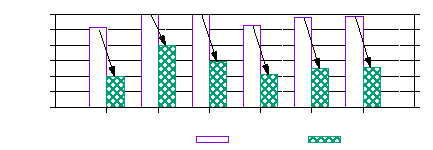
\includegraphics{vectorVSscalar1_1-1_3}}%
    \gplfronttext
  \end{picture}%
\endgroup
%
	\vspace{-1.5em}
	\caption{Scalar against vectorized runtimes (SSB 1.1 to 1.3).}%
	\label{fig:vectorVSscalar}%
	\vspace{-0.4cm}
\end{figure}


\subsection{Scalar vs. Vectorized Execution}
Having compared the detection variants per query, we now show in more detail the impact of the vectorization. We use the average over SSB queries 1.1 to 1.3 because they filter on small integer data and there the impact of vectorization is greatest. Vectorized \emph{Unprotected} serves as baseline. Figure~\ref{fig:vectorVSscalar} shows that all variants benefit greatly from SSE4.2 vectorization for queries 1.1 to 1.3. The speedup factor is shown at the arrows for each variant, as well. For \emph{Early} it is larger because \(\Delta\) benefits very much. Note that the speedups for \emph{Continous} and \emph{Reencode} are only slightly smaller than for \emph{Unprotected}, although they operate on half as many code words per SIMD instruction. Consequently, our AHEAD approach scales well using vectorization.




\begin{figure}%
	\footnotesize
	\graphicspath{{results/ssb/}}
	\null
	\begin{subfigure}{1.4in}
		% GNUPLOT: LaTeX picture with Postscript
\begingroup
  \makeatletter
  \providecommand\color[2][]{%
    \GenericError{(gnuplot) \space\space\space\@spaces}{%
      Package color not loaded in conjunction with
      terminal option `colourtext'%
    }{See the gnuplot documentation for explanation.%
    }{Either use 'blacktext' in gnuplot or load the package
      color.sty in LaTeX.}%
    \renewcommand\color[2][]{}%
  }%
  \providecommand\includegraphics[2][]{%
    \GenericError{(gnuplot) \space\space\space\@spaces}{%
      Package graphicx or graphics not loaded%
    }{See the gnuplot documentation for explanation.%
    }{The gnuplot epslatex terminal needs graphicx.sty or graphics.sty.}%
    \renewcommand\includegraphics[2][]{}%
  }%
  \providecommand\rotatebox[2]{#2}%
  \@ifundefined{ifGPcolor}{%
    \newif\ifGPcolor
    \GPcolortrue
  }{}%
  \@ifundefined{ifGPblacktext}{%
    \newif\ifGPblacktext
    \GPblacktexttrue
  }{}%
  % define a \g@addto@macro without @ in the name:
  \let\gplgaddtomacro\g@addto@macro
  % define empty templates for all commands taking text:
  \gdef\gplbacktext{}%
  \gdef\gplfronttext{}%
  \makeatother
  \ifGPblacktext
    % no textcolor at all
    \def\colorrgb#1{}%
    \def\colorgray#1{}%
  \else
    % gray or color?
    \ifGPcolor
      \def\colorrgb#1{\color[rgb]{#1}}%
      \def\colorgray#1{\color[gray]{#1}}%
      \expandafter\def\csname LTw\endcsname{\color{white}}%
      \expandafter\def\csname LTb\endcsname{\color{black}}%
      \expandafter\def\csname LTa\endcsname{\color{black}}%
      \expandafter\def\csname LT0\endcsname{\color[rgb]{1,0,0}}%
      \expandafter\def\csname LT1\endcsname{\color[rgb]{0,1,0}}%
      \expandafter\def\csname LT2\endcsname{\color[rgb]{0,0,1}}%
      \expandafter\def\csname LT3\endcsname{\color[rgb]{1,0,1}}%
      \expandafter\def\csname LT4\endcsname{\color[rgb]{0,1,1}}%
      \expandafter\def\csname LT5\endcsname{\color[rgb]{1,1,0}}%
      \expandafter\def\csname LT6\endcsname{\color[rgb]{0,0,0}}%
      \expandafter\def\csname LT7\endcsname{\color[rgb]{1,0.3,0}}%
      \expandafter\def\csname LT8\endcsname{\color[rgb]{0.5,0.5,0.5}}%
    \else
      % gray
      \def\colorrgb#1{\color{black}}%
      \def\colorgray#1{\color[gray]{#1}}%
      \expandafter\def\csname LTw\endcsname{\color{white}}%
      \expandafter\def\csname LTb\endcsname{\color{black}}%
      \expandafter\def\csname LTa\endcsname{\color{black}}%
      \expandafter\def\csname LT0\endcsname{\color{black}}%
      \expandafter\def\csname LT1\endcsname{\color{black}}%
      \expandafter\def\csname LT2\endcsname{\color{black}}%
      \expandafter\def\csname LT3\endcsname{\color{black}}%
      \expandafter\def\csname LT4\endcsname{\color{black}}%
      \expandafter\def\csname LT5\endcsname{\color{black}}%
      \expandafter\def\csname LT6\endcsname{\color{black}}%
      \expandafter\def\csname LT7\endcsname{\color{black}}%
      \expandafter\def\csname LT8\endcsname{\color{black}}%
    \fi
  \fi
    \setlength{\unitlength}{0.0500bp}%
    \ifx\gptboxheight\undefined%
      \newlength{\gptboxheight}%
      \newlength{\gptboxwidth}%
      \newsavebox{\gptboxtext}%
    \fi%
    \setlength{\fboxrule}{0.5pt}%
    \setlength{\fboxsep}{1pt}%
\begin{picture}(2000.00,1440.00)%
    \gplgaddtomacro\gplbacktext{%
      \csname LTb\endcsname%
      \put(380,421){\makebox(0,0)[r]{\strut{}$0$}}%
      \csname LTb\endcsname%
      \put(380,561){\makebox(0,0)[r]{\strut{}$0.2$}}%
      \csname LTb\endcsname%
      \put(380,701){\makebox(0,0)[r]{\strut{}$0.4$}}%
      \csname LTb\endcsname%
      \put(380,841){\makebox(0,0)[r]{\strut{}$0.6$}}%
      \csname LTb\endcsname%
      \put(380,982){\makebox(0,0)[r]{\strut{}$0.8$}}%
      \csname LTb\endcsname%
      \put(380,1122){\makebox(0,0)[r]{\strut{}$1$}}%
      \csname LTb\endcsname%
      \put(380,1262){\makebox(0,0)[r]{\strut{}$1.2$}}%
      \csname LTb\endcsname%
      \put(380,1402){\makebox(0,0)[r]{\strut{}$1.4$}}%
      \csname LTb\endcsname%
      \put(794,248){\makebox(0,0){\strut{}1}}%
      \csname LTb\endcsname%
      \put(1095,248){\makebox(0,0){\strut{}2}}%
      \csname LTb\endcsname%
      \put(1397,248){\makebox(0,0){\strut{}3}}%
      \csname LTb\endcsname%
      \put(1698,248){\makebox(0,0){\strut{}4$^*$}}%
    }%
    \gplgaddtomacro\gplfronttext{%
      \csname LTb\endcsname%
      \put(94,787){\rotatebox{-270}{\makebox(0,0){\strut{}Relative Runtime}}}%
      \csname LTb\endcsname%
      \put(941,111){\makebox(0,0)[r]{\strut{}Scalar}}%
      \csname LTb\endcsname%
      \put(1630,111){\makebox(0,0)[r]{\strut{}SSE4.2}}%
    }%
    \gplbacktext
    \put(0,0){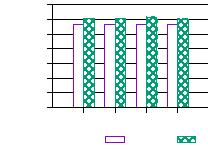
\includegraphics{minbfw_runtime}}%
    \gplfronttext
  \end{picture}%
\endgroup
%
		\vspace{-0.5em}
		\caption{Runtime}
		\label{fig:minbfw:runtime}
	\end{subfigure}
	\hfill
	\begin{subfigure}{1.7in}
		% GNUPLOT: LaTeX picture with Postscript
\begingroup
  \makeatletter
  \providecommand\color[2][]{%
    \GenericError{(gnuplot) \space\space\space\@spaces}{%
      Package color not loaded in conjunction with
      terminal option `colourtext'%
    }{See the gnuplot documentation for explanation.%
    }{Either use 'blacktext' in gnuplot or load the package
      color.sty in LaTeX.}%
    \renewcommand\color[2][]{}%
  }%
  \providecommand\includegraphics[2][]{%
    \GenericError{(gnuplot) \space\space\space\@spaces}{%
      Package graphicx or graphics not loaded%
    }{See the gnuplot documentation for explanation.%
    }{The gnuplot epslatex terminal needs graphicx.sty or graphics.sty.}%
    \renewcommand\includegraphics[2][]{}%
  }%
  \providecommand\rotatebox[2]{#2}%
  \@ifundefined{ifGPcolor}{%
    \newif\ifGPcolor
    \GPcolortrue
  }{}%
  \@ifundefined{ifGPblacktext}{%
    \newif\ifGPblacktext
    \GPblacktexttrue
  }{}%
  % define a \g@addto@macro without @ in the name:
  \let\gplgaddtomacro\g@addto@macro
  % define empty templates for all commands taking text:
  \gdef\gplbacktext{}%
  \gdef\gplfronttext{}%
  \makeatother
  \ifGPblacktext
    % no textcolor at all
    \def\colorrgb#1{}%
    \def\colorgray#1{}%
  \else
    % gray or color?
    \ifGPcolor
      \def\colorrgb#1{\color[rgb]{#1}}%
      \def\colorgray#1{\color[gray]{#1}}%
      \expandafter\def\csname LTw\endcsname{\color{white}}%
      \expandafter\def\csname LTb\endcsname{\color{black}}%
      \expandafter\def\csname LTa\endcsname{\color{black}}%
      \expandafter\def\csname LT0\endcsname{\color[rgb]{1,0,0}}%
      \expandafter\def\csname LT1\endcsname{\color[rgb]{0,1,0}}%
      \expandafter\def\csname LT2\endcsname{\color[rgb]{0,0,1}}%
      \expandafter\def\csname LT3\endcsname{\color[rgb]{1,0,1}}%
      \expandafter\def\csname LT4\endcsname{\color[rgb]{0,1,1}}%
      \expandafter\def\csname LT5\endcsname{\color[rgb]{1,1,0}}%
      \expandafter\def\csname LT6\endcsname{\color[rgb]{0,0,0}}%
      \expandafter\def\csname LT7\endcsname{\color[rgb]{1,0.3,0}}%
      \expandafter\def\csname LT8\endcsname{\color[rgb]{0.5,0.5,0.5}}%
    \else
      % gray
      \def\colorrgb#1{\color{black}}%
      \def\colorgray#1{\color[gray]{#1}}%
      \expandafter\def\csname LTw\endcsname{\color{white}}%
      \expandafter\def\csname LTb\endcsname{\color{black}}%
      \expandafter\def\csname LTa\endcsname{\color{black}}%
      \expandafter\def\csname LT0\endcsname{\color{black}}%
      \expandafter\def\csname LT1\endcsname{\color{black}}%
      \expandafter\def\csname LT2\endcsname{\color{black}}%
      \expandafter\def\csname LT3\endcsname{\color{black}}%
      \expandafter\def\csname LT4\endcsname{\color{black}}%
      \expandafter\def\csname LT5\endcsname{\color{black}}%
      \expandafter\def\csname LT6\endcsname{\color{black}}%
      \expandafter\def\csname LT7\endcsname{\color{black}}%
      \expandafter\def\csname LT8\endcsname{\color{black}}%
    \fi
  \fi
    \setlength{\unitlength}{0.0500bp}%
    \ifx\gptboxheight\undefined%
      \newlength{\gptboxheight}%
      \newlength{\gptboxwidth}%
      \newsavebox{\gptboxtext}%
    \fi%
    \setlength{\fboxrule}{0.5pt}%
    \setlength{\fboxsep}{1pt}%
\begin{picture}(2440.00,1440.00)%
    \gplgaddtomacro\gplbacktext{%
      \csname LTb\endcsname%
      \put(380,545){\makebox(0,0)[r]{\strut{}$0$}}%
      \csname LTb\endcsname%
      \put(380,716){\makebox(0,0)[r]{\strut{}$0.5$}}%
      \csname LTb\endcsname%
      \put(380,888){\makebox(0,0)[r]{\strut{}$1$}}%
      \csname LTb\endcsname%
      \put(380,1059){\makebox(0,0)[r]{\strut{}$1.5$}}%
      \csname LTb\endcsname%
      \put(380,1231){\makebox(0,0)[r]{\strut{}$2$}}%
      \csname LTb\endcsname%
      \put(380,1402){\makebox(0,0)[r]{\strut{}$2.5$}}%
      \csname LTb\endcsname%
      \put(882,372){\makebox(0,0){\strut{}1}}%
      \csname LTb\endcsname%
      \put(1271,372){\makebox(0,0){\strut{}2}}%
      \csname LTb\endcsname%
      \put(1661,372){\makebox(0,0){\strut{}3}}%
      \csname LTb\endcsname%
      \put(2050,372){\makebox(0,0){\strut{}4$^*$}}%
    }%
    \gplgaddtomacro\gplfronttext{%
      \csname LTb\endcsname%
      \put(94,725){\rotatebox{-270}{\makebox(0,0){\strut{}Relative Consumption}}}%
      \csname LTb\endcsname%
      \put(1161,235){\makebox(0,0)[r]{\strut{}Unprotected}}%
      \csname LTb\endcsname%
      \put(1161,111){\makebox(0,0)[r]{\strut{}Continuous}}%
      \csname LTb\endcsname%
      \put(2170,235){\makebox(0,0)[r]{\strut{}Bit-Packed}}%
      \csname LTb\endcsname%
      \put(1077,1128){\rotatebox{90}{\makebox(0,0)[l]{\strut{}1.43}}}%
      \csname LTb\endcsname%
      \put(1466,1128){\rotatebox{90}{\makebox(0,0)[l]{\strut{}1.49}}}%
      \csname LTb\endcsname%
      \put(1855,1128){\rotatebox{90}{\makebox(0,0)[l]{\strut{}1.55}}}%
      \csname LTb\endcsname%
      \put(2244,1128){\rotatebox{90}{\makebox(0,0)[l]{\strut{}1.61}}}%
    }%
    \gplbacktext
    \put(0,0){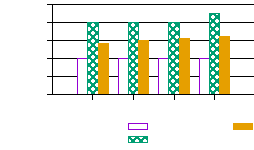
\includegraphics{minbfw_consumption}}%
    \gplfronttext
  \end{picture}%
\endgroup
%
		\vspace{-0.5em}
		\caption{Storage}
		\label{fig:minbfw:storage}
	\end{subfigure}
	\null
	\vspace{-1.5em}
	\caption{SSB query 1.1 runtime and storage comparison for \emph{Continuous} with different min bfw's (x axis). $4^*$: we increased \texttt{restiny} size to 32 bits to allow \(|A|>8\).}%
	\label{fig:minbfw}%
	\vspace{-0.5cm}
\end{figure}

%It was shown that data centers already exhibit bit flip weights (bfw's) of up to 4~\cite{}.



\subsection{Influence of Bit Flip Weight}
Up to now, we used the largest \(A\) for data hardening in our experiments. We will now investigate the influence of different \(A\)s on the runtime and storage overhead of the \emph{Continuous} variant. For each hardened data type, we vary the \(A\) of all base and intermediate columns to the smallest one for guaranteed minimum bit flip weights (\emph{min bfw}) $1$ to $4$ from Table~\ref{tab:optimalAs}. We chose this scenario, because Kim et al.~\cite{DBLP:conf/isca/KimDKFLLWLM14} observed one to four bit flips in all newer DRAM modules. For the case of $4$, we let the \texttt{restiny} datatype be 32 bits wide to allow $|A|>8$. Due to our type system, this is a simple \texttt{typedef} change. Figure~\ref{fig:minbfw:runtime} shows the runtimes as in Figure~\ref{fig:eval:runtime}, while Figure~\ref{fig:minbfw:storage} shows the storage overhead. Runtimes differ only slightly for both scalar and SSE4.2 execution. With \emph{Continuous}, the storage consumption doubles for \emph{min bfw} $1$ to $3$, because we only work on native register widths. For \emph{min bfw} $4$, the storage overhead is slightly higher (126\%), since \texttt{restiny} is twice as big. This shows the limitation of our current byte-oriented compression. Willhalm et al. showed how to store data in a bit-packed fashion and how to evaluate even complex filter predicates in a vectorized manner~\cite{Willhalm:2009:SUF:1687627.1687671,willhalm2013vectorizing}. To overcome our current implementation limitation, we could use their approach. To show the benefit, we projected the storage consumption for \emph{bit-packed} compression in Figure~\ref{fig:minbfw:storage} as well, which displays potentials for reducing the memory overhead of our \emph{AHEAD} approach. Since bit-packing reduces the load on the memory subsystem, this \emph{might} improve query runtimes, too, but that remains to be seen.

%We project the consumption when \emph{bit-packed} compression was used in Figure~\ref{fig:minbfw:storage}, which displays potentials for reducing the memory overhead of our \emph{AHEAD} approach. The teaser Figure~\ref{fig:teaser:memory} uses the projected numbers because in a real system \emph{AHEAD} would be implemented with bit-packed compression, e.g. after~\cite{Willhalm:2009:SUF:1687627.1687671,willhalm2013vectorizing}.







%\subsection{Memory Overhead}
%\begin{table}%
%{
%	\footnotesize
%	\begin{tabular}{crrrrrr}
%		\toprule
%		 & Unenc. & DMR & Early & Late & Cont. & Bit-Packed  \\
%		\midrule
%		Min & 1.00 & 2.00 & 1.25 & 1.21 & 1.91 & 1.43        \\
%		Max & 1.00 & 2.01 & 152.76 & 1.27 & 2.00 & 1.58      \\
%		Avg & 1.00 & 2.00 & 29.50 & 1.25 & 1.98 & 1.50       \\
%		Median & 1.00 & 2.00 & 3.86 & 1.25 & 1.99 & 1.50     \\
%		\bottomrule
%	\end{tabular}
%}
%\caption{Memory consumption of intermediate results (over all SSB queries and scale factors)}
%\label{tab:memoryconsumption}
%\end{table}

%\clearpage
\begin{figure*}[t!]%
	\graphicspath{{results/microbenchmarks/}}
	\scriptsize
	\null\hfill
	\begin{subfigure}[t]{0.2in}
		% GNUPLOT: LaTeX picture with Postscript
\begingroup
  \makeatletter
  \providecommand\color[2][]{%
    \GenericError{(gnuplot) \space\space\space\@spaces}{%
      Package color not loaded in conjunction with
      terminal option `colourtext'%
    }{See the gnuplot documentation for explanation.%
    }{Either use 'blacktext' in gnuplot or load the package
      color.sty in LaTeX.}%
    \renewcommand\color[2][]{}%
  }%
  \providecommand\includegraphics[2][]{%
    \GenericError{(gnuplot) \space\space\space\@spaces}{%
      Package graphicx or graphics not loaded%
    }{See the gnuplot documentation for explanation.%
    }{The gnuplot epslatex terminal needs graphicx.sty or graphics.sty.}%
    \renewcommand\includegraphics[2][]{}%
  }%
  \providecommand\rotatebox[2]{#2}%
  \@ifundefined{ifGPcolor}{%
    \newif\ifGPcolor
    \GPcolortrue
  }{}%
  \@ifundefined{ifGPblacktext}{%
    \newif\ifGPblacktext
    \GPblacktexttrue
  }{}%
  % define a \g@addto@macro without @ in the name:
  \let\gplgaddtomacro\g@addto@macro
  % define empty templates for all commands taking text:
  \gdef\gplbacktext{}%
  \gdef\gplfronttext{}%
  \makeatother
  \ifGPblacktext
    % no textcolor at all
    \def\colorrgb#1{}%
    \def\colorgray#1{}%
  \else
    % gray or color?
    \ifGPcolor
      \def\colorrgb#1{\color[rgb]{#1}}%
      \def\colorgray#1{\color[gray]{#1}}%
      \expandafter\def\csname LTw\endcsname{\color{white}}%
      \expandafter\def\csname LTb\endcsname{\color{black}}%
      \expandafter\def\csname LTa\endcsname{\color{black}}%
      \expandafter\def\csname LT0\endcsname{\color[rgb]{1,0,0}}%
      \expandafter\def\csname LT1\endcsname{\color[rgb]{0,1,0}}%
      \expandafter\def\csname LT2\endcsname{\color[rgb]{0,0,1}}%
      \expandafter\def\csname LT3\endcsname{\color[rgb]{1,0,1}}%
      \expandafter\def\csname LT4\endcsname{\color[rgb]{0,1,1}}%
      \expandafter\def\csname LT5\endcsname{\color[rgb]{1,1,0}}%
      \expandafter\def\csname LT6\endcsname{\color[rgb]{0,0,0}}%
      \expandafter\def\csname LT7\endcsname{\color[rgb]{1,0.3,0}}%
      \expandafter\def\csname LT8\endcsname{\color[rgb]{0.5,0.5,0.5}}%
    \else
      % gray
      \def\colorrgb#1{\color{black}}%
      \def\colorgray#1{\color[gray]{#1}}%
      \expandafter\def\csname LTw\endcsname{\color{white}}%
      \expandafter\def\csname LTb\endcsname{\color{black}}%
      \expandafter\def\csname LTa\endcsname{\color{black}}%
      \expandafter\def\csname LT0\endcsname{\color{black}}%
      \expandafter\def\csname LT1\endcsname{\color{black}}%
      \expandafter\def\csname LT2\endcsname{\color{black}}%
      \expandafter\def\csname LT3\endcsname{\color{black}}%
      \expandafter\def\csname LT4\endcsname{\color{black}}%
      \expandafter\def\csname LT5\endcsname{\color{black}}%
      \expandafter\def\csname LT6\endcsname{\color{black}}%
      \expandafter\def\csname LT7\endcsname{\color{black}}%
      \expandafter\def\csname LT8\endcsname{\color{black}}%
    \fi
  \fi
    \setlength{\unitlength}{0.0500bp}%
    \ifx\gptboxheight\undefined%
      \newlength{\gptboxheight}%
      \newlength{\gptboxwidth}%
      \newsavebox{\gptboxtext}%
    \fi%
    \setlength{\fboxrule}{0.5pt}%
    \setlength{\fboxsep}{1pt}%
\begin{picture}(280.00,1800.00)%
    \gplgaddtomacro\gplbacktext{%
      \csname LTb\endcsname%
      \put(167,566){\rotatebox{90}{\makebox(0,0)[l]{\strut{}Scalar Runtime [s]}}}%
    }%
    \gplgaddtomacro\gplfronttext{%
    }%
    \gplbacktext
    \put(0,0){
\includegraphics{plot_paper_ylabel_scalar}}%
    \gplfronttext
  \end{picture}%
\endgroup

	\end{subfigure}
	\hfill
	\begin{subfigure}[t]{1.3in}
		% GNUPLOT: LaTeX picture with Postscript
\begingroup
  \makeatletter
  \providecommand\color[2][]{%
    \GenericError{(gnuplot) \space\space\space\@spaces}{%
      Package color not loaded in conjunction with
      terminal option `colourtext'%
    }{See the gnuplot documentation for explanation.%
    }{Either use 'blacktext' in gnuplot or load the package
      color.sty in LaTeX.}%
    \renewcommand\color[2][]{}%
  }%
  \providecommand\includegraphics[2][]{%
    \GenericError{(gnuplot) \space\space\space\@spaces}{%
      Package graphicx or graphics not loaded%
    }{See the gnuplot documentation for explanation.%
    }{The gnuplot epslatex terminal needs graphicx.sty or graphics.sty.}%
    \renewcommand\includegraphics[2][]{}%
  }%
  \providecommand\rotatebox[2]{#2}%
  \@ifundefined{ifGPcolor}{%
    \newif\ifGPcolor
    \GPcolortrue
  }{}%
  \@ifundefined{ifGPblacktext}{%
    \newif\ifGPblacktext
    \GPblacktexttrue
  }{}%
  % define a \g@addto@macro without @ in the name:
  \let\gplgaddtomacro\g@addto@macro
  % define empty templates for all commands taking text:
  \gdef\gplbacktext{}%
  \gdef\gplfronttext{}%
  \makeatother
  \ifGPblacktext
    % no textcolor at all
    \def\colorrgb#1{}%
    \def\colorgray#1{}%
  \else
    % gray or color?
    \ifGPcolor
      \def\colorrgb#1{\color[rgb]{#1}}%
      \def\colorgray#1{\color[gray]{#1}}%
      \expandafter\def\csname LTw\endcsname{\color{white}}%
      \expandafter\def\csname LTb\endcsname{\color{black}}%
      \expandafter\def\csname LTa\endcsname{\color{black}}%
      \expandafter\def\csname LT0\endcsname{\color[rgb]{1,0,0}}%
      \expandafter\def\csname LT1\endcsname{\color[rgb]{0,1,0}}%
      \expandafter\def\csname LT2\endcsname{\color[rgb]{0,0,1}}%
      \expandafter\def\csname LT3\endcsname{\color[rgb]{1,0,1}}%
      \expandafter\def\csname LT4\endcsname{\color[rgb]{0,1,1}}%
      \expandafter\def\csname LT5\endcsname{\color[rgb]{1,1,0}}%
      \expandafter\def\csname LT6\endcsname{\color[rgb]{0,0,0}}%
      \expandafter\def\csname LT7\endcsname{\color[rgb]{1,0.3,0}}%
      \expandafter\def\csname LT8\endcsname{\color[rgb]{0.5,0.5,0.5}}%
    \else
      % gray
      \def\colorrgb#1{\color{black}}%
      \def\colorgray#1{\color[gray]{#1}}%
      \expandafter\def\csname LTw\endcsname{\color{white}}%
      \expandafter\def\csname LTb\endcsname{\color{black}}%
      \expandafter\def\csname LTa\endcsname{\color{black}}%
      \expandafter\def\csname LT0\endcsname{\color{black}}%
      \expandafter\def\csname LT1\endcsname{\color{black}}%
      \expandafter\def\csname LT2\endcsname{\color{black}}%
      \expandafter\def\csname LT3\endcsname{\color{black}}%
      \expandafter\def\csname LT4\endcsname{\color{black}}%
      \expandafter\def\csname LT5\endcsname{\color{black}}%
      \expandafter\def\csname LT6\endcsname{\color{black}}%
      \expandafter\def\csname LT7\endcsname{\color{black}}%
      \expandafter\def\csname LT8\endcsname{\color{black}}%
    \fi
  \fi
    \setlength{\unitlength}{0.0500bp}%
    \ifx\gptboxheight\undefined%
      \newlength{\gptboxheight}%
      \newlength{\gptboxwidth}%
      \newsavebox{\gptboxtext}%
    \fi%
    \setlength{\fboxrule}{0.5pt}%
    \setlength{\fboxsep}{1pt}%
\begin{picture}(1860.00,1800.00)%
    \gplgaddtomacro\gplbacktext{%
      \csname LTb\endcsname%
      \put(192,372){\makebox(0,0)[r]{\strut{}$0$}}%
      \csname LTb\endcsname%
      \put(192,502){\makebox(0,0)[r]{\strut{}$0.2$}}%
      \csname LTb\endcsname%
      \put(192,633){\makebox(0,0)[r]{\strut{}$0.4$}}%
      \csname LTb\endcsname%
      \put(192,763){\makebox(0,0)[r]{\strut{}$0.6$}}%
      \csname LTb\endcsname%
      \put(192,893){\makebox(0,0)[r]{\strut{}$0.8$}}%
      \csname LTb\endcsname%
      \put(192,1024){\makebox(0,0)[r]{\strut{}$1$}}%
      \csname LTb\endcsname%
      \put(192,1154){\makebox(0,0)[r]{\strut{}$1.2$}}%
      \csname LTb\endcsname%
      \put(192,1284){\makebox(0,0)[r]{\strut{}$1.4$}}%
      \csname LTb\endcsname%
      \put(192,1414){\makebox(0,0)[r]{\strut{}$1.6$}}%
      \csname LTb\endcsname%
      \put(192,1545){\makebox(0,0)[r]{\strut{}$1.8$}}%
      \csname LTb\endcsname%
      \put(192,1675){\makebox(0,0)[r]{\strut{}$2$}}%
      \csname LTb\endcsname%
      \put(256,248){\makebox(0,0){\strut{}$2^{0}$}}%
      \csname LTb\endcsname%
      \put(564,248){\makebox(0,0){\strut{}$2^{2}$}}%
      \csname LTb\endcsname%
      \put(872,248){\makebox(0,0){\strut{}$2^{4}$}}%
      \csname LTb\endcsname%
      \put(1179,248){\makebox(0,0){\strut{}$2^{6}$}}%
      \csname LTb\endcsname%
      \put(1487,248){\makebox(0,0){\strut{}$2^{8}$}}%
      \csname LTb\endcsname%
      \put(1795,248){\makebox(0,0){\strut{}$2^{10}$}}%
    }%
    \gplgaddtomacro\gplfronttext{%
      \csname LTb\endcsname%
      \put(1025,62){\makebox(0,0){\strut{}unroll / block size}}%
    }%
    \gplbacktext
    \put(0,0){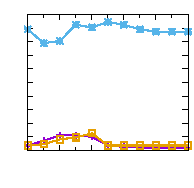
\includegraphics{plot_paper_encode_16bit_seq}}%
    \gplfronttext
  \end{picture}%
\endgroup

		\setcounter{subfigure}{0}
		\vspace{-3mm}
		\caption{Encode Scalar}
		\label{fig:codingbenchmark:hardening:seq}
	\end{subfigure}
	\hfill
	\begin{subfigure}[t]{1.3in}
		% GNUPLOT: LaTeX picture with Postscript
\begingroup
  \makeatletter
  \providecommand\color[2][]{%
    \GenericError{(gnuplot) \space\space\space\@spaces}{%
      Package color not loaded in conjunction with
      terminal option `colourtext'%
    }{See the gnuplot documentation for explanation.%
    }{Either use 'blacktext' in gnuplot or load the package
      color.sty in LaTeX.}%
    \renewcommand\color[2][]{}%
  }%
  \providecommand\includegraphics[2][]{%
    \GenericError{(gnuplot) \space\space\space\@spaces}{%
      Package graphicx or graphics not loaded%
    }{See the gnuplot documentation for explanation.%
    }{The gnuplot epslatex terminal needs graphicx.sty or graphics.sty.}%
    \renewcommand\includegraphics[2][]{}%
  }%
  \providecommand\rotatebox[2]{#2}%
  \@ifundefined{ifGPcolor}{%
    \newif\ifGPcolor
    \GPcolortrue
  }{}%
  \@ifundefined{ifGPblacktext}{%
    \newif\ifGPblacktext
    \GPblacktexttrue
  }{}%
  % define a \g@addto@macro without @ in the name:
  \let\gplgaddtomacro\g@addto@macro
  % define empty templates for all commands taking text:
  \gdef\gplbacktext{}%
  \gdef\gplfronttext{}%
  \makeatother
  \ifGPblacktext
    % no textcolor at all
    \def\colorrgb#1{}%
    \def\colorgray#1{}%
  \else
    % gray or color?
    \ifGPcolor
      \def\colorrgb#1{\color[rgb]{#1}}%
      \def\colorgray#1{\color[gray]{#1}}%
      \expandafter\def\csname LTw\endcsname{\color{white}}%
      \expandafter\def\csname LTb\endcsname{\color{black}}%
      \expandafter\def\csname LTa\endcsname{\color{black}}%
      \expandafter\def\csname LT0\endcsname{\color[rgb]{1,0,0}}%
      \expandafter\def\csname LT1\endcsname{\color[rgb]{0,1,0}}%
      \expandafter\def\csname LT2\endcsname{\color[rgb]{0,0,1}}%
      \expandafter\def\csname LT3\endcsname{\color[rgb]{1,0,1}}%
      \expandafter\def\csname LT4\endcsname{\color[rgb]{0,1,1}}%
      \expandafter\def\csname LT5\endcsname{\color[rgb]{1,1,0}}%
      \expandafter\def\csname LT6\endcsname{\color[rgb]{0,0,0}}%
      \expandafter\def\csname LT7\endcsname{\color[rgb]{1,0.3,0}}%
      \expandafter\def\csname LT8\endcsname{\color[rgb]{0.5,0.5,0.5}}%
    \else
      % gray
      \def\colorrgb#1{\color{black}}%
      \def\colorgray#1{\color[gray]{#1}}%
      \expandafter\def\csname LTw\endcsname{\color{white}}%
      \expandafter\def\csname LTb\endcsname{\color{black}}%
      \expandafter\def\csname LTa\endcsname{\color{black}}%
      \expandafter\def\csname LT0\endcsname{\color{black}}%
      \expandafter\def\csname LT1\endcsname{\color{black}}%
      \expandafter\def\csname LT2\endcsname{\color{black}}%
      \expandafter\def\csname LT3\endcsname{\color{black}}%
      \expandafter\def\csname LT4\endcsname{\color{black}}%
      \expandafter\def\csname LT5\endcsname{\color{black}}%
      \expandafter\def\csname LT6\endcsname{\color{black}}%
      \expandafter\def\csname LT7\endcsname{\color{black}}%
      \expandafter\def\csname LT8\endcsname{\color{black}}%
    \fi
  \fi
    \setlength{\unitlength}{0.0500bp}%
    \ifx\gptboxheight\undefined%
      \newlength{\gptboxheight}%
      \newlength{\gptboxwidth}%
      \newsavebox{\gptboxtext}%
    \fi%
    \setlength{\fboxrule}{0.5pt}%
    \setlength{\fboxsep}{1pt}%
\begin{picture}(1860.00,1800.00)%
    \gplgaddtomacro\gplbacktext{%
      \csname LTb\endcsname%
      \put(192,372){\makebox(0,0)[r]{\strut{}$0$}}%
      \csname LTb\endcsname%
      \put(192,558){\makebox(0,0)[r]{\strut{}$0.2$}}%
      \csname LTb\endcsname%
      \put(192,744){\makebox(0,0)[r]{\strut{}$0.4$}}%
      \csname LTb\endcsname%
      \put(192,930){\makebox(0,0)[r]{\strut{}$0.6$}}%
      \csname LTb\endcsname%
      \put(192,1117){\makebox(0,0)[r]{\strut{}$0.8$}}%
      \csname LTb\endcsname%
      \put(192,1303){\makebox(0,0)[r]{\strut{}$1$}}%
      \csname LTb\endcsname%
      \put(192,1489){\makebox(0,0)[r]{\strut{}$1.2$}}%
      \csname LTb\endcsname%
      \put(192,1675){\makebox(0,0)[r]{\strut{}$1.4$}}%
      \csname LTb\endcsname%
      \put(256,248){\makebox(0,0){\strut{}$2^{0}$}}%
      \csname LTb\endcsname%
      \put(564,248){\makebox(0,0){\strut{}$2^{2}$}}%
      \csname LTb\endcsname%
      \put(872,248){\makebox(0,0){\strut{}$2^{4}$}}%
      \csname LTb\endcsname%
      \put(1179,248){\makebox(0,0){\strut{}$2^{6}$}}%
      \csname LTb\endcsname%
      \put(1487,248){\makebox(0,0){\strut{}$2^{8}$}}%
      \csname LTb\endcsname%
      \put(1795,248){\makebox(0,0){\strut{}$2^{10}$}}%
    }%
    \gplgaddtomacro\gplfronttext{%
      \csname LTb\endcsname%
      \put(1025,62){\makebox(0,0){\strut{}unroll / block size}}%
    }%
    \gplbacktext
    \put(0,0){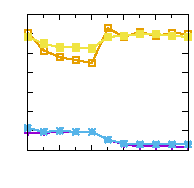
\includegraphics{plot_paper_decode_16bit_seq}}%
    \gplfronttext
  \end{picture}%
\endgroup

		\setcounter{subfigure}{2}
		\vspace{-3mm}
		\caption{Decode Scalar}
		\label{fig:codingbenchmark:decode:seq}%
	\end{subfigure}
	\hfill
	\begin{subfigure}[t]{1.3in}
		% GNUPLOT: LaTeX picture with Postscript
\begingroup
  \makeatletter
  \providecommand\color[2][]{%
    \GenericError{(gnuplot) \space\space\space\@spaces}{%
      Package color not loaded in conjunction with
      terminal option `colourtext'%
    }{See the gnuplot documentation for explanation.%
    }{Either use 'blacktext' in gnuplot or load the package
      color.sty in LaTeX.}%
    \renewcommand\color[2][]{}%
  }%
  \providecommand\includegraphics[2][]{%
    \GenericError{(gnuplot) \space\space\space\@spaces}{%
      Package graphicx or graphics not loaded%
    }{See the gnuplot documentation for explanation.%
    }{The gnuplot epslatex terminal needs graphicx.sty or graphics.sty.}%
    \renewcommand\includegraphics[2][]{}%
  }%
  \providecommand\rotatebox[2]{#2}%
  \@ifundefined{ifGPcolor}{%
    \newif\ifGPcolor
    \GPcolortrue
  }{}%
  \@ifundefined{ifGPblacktext}{%
    \newif\ifGPblacktext
    \GPblacktexttrue
  }{}%
  % define a \g@addto@macro without @ in the name:
  \let\gplgaddtomacro\g@addto@macro
  % define empty templates for all commands taking text:
  \gdef\gplbacktext{}%
  \gdef\gplfronttext{}%
  \makeatother
  \ifGPblacktext
    % no textcolor at all
    \def\colorrgb#1{}%
    \def\colorgray#1{}%
  \else
    % gray or color?
    \ifGPcolor
      \def\colorrgb#1{\color[rgb]{#1}}%
      \def\colorgray#1{\color[gray]{#1}}%
      \expandafter\def\csname LTw\endcsname{\color{white}}%
      \expandafter\def\csname LTb\endcsname{\color{black}}%
      \expandafter\def\csname LTa\endcsname{\color{black}}%
      \expandafter\def\csname LT0\endcsname{\color[rgb]{1,0,0}}%
      \expandafter\def\csname LT1\endcsname{\color[rgb]{0,1,0}}%
      \expandafter\def\csname LT2\endcsname{\color[rgb]{0,0,1}}%
      \expandafter\def\csname LT3\endcsname{\color[rgb]{1,0,1}}%
      \expandafter\def\csname LT4\endcsname{\color[rgb]{0,1,1}}%
      \expandafter\def\csname LT5\endcsname{\color[rgb]{1,1,0}}%
      \expandafter\def\csname LT6\endcsname{\color[rgb]{0,0,0}}%
      \expandafter\def\csname LT7\endcsname{\color[rgb]{1,0.3,0}}%
      \expandafter\def\csname LT8\endcsname{\color[rgb]{0.5,0.5,0.5}}%
    \else
      % gray
      \def\colorrgb#1{\color{black}}%
      \def\colorgray#1{\color[gray]{#1}}%
      \expandafter\def\csname LTw\endcsname{\color{white}}%
      \expandafter\def\csname LTb\endcsname{\color{black}}%
      \expandafter\def\csname LTa\endcsname{\color{black}}%
      \expandafter\def\csname LT0\endcsname{\color{black}}%
      \expandafter\def\csname LT1\endcsname{\color{black}}%
      \expandafter\def\csname LT2\endcsname{\color{black}}%
      \expandafter\def\csname LT3\endcsname{\color{black}}%
      \expandafter\def\csname LT4\endcsname{\color{black}}%
      \expandafter\def\csname LT5\endcsname{\color{black}}%
      \expandafter\def\csname LT6\endcsname{\color{black}}%
      \expandafter\def\csname LT7\endcsname{\color{black}}%
      \expandafter\def\csname LT8\endcsname{\color{black}}%
    \fi
  \fi
    \setlength{\unitlength}{0.0500bp}%
    \ifx\gptboxheight\undefined%
      \newlength{\gptboxheight}%
      \newlength{\gptboxwidth}%
      \newsavebox{\gptboxtext}%
    \fi%
    \setlength{\fboxrule}{0.5pt}%
    \setlength{\fboxsep}{1pt}%
\begin{picture}(1860.00,1800.00)%
    \gplgaddtomacro\gplbacktext{%
      \csname LTb\endcsname%
      \put(192,372){\makebox(0,0)[r]{\strut{}$0$}}%
      \csname LTb\endcsname%
      \put(192,502){\makebox(0,0)[r]{\strut{}$0.2$}}%
      \csname LTb\endcsname%
      \put(192,633){\makebox(0,0)[r]{\strut{}$0.4$}}%
      \csname LTb\endcsname%
      \put(192,763){\makebox(0,0)[r]{\strut{}$0.6$}}%
      \csname LTb\endcsname%
      \put(192,893){\makebox(0,0)[r]{\strut{}$0.8$}}%
      \csname LTb\endcsname%
      \put(192,1024){\makebox(0,0)[r]{\strut{}$1$}}%
      \csname LTb\endcsname%
      \put(192,1154){\makebox(0,0)[r]{\strut{}$1.2$}}%
      \csname LTb\endcsname%
      \put(192,1284){\makebox(0,0)[r]{\strut{}$1.4$}}%
      \csname LTb\endcsname%
      \put(192,1414){\makebox(0,0)[r]{\strut{}$1.6$}}%
      \csname LTb\endcsname%
      \put(192,1545){\makebox(0,0)[r]{\strut{}$1.8$}}%
      \csname LTb\endcsname%
      \put(192,1675){\makebox(0,0)[r]{\strut{}$2$}}%
      \csname LTb\endcsname%
      \put(256,248){\makebox(0,0){\strut{}$2^{0}$}}%
      \csname LTb\endcsname%
      \put(564,248){\makebox(0,0){\strut{}$2^{2}$}}%
      \csname LTb\endcsname%
      \put(872,248){\makebox(0,0){\strut{}$2^{4}$}}%
      \csname LTb\endcsname%
      \put(1179,248){\makebox(0,0){\strut{}$2^{6}$}}%
      \csname LTb\endcsname%
      \put(1487,248){\makebox(0,0){\strut{}$2^{8}$}}%
      \csname LTb\endcsname%
      \put(1795,248){\makebox(0,0){\strut{}$2^{10}$}}%
    }%
    \gplgaddtomacro\gplfronttext{%
      \csname LTb\endcsname%
      \put(1025,62){\makebox(0,0){\strut{}unroll / block size}}%
    }%
    \gplbacktext
    \put(0,0){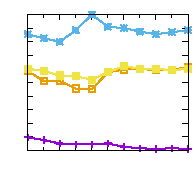
\includegraphics{plot_paper_check_16bit_seq}}%
    \gplfronttext
  \end{picture}%
\endgroup

		\setcounter{subfigure}{4}
		\vspace{-3mm}
		\caption{Detect Scalar}
		\label{fig:codingbenchmark:check:seq}%
	\end{subfigure}
	\hfill
	\begin{subfigure}[t]{1.3in}
		% GNUPLOT: LaTeX picture with Postscript
\begingroup
  \makeatletter
  \providecommand\color[2][]{%
    \GenericError{(gnuplot) \space\space\space\@spaces}{%
      Package color not loaded in conjunction with
      terminal option `colourtext'%
    }{See the gnuplot documentation for explanation.%
    }{Either use 'blacktext' in gnuplot or load the package
      color.sty in LaTeX.}%
    \renewcommand\color[2][]{}%
  }%
  \providecommand\includegraphics[2][]{%
    \GenericError{(gnuplot) \space\space\space\@spaces}{%
      Package graphicx or graphics not loaded%
    }{See the gnuplot documentation for explanation.%
    }{The gnuplot epslatex terminal needs graphicx.sty or graphics.sty.}%
    \renewcommand\includegraphics[2][]{}%
  }%
  \providecommand\rotatebox[2]{#2}%
  \@ifundefined{ifGPcolor}{%
    \newif\ifGPcolor
    \GPcolortrue
  }{}%
  \@ifundefined{ifGPblacktext}{%
    \newif\ifGPblacktext
    \GPblacktexttrue
  }{}%
  % define a \g@addto@macro without @ in the name:
  \let\gplgaddtomacro\g@addto@macro
  % define empty templates for all commands taking text:
  \gdef\gplbacktext{}%
  \gdef\gplfronttext{}%
  \makeatother
  \ifGPblacktext
    % no textcolor at all
    \def\colorrgb#1{}%
    \def\colorgray#1{}%
  \else
    % gray or color?
    \ifGPcolor
      \def\colorrgb#1{\color[rgb]{#1}}%
      \def\colorgray#1{\color[gray]{#1}}%
      \expandafter\def\csname LTw\endcsname{\color{white}}%
      \expandafter\def\csname LTb\endcsname{\color{black}}%
      \expandafter\def\csname LTa\endcsname{\color{black}}%
      \expandafter\def\csname LT0\endcsname{\color[rgb]{1,0,0}}%
      \expandafter\def\csname LT1\endcsname{\color[rgb]{0,1,0}}%
      \expandafter\def\csname LT2\endcsname{\color[rgb]{0,0,1}}%
      \expandafter\def\csname LT3\endcsname{\color[rgb]{1,0,1}}%
      \expandafter\def\csname LT4\endcsname{\color[rgb]{0,1,1}}%
      \expandafter\def\csname LT5\endcsname{\color[rgb]{1,1,0}}%
      \expandafter\def\csname LT6\endcsname{\color[rgb]{0,0,0}}%
      \expandafter\def\csname LT7\endcsname{\color[rgb]{1,0.3,0}}%
      \expandafter\def\csname LT8\endcsname{\color[rgb]{0.5,0.5,0.5}}%
    \else
      % gray
      \def\colorrgb#1{\color{black}}%
      \def\colorgray#1{\color[gray]{#1}}%
      \expandafter\def\csname LTw\endcsname{\color{white}}%
      \expandafter\def\csname LTb\endcsname{\color{black}}%
      \expandafter\def\csname LTa\endcsname{\color{black}}%
      \expandafter\def\csname LT0\endcsname{\color{black}}%
      \expandafter\def\csname LT1\endcsname{\color{black}}%
      \expandafter\def\csname LT2\endcsname{\color{black}}%
      \expandafter\def\csname LT3\endcsname{\color{black}}%
      \expandafter\def\csname LT4\endcsname{\color{black}}%
      \expandafter\def\csname LT5\endcsname{\color{black}}%
      \expandafter\def\csname LT6\endcsname{\color{black}}%
      \expandafter\def\csname LT7\endcsname{\color{black}}%
      \expandafter\def\csname LT8\endcsname{\color{black}}%
    \fi
  \fi
    \setlength{\unitlength}{0.0500bp}%
    \ifx\gptboxheight\undefined%
      \newlength{\gptboxheight}%
      \newlength{\gptboxwidth}%
      \newsavebox{\gptboxtext}%
    \fi%
    \setlength{\fboxrule}{0.5pt}%
    \setlength{\fboxsep}{1pt}%
\begin{picture}(1860.00,1800.00)%
    \gplgaddtomacro\gplbacktext{%
      \csname LTb\endcsname%
      \put(192,372){\makebox(0,0)[r]{\strut{}$0$}}%
      \csname LTb\endcsname%
      \put(192,535){\makebox(0,0)[r]{\strut{}$0.05$}}%
      \csname LTb\endcsname%
      \put(192,698){\makebox(0,0)[r]{\strut{}$0.1$}}%
      \csname LTb\endcsname%
      \put(192,861){\makebox(0,0)[r]{\strut{}$0.15$}}%
      \csname LTb\endcsname%
      \put(192,1024){\makebox(0,0)[r]{\strut{}$0.2$}}%
      \csname LTb\endcsname%
      \put(192,1186){\makebox(0,0)[r]{\strut{}$0.25$}}%
      \csname LTb\endcsname%
      \put(192,1349){\makebox(0,0)[r]{\strut{}$0.3$}}%
      \csname LTb\endcsname%
      \put(192,1512){\makebox(0,0)[r]{\strut{}$0.35$}}%
      \csname LTb\endcsname%
      \put(192,1675){\makebox(0,0)[r]{\strut{}$0.4$}}%
      \csname LTb\endcsname%
      \put(256,248){\makebox(0,0){\strut{}$2^{0}$}}%
      \csname LTb\endcsname%
      \put(564,248){\makebox(0,0){\strut{}$2^{2}$}}%
      \csname LTb\endcsname%
      \put(872,248){\makebox(0,0){\strut{}$2^{4}$}}%
      \csname LTb\endcsname%
      \put(1179,248){\makebox(0,0){\strut{}$2^{6}$}}%
      \csname LTb\endcsname%
      \put(1487,248){\makebox(0,0){\strut{}$2^{8}$}}%
      \csname LTb\endcsname%
      \put(1795,248){\makebox(0,0){\strut{}$2^{10}$}}%
    }%
    \gplgaddtomacro\gplfronttext{%
      \csname LTb\endcsname%
      \put(1025,62){\makebox(0,0){\strut{}unroll / block size}}%
    }%
    \gplbacktext
    \put(0,0){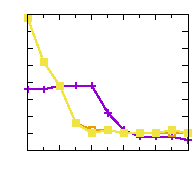
\includegraphics{plot_paper_decode_16bit_seq_inv}}%
    \gplfronttext
  \end{picture}%
\endgroup

		\setcounter{subfigure}{6}
		\vspace{-3mm}
		\caption{Refined Decode Scalar}
		\label{fig:refinements:decode:seq:zoom}
	\end{subfigure}
	\hfill
	\begin{subfigure}[t]{1.3in}
		% GNUPLOT: LaTeX picture with Postscript
\begingroup
  \makeatletter
  \providecommand\color[2][]{%
    \GenericError{(gnuplot) \space\space\space\@spaces}{%
      Package color not loaded in conjunction with
      terminal option `colourtext'%
    }{See the gnuplot documentation for explanation.%
    }{Either use 'blacktext' in gnuplot or load the package
      color.sty in LaTeX.}%
    \renewcommand\color[2][]{}%
  }%
  \providecommand\includegraphics[2][]{%
    \GenericError{(gnuplot) \space\space\space\@spaces}{%
      Package graphicx or graphics not loaded%
    }{See the gnuplot documentation for explanation.%
    }{The gnuplot epslatex terminal needs graphicx.sty or graphics.sty.}%
    \renewcommand\includegraphics[2][]{}%
  }%
  \providecommand\rotatebox[2]{#2}%
  \@ifundefined{ifGPcolor}{%
    \newif\ifGPcolor
    \GPcolortrue
  }{}%
  \@ifundefined{ifGPblacktext}{%
    \newif\ifGPblacktext
    \GPblacktexttrue
  }{}%
  % define a \g@addto@macro without @ in the name:
  \let\gplgaddtomacro\g@addto@macro
  % define empty templates for all commands taking text:
  \gdef\gplbacktext{}%
  \gdef\gplfronttext{}%
  \makeatother
  \ifGPblacktext
    % no textcolor at all
    \def\colorrgb#1{}%
    \def\colorgray#1{}%
  \else
    % gray or color?
    \ifGPcolor
      \def\colorrgb#1{\color[rgb]{#1}}%
      \def\colorgray#1{\color[gray]{#1}}%
      \expandafter\def\csname LTw\endcsname{\color{white}}%
      \expandafter\def\csname LTb\endcsname{\color{black}}%
      \expandafter\def\csname LTa\endcsname{\color{black}}%
      \expandafter\def\csname LT0\endcsname{\color[rgb]{1,0,0}}%
      \expandafter\def\csname LT1\endcsname{\color[rgb]{0,1,0}}%
      \expandafter\def\csname LT2\endcsname{\color[rgb]{0,0,1}}%
      \expandafter\def\csname LT3\endcsname{\color[rgb]{1,0,1}}%
      \expandafter\def\csname LT4\endcsname{\color[rgb]{0,1,1}}%
      \expandafter\def\csname LT5\endcsname{\color[rgb]{1,1,0}}%
      \expandafter\def\csname LT6\endcsname{\color[rgb]{0,0,0}}%
      \expandafter\def\csname LT7\endcsname{\color[rgb]{1,0.3,0}}%
      \expandafter\def\csname LT8\endcsname{\color[rgb]{0.5,0.5,0.5}}%
    \else
      % gray
      \def\colorrgb#1{\color{black}}%
      \def\colorgray#1{\color[gray]{#1}}%
      \expandafter\def\csname LTw\endcsname{\color{white}}%
      \expandafter\def\csname LTb\endcsname{\color{black}}%
      \expandafter\def\csname LTa\endcsname{\color{black}}%
      \expandafter\def\csname LT0\endcsname{\color{black}}%
      \expandafter\def\csname LT1\endcsname{\color{black}}%
      \expandafter\def\csname LT2\endcsname{\color{black}}%
      \expandafter\def\csname LT3\endcsname{\color{black}}%
      \expandafter\def\csname LT4\endcsname{\color{black}}%
      \expandafter\def\csname LT5\endcsname{\color{black}}%
      \expandafter\def\csname LT6\endcsname{\color{black}}%
      \expandafter\def\csname LT7\endcsname{\color{black}}%
      \expandafter\def\csname LT8\endcsname{\color{black}}%
    \fi
  \fi
    \setlength{\unitlength}{0.0500bp}%
    \ifx\gptboxheight\undefined%
      \newlength{\gptboxheight}%
      \newlength{\gptboxwidth}%
      \newsavebox{\gptboxtext}%
    \fi%
    \setlength{\fboxrule}{0.5pt}%
    \setlength{\fboxsep}{1pt}%
\begin{picture}(1860.00,1800.00)%
    \gplgaddtomacro\gplbacktext{%
      \csname LTb\endcsname%
      \put(192,372){\makebox(0,0)[r]{\strut{}$0$}}%
      \csname LTb\endcsname%
      \put(192,535){\makebox(0,0)[r]{\strut{}$0.05$}}%
      \csname LTb\endcsname%
      \put(192,698){\makebox(0,0)[r]{\strut{}$0.1$}}%
      \csname LTb\endcsname%
      \put(192,861){\makebox(0,0)[r]{\strut{}$0.15$}}%
      \csname LTb\endcsname%
      \put(192,1024){\makebox(0,0)[r]{\strut{}$0.2$}}%
      \csname LTb\endcsname%
      \put(192,1186){\makebox(0,0)[r]{\strut{}$0.25$}}%
      \csname LTb\endcsname%
      \put(192,1349){\makebox(0,0)[r]{\strut{}$0.3$}}%
      \csname LTb\endcsname%
      \put(192,1512){\makebox(0,0)[r]{\strut{}$0.35$}}%
      \csname LTb\endcsname%
      \put(192,1675){\makebox(0,0)[r]{\strut{}$0.4$}}%
      \csname LTb\endcsname%
      \put(256,248){\makebox(0,0){\strut{}$2^{0}$}}%
      \csname LTb\endcsname%
      \put(564,248){\makebox(0,0){\strut{}$2^{2}$}}%
      \csname LTb\endcsname%
      \put(872,248){\makebox(0,0){\strut{}$2^{4}$}}%
      \csname LTb\endcsname%
      \put(1179,248){\makebox(0,0){\strut{}$2^{6}$}}%
      \csname LTb\endcsname%
      \put(1487,248){\makebox(0,0){\strut{}$2^{8}$}}%
      \csname LTb\endcsname%
      \put(1795,248){\makebox(0,0){\strut{}$2^{10}$}}%
    }%
    \gplgaddtomacro\gplfronttext{%
      \csname LTb\endcsname%
      \put(1025,62){\makebox(0,0){\strut{}unroll / block size}}%
    }%
    \gplbacktext
    \put(0,0){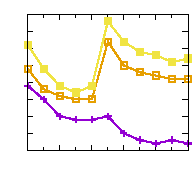
\includegraphics{plot_paper_check_16bit_seq_inv}}%
    \gplfronttext
  \end{picture}%
\endgroup

		\setcounter{subfigure}{8}
		\vspace{-3mm}
		\caption{Refined Detect Scalar}
		\label{fig:refinements:check:seq:zoom}
	\end{subfigure}
	\hfill\null
	\\
	\null\hfill
	\begin{subfigure}[t]{0.2in}
		% GNUPLOT: LaTeX picture with Postscript
\begingroup
  \makeatletter
  \providecommand\color[2][]{%
    \GenericError{(gnuplot) \space\space\space\@spaces}{%
      Package color not loaded in conjunction with
      terminal option `colourtext'%
    }{See the gnuplot documentation for explanation.%
    }{Either use 'blacktext' in gnuplot or load the package
      color.sty in LaTeX.}%
    \renewcommand\color[2][]{}%
  }%
  \providecommand\includegraphics[2][]{%
    \GenericError{(gnuplot) \space\space\space\@spaces}{%
      Package graphicx or graphics not loaded%
    }{See the gnuplot documentation for explanation.%
    }{The gnuplot epslatex terminal needs graphicx.sty or graphics.sty.}%
    \renewcommand\includegraphics[2][]{}%
  }%
  \providecommand\rotatebox[2]{#2}%
  \@ifundefined{ifGPcolor}{%
    \newif\ifGPcolor
    \GPcolortrue
  }{}%
  \@ifundefined{ifGPblacktext}{%
    \newif\ifGPblacktext
    \GPblacktexttrue
  }{}%
  % define a \g@addto@macro without @ in the name:
  \let\gplgaddtomacro\g@addto@macro
  % define empty templates for all commands taking text:
  \gdef\gplbacktext{}%
  \gdef\gplfronttext{}%
  \makeatother
  \ifGPblacktext
    % no textcolor at all
    \def\colorrgb#1{}%
    \def\colorgray#1{}%
  \else
    % gray or color?
    \ifGPcolor
      \def\colorrgb#1{\color[rgb]{#1}}%
      \def\colorgray#1{\color[gray]{#1}}%
      \expandafter\def\csname LTw\endcsname{\color{white}}%
      \expandafter\def\csname LTb\endcsname{\color{black}}%
      \expandafter\def\csname LTa\endcsname{\color{black}}%
      \expandafter\def\csname LT0\endcsname{\color[rgb]{1,0,0}}%
      \expandafter\def\csname LT1\endcsname{\color[rgb]{0,1,0}}%
      \expandafter\def\csname LT2\endcsname{\color[rgb]{0,0,1}}%
      \expandafter\def\csname LT3\endcsname{\color[rgb]{1,0,1}}%
      \expandafter\def\csname LT4\endcsname{\color[rgb]{0,1,1}}%
      \expandafter\def\csname LT5\endcsname{\color[rgb]{1,1,0}}%
      \expandafter\def\csname LT6\endcsname{\color[rgb]{0,0,0}}%
      \expandafter\def\csname LT7\endcsname{\color[rgb]{1,0.3,0}}%
      \expandafter\def\csname LT8\endcsname{\color[rgb]{0.5,0.5,0.5}}%
    \else
      % gray
      \def\colorrgb#1{\color{black}}%
      \def\colorgray#1{\color[gray]{#1}}%
      \expandafter\def\csname LTw\endcsname{\color{white}}%
      \expandafter\def\csname LTb\endcsname{\color{black}}%
      \expandafter\def\csname LTa\endcsname{\color{black}}%
      \expandafter\def\csname LT0\endcsname{\color{black}}%
      \expandafter\def\csname LT1\endcsname{\color{black}}%
      \expandafter\def\csname LT2\endcsname{\color{black}}%
      \expandafter\def\csname LT3\endcsname{\color{black}}%
      \expandafter\def\csname LT4\endcsname{\color{black}}%
      \expandafter\def\csname LT5\endcsname{\color{black}}%
      \expandafter\def\csname LT6\endcsname{\color{black}}%
      \expandafter\def\csname LT7\endcsname{\color{black}}%
      \expandafter\def\csname LT8\endcsname{\color{black}}%
    \fi
  \fi
    \setlength{\unitlength}{0.0500bp}%
    \ifx\gptboxheight\undefined%
      \newlength{\gptboxheight}%
      \newlength{\gptboxwidth}%
      \newsavebox{\gptboxtext}%
    \fi%
    \setlength{\fboxrule}{0.5pt}%
    \setlength{\fboxsep}{1pt}%
\begin{picture}(280.00,1800.00)%
    \gplgaddtomacro\gplbacktext{%
      \csname LTb\endcsname%
      \put(167,621){\rotatebox{90}{\makebox(0,0)[l]{\strut{}SSE Runtime [s]}}}%
    }%
    \gplgaddtomacro\gplfronttext{%
    }%
    \gplbacktext
    \put(0,0){
\includegraphics{plot_paper_ylabel_vectorized}}%
    \gplfronttext
  \end{picture}%
\endgroup

	\end{subfigure}
	\hfill
	\begin{subfigure}[t]{1.3in}
		% GNUPLOT: LaTeX picture with Postscript
\begingroup
  \makeatletter
  \providecommand\color[2][]{%
    \GenericError{(gnuplot) \space\space\space\@spaces}{%
      Package color not loaded in conjunction with
      terminal option `colourtext'%
    }{See the gnuplot documentation for explanation.%
    }{Either use 'blacktext' in gnuplot or load the package
      color.sty in LaTeX.}%
    \renewcommand\color[2][]{}%
  }%
  \providecommand\includegraphics[2][]{%
    \GenericError{(gnuplot) \space\space\space\@spaces}{%
      Package graphicx or graphics not loaded%
    }{See the gnuplot documentation for explanation.%
    }{The gnuplot epslatex terminal needs graphicx.sty or graphics.sty.}%
    \renewcommand\includegraphics[2][]{}%
  }%
  \providecommand\rotatebox[2]{#2}%
  \@ifundefined{ifGPcolor}{%
    \newif\ifGPcolor
    \GPcolortrue
  }{}%
  \@ifundefined{ifGPblacktext}{%
    \newif\ifGPblacktext
    \GPblacktexttrue
  }{}%
  % define a \g@addto@macro without @ in the name:
  \let\gplgaddtomacro\g@addto@macro
  % define empty templates for all commands taking text:
  \gdef\gplbacktext{}%
  \gdef\gplfronttext{}%
  \makeatother
  \ifGPblacktext
    % no textcolor at all
    \def\colorrgb#1{}%
    \def\colorgray#1{}%
  \else
    % gray or color?
    \ifGPcolor
      \def\colorrgb#1{\color[rgb]{#1}}%
      \def\colorgray#1{\color[gray]{#1}}%
      \expandafter\def\csname LTw\endcsname{\color{white}}%
      \expandafter\def\csname LTb\endcsname{\color{black}}%
      \expandafter\def\csname LTa\endcsname{\color{black}}%
      \expandafter\def\csname LT0\endcsname{\color[rgb]{1,0,0}}%
      \expandafter\def\csname LT1\endcsname{\color[rgb]{0,1,0}}%
      \expandafter\def\csname LT2\endcsname{\color[rgb]{0,0,1}}%
      \expandafter\def\csname LT3\endcsname{\color[rgb]{1,0,1}}%
      \expandafter\def\csname LT4\endcsname{\color[rgb]{0,1,1}}%
      \expandafter\def\csname LT5\endcsname{\color[rgb]{1,1,0}}%
      \expandafter\def\csname LT6\endcsname{\color[rgb]{0,0,0}}%
      \expandafter\def\csname LT7\endcsname{\color[rgb]{1,0.3,0}}%
      \expandafter\def\csname LT8\endcsname{\color[rgb]{0.5,0.5,0.5}}%
    \else
      % gray
      \def\colorrgb#1{\color{black}}%
      \def\colorgray#1{\color[gray]{#1}}%
      \expandafter\def\csname LTw\endcsname{\color{white}}%
      \expandafter\def\csname LTb\endcsname{\color{black}}%
      \expandafter\def\csname LTa\endcsname{\color{black}}%
      \expandafter\def\csname LT0\endcsname{\color{black}}%
      \expandafter\def\csname LT1\endcsname{\color{black}}%
      \expandafter\def\csname LT2\endcsname{\color{black}}%
      \expandafter\def\csname LT3\endcsname{\color{black}}%
      \expandafter\def\csname LT4\endcsname{\color{black}}%
      \expandafter\def\csname LT5\endcsname{\color{black}}%
      \expandafter\def\csname LT6\endcsname{\color{black}}%
      \expandafter\def\csname LT7\endcsname{\color{black}}%
      \expandafter\def\csname LT8\endcsname{\color{black}}%
    \fi
  \fi
    \setlength{\unitlength}{0.0500bp}%
    \ifx\gptboxheight\undefined%
      \newlength{\gptboxheight}%
      \newlength{\gptboxwidth}%
      \newsavebox{\gptboxtext}%
    \fi%
    \setlength{\fboxrule}{0.5pt}%
    \setlength{\fboxsep}{1pt}%
\begin{picture}(1860.00,1800.00)%
    \gplgaddtomacro\gplbacktext{%
      \csname LTb\endcsname%
      \put(192,372){\makebox(0,0)[r]{\strut{}$0$}}%
      \csname LTb\endcsname%
      \put(192,535){\makebox(0,0)[r]{\strut{}$0.2$}}%
      \csname LTb\endcsname%
      \put(192,698){\makebox(0,0)[r]{\strut{}$0.4$}}%
      \csname LTb\endcsname%
      \put(192,861){\makebox(0,0)[r]{\strut{}$0.6$}}%
      \csname LTb\endcsname%
      \put(192,1024){\makebox(0,0)[r]{\strut{}$0.8$}}%
      \csname LTb\endcsname%
      \put(192,1186){\makebox(0,0)[r]{\strut{}$1$}}%
      \csname LTb\endcsname%
      \put(192,1349){\makebox(0,0)[r]{\strut{}$1.2$}}%
      \csname LTb\endcsname%
      \put(192,1512){\makebox(0,0)[r]{\strut{}$1.4$}}%
      \csname LTb\endcsname%
      \put(192,1675){\makebox(0,0)[r]{\strut{}$1.6$}}%
      \csname LTb\endcsname%
      \put(256,248){\makebox(0,0){\strut{}$2^{0}$}}%
      \csname LTb\endcsname%
      \put(564,248){\makebox(0,0){\strut{}$2^{2}$}}%
      \csname LTb\endcsname%
      \put(872,248){\makebox(0,0){\strut{}$2^{4}$}}%
      \csname LTb\endcsname%
      \put(1179,248){\makebox(0,0){\strut{}$2^{6}$}}%
      \csname LTb\endcsname%
      \put(1487,248){\makebox(0,0){\strut{}$2^{8}$}}%
      \csname LTb\endcsname%
      \put(1795,248){\makebox(0,0){\strut{}$2^{10}$}}%
    }%
    \gplgaddtomacro\gplfronttext{%
      \csname LTb\endcsname%
      \put(1025,62){\makebox(0,0){\strut{}unroll / block size}}%
    }%
    \gplbacktext
    \put(0,0){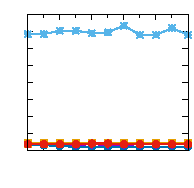
\includegraphics{plot_paper_encode_16bit_vec}}%
    \gplfronttext
  \end{picture}%
\endgroup

		\setcounter{subfigure}{1}
		\vspace{-3mm}
		\caption{Encode SSE4.2 / AVX2}
		\label{fig:codingbenchmark:hardening:vec}
	\end{subfigure}
	\hfill
	\begin{subfigure}[t]{1.3in}
		% GNUPLOT: LaTeX picture with Postscript
\begingroup
  \makeatletter
  \providecommand\color[2][]{%
    \GenericError{(gnuplot) \space\space\space\@spaces}{%
      Package color not loaded in conjunction with
      terminal option `colourtext'%
    }{See the gnuplot documentation for explanation.%
    }{Either use 'blacktext' in gnuplot or load the package
      color.sty in LaTeX.}%
    \renewcommand\color[2][]{}%
  }%
  \providecommand\includegraphics[2][]{%
    \GenericError{(gnuplot) \space\space\space\@spaces}{%
      Package graphicx or graphics not loaded%
    }{See the gnuplot documentation for explanation.%
    }{The gnuplot epslatex terminal needs graphicx.sty or graphics.sty.}%
    \renewcommand\includegraphics[2][]{}%
  }%
  \providecommand\rotatebox[2]{#2}%
  \@ifundefined{ifGPcolor}{%
    \newif\ifGPcolor
    \GPcolortrue
  }{}%
  \@ifundefined{ifGPblacktext}{%
    \newif\ifGPblacktext
    \GPblacktexttrue
  }{}%
  % define a \g@addto@macro without @ in the name:
  \let\gplgaddtomacro\g@addto@macro
  % define empty templates for all commands taking text:
  \gdef\gplbacktext{}%
  \gdef\gplfronttext{}%
  \makeatother
  \ifGPblacktext
    % no textcolor at all
    \def\colorrgb#1{}%
    \def\colorgray#1{}%
  \else
    % gray or color?
    \ifGPcolor
      \def\colorrgb#1{\color[rgb]{#1}}%
      \def\colorgray#1{\color[gray]{#1}}%
      \expandafter\def\csname LTw\endcsname{\color{white}}%
      \expandafter\def\csname LTb\endcsname{\color{black}}%
      \expandafter\def\csname LTa\endcsname{\color{black}}%
      \expandafter\def\csname LT0\endcsname{\color[rgb]{1,0,0}}%
      \expandafter\def\csname LT1\endcsname{\color[rgb]{0,1,0}}%
      \expandafter\def\csname LT2\endcsname{\color[rgb]{0,0,1}}%
      \expandafter\def\csname LT3\endcsname{\color[rgb]{1,0,1}}%
      \expandafter\def\csname LT4\endcsname{\color[rgb]{0,1,1}}%
      \expandafter\def\csname LT5\endcsname{\color[rgb]{1,1,0}}%
      \expandafter\def\csname LT6\endcsname{\color[rgb]{0,0,0}}%
      \expandafter\def\csname LT7\endcsname{\color[rgb]{1,0.3,0}}%
      \expandafter\def\csname LT8\endcsname{\color[rgb]{0.5,0.5,0.5}}%
    \else
      % gray
      \def\colorrgb#1{\color{black}}%
      \def\colorgray#1{\color[gray]{#1}}%
      \expandafter\def\csname LTw\endcsname{\color{white}}%
      \expandafter\def\csname LTb\endcsname{\color{black}}%
      \expandafter\def\csname LTa\endcsname{\color{black}}%
      \expandafter\def\csname LT0\endcsname{\color{black}}%
      \expandafter\def\csname LT1\endcsname{\color{black}}%
      \expandafter\def\csname LT2\endcsname{\color{black}}%
      \expandafter\def\csname LT3\endcsname{\color{black}}%
      \expandafter\def\csname LT4\endcsname{\color{black}}%
      \expandafter\def\csname LT5\endcsname{\color{black}}%
      \expandafter\def\csname LT6\endcsname{\color{black}}%
      \expandafter\def\csname LT7\endcsname{\color{black}}%
      \expandafter\def\csname LT8\endcsname{\color{black}}%
    \fi
  \fi
    \setlength{\unitlength}{0.0500bp}%
    \ifx\gptboxheight\undefined%
      \newlength{\gptboxheight}%
      \newlength{\gptboxwidth}%
      \newsavebox{\gptboxtext}%
    \fi%
    \setlength{\fboxrule}{0.5pt}%
    \setlength{\fboxsep}{1pt}%
\begin{picture}(1860.00,1800.00)%
    \gplgaddtomacro\gplbacktext{%
      \csname LTb\endcsname%
      \put(192,372){\makebox(0,0)[r]{\strut{}$0$}}%
      \csname LTb\endcsname%
      \put(192,558){\makebox(0,0)[r]{\strut{}$0.05$}}%
      \csname LTb\endcsname%
      \put(192,744){\makebox(0,0)[r]{\strut{}$0.1$}}%
      \csname LTb\endcsname%
      \put(192,930){\makebox(0,0)[r]{\strut{}$0.15$}}%
      \csname LTb\endcsname%
      \put(192,1117){\makebox(0,0)[r]{\strut{}$0.2$}}%
      \csname LTb\endcsname%
      \put(192,1303){\makebox(0,0)[r]{\strut{}$0.25$}}%
      \csname LTb\endcsname%
      \put(192,1489){\makebox(0,0)[r]{\strut{}$0.3$}}%
      \csname LTb\endcsname%
      \put(192,1675){\makebox(0,0)[r]{\strut{}$0.35$}}%
      \csname LTb\endcsname%
      \put(256,248){\makebox(0,0){\strut{}$2^{0}$}}%
      \csname LTb\endcsname%
      \put(564,248){\makebox(0,0){\strut{}$2^{2}$}}%
      \csname LTb\endcsname%
      \put(872,248){\makebox(0,0){\strut{}$2^{4}$}}%
      \csname LTb\endcsname%
      \put(1179,248){\makebox(0,0){\strut{}$2^{6}$}}%
      \csname LTb\endcsname%
      \put(1487,248){\makebox(0,0){\strut{}$2^{8}$}}%
      \csname LTb\endcsname%
      \put(1795,248){\makebox(0,0){\strut{}$2^{10}$}}%
    }%
    \gplgaddtomacro\gplfronttext{%
      \csname LTb\endcsname%
      \put(1025,62){\makebox(0,0){\strut{}unroll / block size}}%
    }%
    \gplbacktext
    \put(0,0){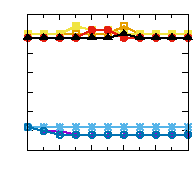
\includegraphics{plot_paper_decode_16bit_vec}}%
    \gplfronttext
  \end{picture}%
\endgroup

		\setcounter{subfigure}{3}
		\vspace{-3mm}
		\caption{Decode SSE4.2 / AVX2}
		\label{fig:codingbenchmark:decode:vec}%
	\end{subfigure}
	\hfill
	\begin{subfigure}[t]{1.3in}
		% GNUPLOT: LaTeX picture with Postscript
\begingroup
  \makeatletter
  \providecommand\color[2][]{%
    \GenericError{(gnuplot) \space\space\space\@spaces}{%
      Package color not loaded in conjunction with
      terminal option `colourtext'%
    }{See the gnuplot documentation for explanation.%
    }{Either use 'blacktext' in gnuplot or load the package
      color.sty in LaTeX.}%
    \renewcommand\color[2][]{}%
  }%
  \providecommand\includegraphics[2][]{%
    \GenericError{(gnuplot) \space\space\space\@spaces}{%
      Package graphicx or graphics not loaded%
    }{See the gnuplot documentation for explanation.%
    }{The gnuplot epslatex terminal needs graphicx.sty or graphics.sty.}%
    \renewcommand\includegraphics[2][]{}%
  }%
  \providecommand\rotatebox[2]{#2}%
  \@ifundefined{ifGPcolor}{%
    \newif\ifGPcolor
    \GPcolortrue
  }{}%
  \@ifundefined{ifGPblacktext}{%
    \newif\ifGPblacktext
    \GPblacktexttrue
  }{}%
  % define a \g@addto@macro without @ in the name:
  \let\gplgaddtomacro\g@addto@macro
  % define empty templates for all commands taking text:
  \gdef\gplbacktext{}%
  \gdef\gplfronttext{}%
  \makeatother
  \ifGPblacktext
    % no textcolor at all
    \def\colorrgb#1{}%
    \def\colorgray#1{}%
  \else
    % gray or color?
    \ifGPcolor
      \def\colorrgb#1{\color[rgb]{#1}}%
      \def\colorgray#1{\color[gray]{#1}}%
      \expandafter\def\csname LTw\endcsname{\color{white}}%
      \expandafter\def\csname LTb\endcsname{\color{black}}%
      \expandafter\def\csname LTa\endcsname{\color{black}}%
      \expandafter\def\csname LT0\endcsname{\color[rgb]{1,0,0}}%
      \expandafter\def\csname LT1\endcsname{\color[rgb]{0,1,0}}%
      \expandafter\def\csname LT2\endcsname{\color[rgb]{0,0,1}}%
      \expandafter\def\csname LT3\endcsname{\color[rgb]{1,0,1}}%
      \expandafter\def\csname LT4\endcsname{\color[rgb]{0,1,1}}%
      \expandafter\def\csname LT5\endcsname{\color[rgb]{1,1,0}}%
      \expandafter\def\csname LT6\endcsname{\color[rgb]{0,0,0}}%
      \expandafter\def\csname LT7\endcsname{\color[rgb]{1,0.3,0}}%
      \expandafter\def\csname LT8\endcsname{\color[rgb]{0.5,0.5,0.5}}%
    \else
      % gray
      \def\colorrgb#1{\color{black}}%
      \def\colorgray#1{\color[gray]{#1}}%
      \expandafter\def\csname LTw\endcsname{\color{white}}%
      \expandafter\def\csname LTb\endcsname{\color{black}}%
      \expandafter\def\csname LTa\endcsname{\color{black}}%
      \expandafter\def\csname LT0\endcsname{\color{black}}%
      \expandafter\def\csname LT1\endcsname{\color{black}}%
      \expandafter\def\csname LT2\endcsname{\color{black}}%
      \expandafter\def\csname LT3\endcsname{\color{black}}%
      \expandafter\def\csname LT4\endcsname{\color{black}}%
      \expandafter\def\csname LT5\endcsname{\color{black}}%
      \expandafter\def\csname LT6\endcsname{\color{black}}%
      \expandafter\def\csname LT7\endcsname{\color{black}}%
      \expandafter\def\csname LT8\endcsname{\color{black}}%
    \fi
  \fi
    \setlength{\unitlength}{0.0500bp}%
    \ifx\gptboxheight\undefined%
      \newlength{\gptboxheight}%
      \newlength{\gptboxwidth}%
      \newsavebox{\gptboxtext}%
    \fi%
    \setlength{\fboxrule}{0.5pt}%
    \setlength{\fboxsep}{1pt}%
\begin{picture}(1860.00,1800.00)%
    \gplgaddtomacro\gplbacktext{%
      \csname LTb\endcsname%
      \put(192,372){\makebox(0,0)[r]{\strut{}$0$}}%
      \csname LTb\endcsname%
      \put(192,535){\makebox(0,0)[r]{\strut{}$0.2$}}%
      \csname LTb\endcsname%
      \put(192,698){\makebox(0,0)[r]{\strut{}$0.4$}}%
      \csname LTb\endcsname%
      \put(192,861){\makebox(0,0)[r]{\strut{}$0.6$}}%
      \csname LTb\endcsname%
      \put(192,1024){\makebox(0,0)[r]{\strut{}$0.8$}}%
      \csname LTb\endcsname%
      \put(192,1186){\makebox(0,0)[r]{\strut{}$1$}}%
      \csname LTb\endcsname%
      \put(192,1349){\makebox(0,0)[r]{\strut{}$1.2$}}%
      \csname LTb\endcsname%
      \put(192,1512){\makebox(0,0)[r]{\strut{}$1.4$}}%
      \csname LTb\endcsname%
      \put(192,1675){\makebox(0,0)[r]{\strut{}$1.6$}}%
      \csname LTb\endcsname%
      \put(256,248){\makebox(0,0){\strut{}$2^{0}$}}%
      \csname LTb\endcsname%
      \put(564,248){\makebox(0,0){\strut{}$2^{2}$}}%
      \csname LTb\endcsname%
      \put(872,248){\makebox(0,0){\strut{}$2^{4}$}}%
      \csname LTb\endcsname%
      \put(1179,248){\makebox(0,0){\strut{}$2^{6}$}}%
      \csname LTb\endcsname%
      \put(1487,248){\makebox(0,0){\strut{}$2^{8}$}}%
      \csname LTb\endcsname%
      \put(1795,248){\makebox(0,0){\strut{}$2^{10}$}}%
    }%
    \gplgaddtomacro\gplfronttext{%
      \csname LTb\endcsname%
      \put(1025,62){\makebox(0,0){\strut{}unroll / block size}}%
    }%
    \gplbacktext
    \put(0,0){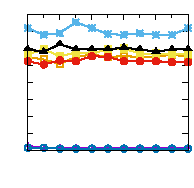
\includegraphics{plot_paper_check_16bit_vec}}%
    \gplfronttext
  \end{picture}%
\endgroup

		\setcounter{subfigure}{5}
		\vspace{-3mm}
		\caption{Detect SSE4.2 / AVX2}
		\label{fig:codingbenchmark:check:vec}%
	\end{subfigure}
	\hfill
	\begin{subfigure}[t]{1.3in}
		% GNUPLOT: LaTeX picture with Postscript
\begingroup
  \makeatletter
  \providecommand\color[2][]{%
    \GenericError{(gnuplot) \space\space\space\@spaces}{%
      Package color not loaded in conjunction with
      terminal option `colourtext'%
    }{See the gnuplot documentation for explanation.%
    }{Either use 'blacktext' in gnuplot or load the package
      color.sty in LaTeX.}%
    \renewcommand\color[2][]{}%
  }%
  \providecommand\includegraphics[2][]{%
    \GenericError{(gnuplot) \space\space\space\@spaces}{%
      Package graphicx or graphics not loaded%
    }{See the gnuplot documentation for explanation.%
    }{The gnuplot epslatex terminal needs graphicx.sty or graphics.sty.}%
    \renewcommand\includegraphics[2][]{}%
  }%
  \providecommand\rotatebox[2]{#2}%
  \@ifundefined{ifGPcolor}{%
    \newif\ifGPcolor
    \GPcolortrue
  }{}%
  \@ifundefined{ifGPblacktext}{%
    \newif\ifGPblacktext
    \GPblacktexttrue
  }{}%
  % define a \g@addto@macro without @ in the name:
  \let\gplgaddtomacro\g@addto@macro
  % define empty templates for all commands taking text:
  \gdef\gplbacktext{}%
  \gdef\gplfronttext{}%
  \makeatother
  \ifGPblacktext
    % no textcolor at all
    \def\colorrgb#1{}%
    \def\colorgray#1{}%
  \else
    % gray or color?
    \ifGPcolor
      \def\colorrgb#1{\color[rgb]{#1}}%
      \def\colorgray#1{\color[gray]{#1}}%
      \expandafter\def\csname LTw\endcsname{\color{white}}%
      \expandafter\def\csname LTb\endcsname{\color{black}}%
      \expandafter\def\csname LTa\endcsname{\color{black}}%
      \expandafter\def\csname LT0\endcsname{\color[rgb]{1,0,0}}%
      \expandafter\def\csname LT1\endcsname{\color[rgb]{0,1,0}}%
      \expandafter\def\csname LT2\endcsname{\color[rgb]{0,0,1}}%
      \expandafter\def\csname LT3\endcsname{\color[rgb]{1,0,1}}%
      \expandafter\def\csname LT4\endcsname{\color[rgb]{0,1,1}}%
      \expandafter\def\csname LT5\endcsname{\color[rgb]{1,1,0}}%
      \expandafter\def\csname LT6\endcsname{\color[rgb]{0,0,0}}%
      \expandafter\def\csname LT7\endcsname{\color[rgb]{1,0.3,0}}%
      \expandafter\def\csname LT8\endcsname{\color[rgb]{0.5,0.5,0.5}}%
    \else
      % gray
      \def\colorrgb#1{\color{black}}%
      \def\colorgray#1{\color[gray]{#1}}%
      \expandafter\def\csname LTw\endcsname{\color{white}}%
      \expandafter\def\csname LTb\endcsname{\color{black}}%
      \expandafter\def\csname LTa\endcsname{\color{black}}%
      \expandafter\def\csname LT0\endcsname{\color{black}}%
      \expandafter\def\csname LT1\endcsname{\color{black}}%
      \expandafter\def\csname LT2\endcsname{\color{black}}%
      \expandafter\def\csname LT3\endcsname{\color{black}}%
      \expandafter\def\csname LT4\endcsname{\color{black}}%
      \expandafter\def\csname LT5\endcsname{\color{black}}%
      \expandafter\def\csname LT6\endcsname{\color{black}}%
      \expandafter\def\csname LT7\endcsname{\color{black}}%
      \expandafter\def\csname LT8\endcsname{\color{black}}%
    \fi
  \fi
    \setlength{\unitlength}{0.0500bp}%
    \ifx\gptboxheight\undefined%
      \newlength{\gptboxheight}%
      \newlength{\gptboxwidth}%
      \newsavebox{\gptboxtext}%
    \fi%
    \setlength{\fboxrule}{0.5pt}%
    \setlength{\fboxsep}{1pt}%
\begin{picture}(1860.00,1800.00)%
    \gplgaddtomacro\gplbacktext{%
      \csname LTb\endcsname%
      \put(192,372){\makebox(0,0)[r]{\strut{}$0.02$}}%
      \csname LTb\endcsname%
      \put(192,589){\makebox(0,0)[r]{\strut{}$0.04$}}%
      \csname LTb\endcsname%
      \put(192,806){\makebox(0,0)[r]{\strut{}$0.06$}}%
      \csname LTb\endcsname%
      \put(192,1024){\makebox(0,0)[r]{\strut{}$0.08$}}%
      \csname LTb\endcsname%
      \put(192,1241){\makebox(0,0)[r]{\strut{}$0.1$}}%
      \csname LTb\endcsname%
      \put(192,1458){\makebox(0,0)[r]{\strut{}$0.12$}}%
      \csname LTb\endcsname%
      \put(192,1675){\makebox(0,0)[r]{\strut{}$0.14$}}%
      \csname LTb\endcsname%
      \put(256,248){\makebox(0,0){\strut{}$2^{0}$}}%
      \csname LTb\endcsname%
      \put(564,248){\makebox(0,0){\strut{}$2^{2}$}}%
      \csname LTb\endcsname%
      \put(872,248){\makebox(0,0){\strut{}$2^{4}$}}%
      \csname LTb\endcsname%
      \put(1179,248){\makebox(0,0){\strut{}$2^{6}$}}%
      \csname LTb\endcsname%
      \put(1487,248){\makebox(0,0){\strut{}$2^{8}$}}%
      \csname LTb\endcsname%
      \put(1795,248){\makebox(0,0){\strut{}$2^{10}$}}%
    }%
    \gplgaddtomacro\gplfronttext{%
      \csname LTb\endcsname%
      \put(1025,62){\makebox(0,0){\strut{}unroll / block size}}%
    }%
    \gplbacktext
    \put(0,0){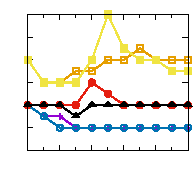
\includegraphics{plot_paper_decode_16bit_vec_inv}}%
    \gplfronttext
  \end{picture}%
\endgroup

		\setcounter{subfigure}{7}
		\vspace{-3mm}
		\caption{SSE4.2 / AVX2}
		\label{fig:refinements:decode:vec:zoom}
	\end{subfigure}
	\hfill
	\begin{subfigure}[t]{1.3in}
		% GNUPLOT: LaTeX picture with Postscript
\begingroup
  \makeatletter
  \providecommand\color[2][]{%
    \GenericError{(gnuplot) \space\space\space\@spaces}{%
      Package color not loaded in conjunction with
      terminal option `colourtext'%
    }{See the gnuplot documentation for explanation.%
    }{Either use 'blacktext' in gnuplot or load the package
      color.sty in LaTeX.}%
    \renewcommand\color[2][]{}%
  }%
  \providecommand\includegraphics[2][]{%
    \GenericError{(gnuplot) \space\space\space\@spaces}{%
      Package graphicx or graphics not loaded%
    }{See the gnuplot documentation for explanation.%
    }{The gnuplot epslatex terminal needs graphicx.sty or graphics.sty.}%
    \renewcommand\includegraphics[2][]{}%
  }%
  \providecommand\rotatebox[2]{#2}%
  \@ifundefined{ifGPcolor}{%
    \newif\ifGPcolor
    \GPcolortrue
  }{}%
  \@ifundefined{ifGPblacktext}{%
    \newif\ifGPblacktext
    \GPblacktexttrue
  }{}%
  % define a \g@addto@macro without @ in the name:
  \let\gplgaddtomacro\g@addto@macro
  % define empty templates for all commands taking text:
  \gdef\gplbacktext{}%
  \gdef\gplfronttext{}%
  \makeatother
  \ifGPblacktext
    % no textcolor at all
    \def\colorrgb#1{}%
    \def\colorgray#1{}%
  \else
    % gray or color?
    \ifGPcolor
      \def\colorrgb#1{\color[rgb]{#1}}%
      \def\colorgray#1{\color[gray]{#1}}%
      \expandafter\def\csname LTw\endcsname{\color{white}}%
      \expandafter\def\csname LTb\endcsname{\color{black}}%
      \expandafter\def\csname LTa\endcsname{\color{black}}%
      \expandafter\def\csname LT0\endcsname{\color[rgb]{1,0,0}}%
      \expandafter\def\csname LT1\endcsname{\color[rgb]{0,1,0}}%
      \expandafter\def\csname LT2\endcsname{\color[rgb]{0,0,1}}%
      \expandafter\def\csname LT3\endcsname{\color[rgb]{1,0,1}}%
      \expandafter\def\csname LT4\endcsname{\color[rgb]{0,1,1}}%
      \expandafter\def\csname LT5\endcsname{\color[rgb]{1,1,0}}%
      \expandafter\def\csname LT6\endcsname{\color[rgb]{0,0,0}}%
      \expandafter\def\csname LT7\endcsname{\color[rgb]{1,0.3,0}}%
      \expandafter\def\csname LT8\endcsname{\color[rgb]{0.5,0.5,0.5}}%
    \else
      % gray
      \def\colorrgb#1{\color{black}}%
      \def\colorgray#1{\color[gray]{#1}}%
      \expandafter\def\csname LTw\endcsname{\color{white}}%
      \expandafter\def\csname LTb\endcsname{\color{black}}%
      \expandafter\def\csname LTa\endcsname{\color{black}}%
      \expandafter\def\csname LT0\endcsname{\color{black}}%
      \expandafter\def\csname LT1\endcsname{\color{black}}%
      \expandafter\def\csname LT2\endcsname{\color{black}}%
      \expandafter\def\csname LT3\endcsname{\color{black}}%
      \expandafter\def\csname LT4\endcsname{\color{black}}%
      \expandafter\def\csname LT5\endcsname{\color{black}}%
      \expandafter\def\csname LT6\endcsname{\color{black}}%
      \expandafter\def\csname LT7\endcsname{\color{black}}%
      \expandafter\def\csname LT8\endcsname{\color{black}}%
    \fi
  \fi
    \setlength{\unitlength}{0.0500bp}%
    \ifx\gptboxheight\undefined%
      \newlength{\gptboxheight}%
      \newlength{\gptboxwidth}%
      \newsavebox{\gptboxtext}%
    \fi%
    \setlength{\fboxrule}{0.5pt}%
    \setlength{\fboxsep}{1pt}%
\begin{picture}(1860.00,1800.00)%
    \gplgaddtomacro\gplbacktext{%
      \csname LTb\endcsname%
      \put(192,372){\makebox(0,0)[r]{\strut{}$0$}}%
      \csname LTb\endcsname%
      \put(192,517){\makebox(0,0)[r]{\strut{}$0.02$}}%
      \csname LTb\endcsname%
      \put(192,662){\makebox(0,0)[r]{\strut{}$0.04$}}%
      \csname LTb\endcsname%
      \put(192,806){\makebox(0,0)[r]{\strut{}$0.06$}}%
      \csname LTb\endcsname%
      \put(192,951){\makebox(0,0)[r]{\strut{}$0.08$}}%
      \csname LTb\endcsname%
      \put(192,1096){\makebox(0,0)[r]{\strut{}$0.1$}}%
      \csname LTb\endcsname%
      \put(192,1241){\makebox(0,0)[r]{\strut{}$0.12$}}%
      \csname LTb\endcsname%
      \put(192,1385){\makebox(0,0)[r]{\strut{}$0.14$}}%
      \csname LTb\endcsname%
      \put(192,1530){\makebox(0,0)[r]{\strut{}$0.16$}}%
      \csname LTb\endcsname%
      \put(192,1675){\makebox(0,0)[r]{\strut{}$0.18$}}%
      \csname LTb\endcsname%
      \put(256,248){\makebox(0,0){\strut{}$2^{0}$}}%
      \csname LTb\endcsname%
      \put(564,248){\makebox(0,0){\strut{}$2^{2}$}}%
      \csname LTb\endcsname%
      \put(872,248){\makebox(0,0){\strut{}$2^{4}$}}%
      \csname LTb\endcsname%
      \put(1179,248){\makebox(0,0){\strut{}$2^{6}$}}%
      \csname LTb\endcsname%
      \put(1487,248){\makebox(0,0){\strut{}$2^{8}$}}%
      \csname LTb\endcsname%
      \put(1795,248){\makebox(0,0){\strut{}$2^{10}$}}%
    }%
    \gplgaddtomacro\gplfronttext{%
      \csname LTb\endcsname%
      \put(1025,62){\makebox(0,0){\strut{}unroll / block size}}%
    }%
    \gplbacktext
    \put(0,0){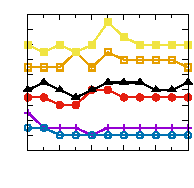
\includegraphics{plot_paper_check_16bit_vec_inv}}%
    \gplfronttext
  \end{picture}%
\endgroup

		\setcounter{subfigure}{9}
		\vspace{-3mm}
		\caption{SSE4.2 / AVX2}
		\label{fig:refinements:check:vec:zoom}
	\end{subfigure}
	\hfill\null
	\\
	\null\hfill
	% GNUPLOT: LaTeX picture with Postscript
\begingroup
  \makeatletter
  \providecommand\color[2][]{%
    \GenericError{(gnuplot) \space\space\space\@spaces}{%
      Package color not loaded in conjunction with
      terminal option `colourtext'%
    }{See the gnuplot documentation for explanation.%
    }{Either use 'blacktext' in gnuplot or load the package
      color.sty in LaTeX.}%
    \renewcommand\color[2][]{}%
  }%
  \providecommand\includegraphics[2][]{%
    \GenericError{(gnuplot) \space\space\space\@spaces}{%
      Package graphicx or graphics not loaded%
    }{See the gnuplot documentation for explanation.%
    }{The gnuplot epslatex terminal needs graphicx.sty or graphics.sty.}%
    \renewcommand\includegraphics[2][]{}%
  }%
  \providecommand\rotatebox[2]{#2}%
  \@ifundefined{ifGPcolor}{%
    \newif\ifGPcolor
    \GPcolortrue
  }{}%
  \@ifundefined{ifGPblacktext}{%
    \newif\ifGPblacktext
    \GPblacktexttrue
  }{}%
  % define a \g@addto@macro without @ in the name:
  \let\gplgaddtomacro\g@addto@macro
  % define empty templates for all commands taking text:
  \gdef\gplbacktext{}%
  \gdef\gplfronttext{}%
  \makeatother
  \ifGPblacktext
    % no textcolor at all
    \def\colorrgb#1{}%
    \def\colorgray#1{}%
  \else
    % gray or color?
    \ifGPcolor
      \def\colorrgb#1{\color[rgb]{#1}}%
      \def\colorgray#1{\color[gray]{#1}}%
      \expandafter\def\csname LTw\endcsname{\color{white}}%
      \expandafter\def\csname LTb\endcsname{\color{black}}%
      \expandafter\def\csname LTa\endcsname{\color{black}}%
      \expandafter\def\csname LT0\endcsname{\color[rgb]{1,0,0}}%
      \expandafter\def\csname LT1\endcsname{\color[rgb]{0,1,0}}%
      \expandafter\def\csname LT2\endcsname{\color[rgb]{0,0,1}}%
      \expandafter\def\csname LT3\endcsname{\color[rgb]{1,0,1}}%
      \expandafter\def\csname LT4\endcsname{\color[rgb]{0,1,1}}%
      \expandafter\def\csname LT5\endcsname{\color[rgb]{1,1,0}}%
      \expandafter\def\csname LT6\endcsname{\color[rgb]{0,0,0}}%
      \expandafter\def\csname LT7\endcsname{\color[rgb]{1,0.3,0}}%
      \expandafter\def\csname LT8\endcsname{\color[rgb]{0.5,0.5,0.5}}%
    \else
      % gray
      \def\colorrgb#1{\color{black}}%
      \def\colorgray#1{\color[gray]{#1}}%
      \expandafter\def\csname LTw\endcsname{\color{white}}%
      \expandafter\def\csname LTb\endcsname{\color{black}}%
      \expandafter\def\csname LTa\endcsname{\color{black}}%
      \expandafter\def\csname LT0\endcsname{\color{black}}%
      \expandafter\def\csname LT1\endcsname{\color{black}}%
      \expandafter\def\csname LT2\endcsname{\color{black}}%
      \expandafter\def\csname LT3\endcsname{\color{black}}%
      \expandafter\def\csname LT4\endcsname{\color{black}}%
      \expandafter\def\csname LT5\endcsname{\color{black}}%
      \expandafter\def\csname LT6\endcsname{\color{black}}%
      \expandafter\def\csname LT7\endcsname{\color{black}}%
      \expandafter\def\csname LT8\endcsname{\color{black}}%
    \fi
  \fi
    \setlength{\unitlength}{0.0500bp}%
    \ifx\gptboxheight\undefined%
      \newlength{\gptboxheight}%
      \newlength{\gptboxwidth}%
      \newsavebox{\gptboxtext}%
    \fi%
    \setlength{\fboxrule}{0.5pt}%
    \setlength{\fboxsep}{1pt}%
\begin{picture}(9360.00,560.00)%
    \gplgaddtomacro\gplbacktext{%
    }%
    \gplgaddtomacro\gplfronttext{%
      \csname LTb\endcsname%
      \put(2080,410){\makebox(0,0)[r]{\strut{}XOR$^{\text{scalar/SSE}}$}}%
      \csname LTb\endcsname%
      \put(2080,178){\makebox(0,0)[r]{\strut{}XOR$^{\text{AVX2}}$}}%
      \csname LTb\endcsname%
      \put(3942,410){\makebox(0,0)[r]{\strut{}AN$_{U}^{\text{scalar/SSE}}$}}%
      \csname LTb\endcsname%
      \put(3942,178){\makebox(0,0)[r]{\strut{}AN$_{S}^{\text{scalar/SSE}}$}}%
      \csname LTb\endcsname%
      \put(5804,410){\makebox(0,0)[r]{\strut{}AN$_{U}^{\text{AVX2}}$}}%
      \csname LTb\endcsname%
      \put(5804,178){\makebox(0,0)[r]{\strut{}AN$_{S}^{\text{AVX2}}$}}%
      \csname LTb\endcsname%
      \put(7666,410){\makebox(0,0)[r]{\strut{}Hamming}}%
    }%
    \gplbacktext
    \put(0,0){
\includegraphics{plot_paper_legend}}%
    \gplfronttext
  \end{picture}%
\endgroup

	\hfill\null
	\vspace{-4mm}
	\caption{Micro Benchmarks -- runtimes for scalar, SSE4.2 and AVX2 code functions. For XOR the block size is varied, while for Hamming and AN a loop unroll factor is varied. \(AN_U=\) unsigned, \(AN_S=\) signed.}%
	\label{fig:codingbenchmark:encode}%
	\vspace{-3mm}
\end{figure*}

\section{Mirco Benchmarks}
\label{sec:MicroBenchmarks}

We also conducted micro benchmarks to support our error code decision from a performance perspective. 

\subsection{Error Code Evaluation}

In our first micro benchmark series, we compared AN coding with other well-known und heavily applied coding schemes to show the advantages of AN coding for software-based error detection. In detail, we consider Hamming codes as presented in Section~\ref{sec:ErrorCoding} and checksums, both \emph{systematic error codes} where data bits and additional, redundant bits are separable. \emph{Checksums} add a small\=sized value derived from an arbitrary data block forming a hardened data block allowing limited error detection. Nowadays, the term checksum is also used when hash functions are applied. There exists a multitude of algorithms with varying complexity and hardware support, e.g. parity bits, parity words, Message\=Digest Algorithms (e.g. MD5)~\cite{md5,Sivathanu2005} or cyclic redundancy checks (e.g. CRC32)~\cite{peterson1961cyclic,Sivathanu2005}. In the case of parity bits (words), the data bits (words) are summed up using the binary exclusive or operation (XOR, \(\oplus\)). The size of the resulting checksum can be arbitrary, but is usually either a single bit or aligned to machine words, respectively, for the sake of performance. In the following, we restrict our discussion to XOR checksums, since they are one of the most simple types of checksums. Furthermore, both Hamming code and XOR checksum can be vectorized~\cite{mula2016avx2popcount,warren2013hacker} which is important for performance. 

In detail, we compared runtime overheads for the following functions: \emph{hardening}, \emph{decoding} and \emph{error detection}. For this, we implemented these functions for all three error codes using C++ template-meta programming to let the compiler unroll the code. We always implemented scalar and SSE4.2 variants, and AVX2 for AN and XOR. In the experiments, we processed about 250 Million 16\=bit integers depending on either the blocksize (XOR) or a loop unroll factor (AN, Hamming). The blocksize indicates over how many values a checksum is computed, whereas Hamming and AN coding is applied on each single value. Furthermore, our vectorized algorithms take into account that the number of values may not be aligned to the blocksize/unroll factor. 

\textbf{Hardening Overhead.}
\Cref{fig:codingbenchmark:hardening:seq,fig:codingbenchmark:hardening:vec} show the runtimes for data hardening/encoding. As we can see, Hamming coding is more than an order of magnitude slower than XOR and AN coding. For AN coding, signed and unsigned are equal.

\textbf{Decoding Overhead.}
\Cref{fig:codingbenchmark:decode:seq,fig:codingbenchmark:decode:vec} show that decoding is straightforward for Hamming and XOR, as the redundant bits are easily separable from the original data bits. The original AN coding, however, requires expensive integer division, so that both sequential and vectorized variants are more than an order of magnitude slower than the other two.

\textbf{Detection Overhead.}
For bit flip detection, Hamming and XOR have to recompute the redundant bits and compare them against those retrieved from memory. This is basically the same as encoding with additional comparisons. \Cref{fig:codingbenchmark:check:seq,fig:codingbenchmark:check:vec} show that XOR detection is the fastest. Original AN coding shows poor performance due to the expensive modulo operator, for which no SSE or AVX SIMD instructions exist. Hamming is again more than an order of magnitude slower than XOR, but since population count computation can be vectorized, it comes closer to AN coding.

\textbf{Conclusion.} From a performance perspective, the original AN coding approach does not perform very well compared to XOR checksums. Thus, we introduced our improvements in Section~\ref{sec:ANCodingImprovements}.



\subsection{Evaluation of AN Coding Improvements}

In the second micro benchmark series, we evaluated our AN coding improvements for faster softening and detection. \Cref{fig:refinements:decode:seq:zoom,fig:refinements:decode:vec:zoom} show the decoding performance and \Cref{fig:refinements:check:seq:zoom,fig:refinements:check:vec:zoom} depict the detection performance. Comparing these improvements with XOR, we see great improvements over the original AN coding variant. The improved AN coding is much closer to the XOR performance. For these improvements, we require the multiplicative inverse for a given \(A\). As illustrated in~\Cref{fig:ExtEuclideanSpeed}, the calculation can be done on\=the\=fly as well, since the computation time is in the sub\=microsecond range. There, we varied the code word width (\(|\mathbb{C}|\in\{7, 15,31,63, 127\}\)) and for each the bit width of the \(A\) for which to compute the inverse (\(2\leq|A|\leq|\mathbb{C}|\)). Each curve represents an average over \(10.000 \cdot (|\mathbb{C}|-2)\) computations.

\begin{figure}%
	\centering
	\scriptsize
	\graphicspath{{results/microbenchmarks/ext_euclidean/}}
	% GNUPLOT: LaTeX picture with Postscript
\begingroup
  \makeatletter
  \providecommand\color[2][]{%
    \GenericError{(gnuplot) \space\space\space\@spaces}{%
      Package color not loaded in conjunction with
      terminal option `colourtext'%
    }{See the gnuplot documentation for explanation.%
    }{Either use 'blacktext' in gnuplot or load the package
      color.sty in LaTeX.}%
    \renewcommand\color[2][]{}%
  }%
  \providecommand\includegraphics[2][]{%
    \GenericError{(gnuplot) \space\space\space\@spaces}{%
      Package graphicx or graphics not loaded%
    }{See the gnuplot documentation for explanation.%
    }{The gnuplot epslatex terminal needs graphicx.sty or graphics.sty.}%
    \renewcommand\includegraphics[2][]{}%
  }%
  \providecommand\rotatebox[2]{#2}%
  \@ifundefined{ifGPcolor}{%
    \newif\ifGPcolor
    \GPcolortrue
  }{}%
  \@ifundefined{ifGPblacktext}{%
    \newif\ifGPblacktext
    \GPblacktexttrue
  }{}%
  % define a \g@addto@macro without @ in the name:
  \let\gplgaddtomacro\g@addto@macro
  % define empty templates for all commands taking text:
  \gdef\gplbacktext{}%
  \gdef\gplfronttext{}%
  \makeatother
  \ifGPblacktext
    % no textcolor at all
    \def\colorrgb#1{}%
    \def\colorgray#1{}%
  \else
    % gray or color?
    \ifGPcolor
      \def\colorrgb#1{\color[rgb]{#1}}%
      \def\colorgray#1{\color[gray]{#1}}%
      \expandafter\def\csname LTw\endcsname{\color{white}}%
      \expandafter\def\csname LTb\endcsname{\color{black}}%
      \expandafter\def\csname LTa\endcsname{\color{black}}%
      \expandafter\def\csname LT0\endcsname{\color[rgb]{1,0,0}}%
      \expandafter\def\csname LT1\endcsname{\color[rgb]{0,1,0}}%
      \expandafter\def\csname LT2\endcsname{\color[rgb]{0,0,1}}%
      \expandafter\def\csname LT3\endcsname{\color[rgb]{1,0,1}}%
      \expandafter\def\csname LT4\endcsname{\color[rgb]{0,1,1}}%
      \expandafter\def\csname LT5\endcsname{\color[rgb]{1,1,0}}%
      \expandafter\def\csname LT6\endcsname{\color[rgb]{0,0,0}}%
      \expandafter\def\csname LT7\endcsname{\color[rgb]{1,0.3,0}}%
      \expandafter\def\csname LT8\endcsname{\color[rgb]{0.5,0.5,0.5}}%
    \else
      % gray
      \def\colorrgb#1{\color{black}}%
      \def\colorgray#1{\color[gray]{#1}}%
      \expandafter\def\csname LTw\endcsname{\color{white}}%
      \expandafter\def\csname LTb\endcsname{\color{black}}%
      \expandafter\def\csname LTa\endcsname{\color{black}}%
      \expandafter\def\csname LT0\endcsname{\color{black}}%
      \expandafter\def\csname LT1\endcsname{\color{black}}%
      \expandafter\def\csname LT2\endcsname{\color{black}}%
      \expandafter\def\csname LT3\endcsname{\color{black}}%
      \expandafter\def\csname LT4\endcsname{\color{black}}%
      \expandafter\def\csname LT5\endcsname{\color{black}}%
      \expandafter\def\csname LT6\endcsname{\color{black}}%
      \expandafter\def\csname LT7\endcsname{\color{black}}%
      \expandafter\def\csname LT8\endcsname{\color{black}}%
    \fi
  \fi
    \setlength{\unitlength}{0.0500bp}%
    \ifx\gptboxheight\undefined%
      \newlength{\gptboxheight}%
      \newlength{\gptboxwidth}%
      \newsavebox{\gptboxtext}%
    \fi%
    \setlength{\fboxrule}{0.5pt}%
    \setlength{\fboxsep}{1pt}%
\begin{picture}(4160.00,1440.00)%
    \gplgaddtomacro\gplbacktext{%
      \csname LTb\endcsname%
      \put(476,396){\makebox(0,0)[r]{\strut{}\num{0}}}%
      \csname LTb\endcsname%
      \put(476,549){\makebox(0,0)[r]{\strut{}\num{50}}}%
      \csname LTb\endcsname%
      \put(476,701){\makebox(0,0)[r]{\strut{}\num{100}}}%
      \csname LTb\endcsname%
      \put(476,854){\makebox(0,0)[r]{\strut{}\num{150}}}%
      \csname LTb\endcsname%
      \put(476,1006){\makebox(0,0)[r]{\strut{}\num{200}}}%
      \csname LTb\endcsname%
      \put(476,1159){\makebox(0,0)[r]{\strut{}\num{250}}}%
      \csname LTb\endcsname%
      \put(476,1311){\makebox(0,0)[r]{\strut{}\num{300}}}%
      \csname LTb\endcsname%
      \put(623,208){\rotatebox{45}{\makebox(0,0)[l]{\strut{} 7}}}%
      \csname LTb\endcsname%
      \put(792,208){\rotatebox{45}{\makebox(0,0)[l]{\strut{}$15$}}}%
      \csname LTb\endcsname%
      \put(1129,208){\rotatebox{45}{\makebox(0,0)[l]{\strut{}$31$}}}%
      \csname LTb\endcsname%
      \put(1803,208){\rotatebox{45}{\makebox(0,0)[l]{\strut{}$63$}}}%
      \csname LTb\endcsname%
      \put(3151,208){\rotatebox{45}{\makebox(0,0)[l]{\strut{}$127$}}}%
    }%
    \gplgaddtomacro\gplfronttext{%
      \csname LTb\endcsname%
      \put(94,853){\rotatebox{-270}{\makebox(0,0){\strut{}Compute Time [ns]}}}%
      \csname LTb\endcsname%
      \put(1909,86){\makebox(0,0){\strut{}$|C|$ [\# bits]}}%
      \csname LTb\endcsname%
      \put(3854,1199){\makebox(0,0)[r]{\strut{}$|C|\leq7$ }}%
      \csname LTb\endcsname%
      \put(3854,1026){\makebox(0,0)[r]{\strut{}$|C|\leq15$}}%
      \csname LTb\endcsname%
      \put(3854,853){\makebox(0,0)[r]{\strut{}$|C|\leq31$}}%
      \csname LTb\endcsname%
      \put(3854,680){\makebox(0,0)[r]{\strut{}$|C|\leq63$}}%
      \csname LTb\endcsname%
      \put(3854,507){\makebox(0,0)[r]{\strut{}$|C|\leq127$}}%
    }%
    \gplbacktext
    \put(0,0){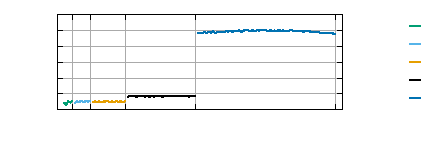
\includegraphics{TestModuloInverseComputation2}}%
    \gplfronttext
  \end{picture}%
\endgroup
%
	\vspace{-3mm}
	\caption{Runtimes for computing multiplicative inverses.}%
	\label{fig:ExtEuclideanSpeed}%
	\vspace{-4mm}
\end{figure}


\textbf{Conclusion.} The micro benchmarks proof that using the multiplicative inverse makes AN coding well competitive, which is why \emph{Continuous} and \emph{Reencoding} perform so good at SSB. %The inverse need not be stored in meta data and can be computed once per operator. 

%\subsection{Summary}
%Regarding decoding and detection runtime, original AN coding performs poorly against other codings like Hamming and XOR checksums. In contrast, the micro benchmarks proof In contrast to Hamming and checksum, AN coding further allows (i) to easy adjust the detection capabilities using the parameter $A$ and (ii) to directly work on the encoded data representation during query processing, which we efficiently used for on-the-fly error detection. 

%\section{Discussion}
%\label{sec:Discussion}

%Before we conclude the paper, we discuss related and future work in this section. Here, we limit our discussion to database-specific related work. A broader discussion is given in Appendix~\ref{sec:RelatedWork_Hardware}.

%\subsection{Related Work}
\section{Related Work}
\label{sec:RelatedWork}

A few years ago, Boehm et al.~\cite{DBLP:journals/pvldb/BohmLF11} already pointed out the lack of data management techniques dealing with an increasing number of bit flips in main memory as an increasingly relevant source. In~\cite{DBLP:conf/srds/PittelliG86,DBLP:journals/tocs/PittelliG89}, the combination of TMR and database systems was investigated. The most recent database-specific work of Kolditz et al. \cite{DBLP:conf/damon/KolditzKSHL14} hardens index structures like B-Trees using various techniques for online error detection. They have shown that slightly increasing data redundancy at the right places by incorporating context knowledge increases error detection significantly. \emph{AHEAD} can be extended by their work (cf. \Cref{sec:StorageConcept,sec:Implementation}). Furthermore, checksums are usually utilized to check for data integrity. For instance, HDFS computes a checksum of each data block and stores it in separate, hidden files~\cite{DBLP:conf/mss/ShvachkoKRC10}. Whenever a client fetches a data block, it verifies the retrieved data using the associated checksum~\cite{DBLP:conf/mss/ShvachkoKRC10}, but this is only done for disk blocks leaving in-memory data vulnerable. %We are not aware of any work which includes continuous soft error detection in query processing.

Moreover, AN coding has also been used for software-based fault tolerance~\cite{DBLP:conf/hase/HoffmannUDSLS14,DBLP:phd/de/Schiffel2011,ulbrich2012eliminating}. For instance, the work of Schiffel~\cite{DBLP:phd/de/Schiffel2011} allows to encode existing software binaries or to add encoding at compile time, where not all variables' states need to be known in advance. However, in her work she only describes encoding integers of size \(|\mathbb{D}|\in\{1, 8, 16, 32\}\) bits and pointers, where the encoded values are always 64 bits large. Furthermore, protecting processors by AN coding was also suggested in~\cite{forin1989vital}.

%\subsection{Future Work}
%\section{Future Work}
%
%We are fully aware that our \emph{AHEAD} approach is just a starting point and does not cover everything. From our point of view, the following next steps are necessary:
%
%\textbf{Optimization and Extension:} In Section~\ref{sec:SSBEval} we show that our current storage overhead is suboptimal. Bit-level data compression as in~\cite{Willhalm:2009:SUF:1687627.1687671,willhalm2013vectorizing} could be one solution. While data hardening and lightweight compression~\cite{DBLP:conf/sigmod/AbadiMF06,DBLP:conf/edbt/DammeHHL17,vectorizedMonetDB} are orthogonal to each other, their interplay is very important to keep the overall memory footprint of data as low as possible. With hardening, compression gains even more significance, since it can reduce the newly introduced storage overhead. However, combining both may be challenging and has to be investigated in detail. Furthermore, \emph{AHEAD} cannot detect errors in logic operations, whereas these are frequently used in database systems, e.g., in novel column storage layouts like BitWeaving~\cite{Li:2013:BFS:2463676.2465322} and ByteSlice~\cite{Feng:2015:BPE:2723372.2747642}. This domain must be considered separately, whereby \emph{AHEAD} can serve as the basis. Further extensions to \emph{AHEAD} could be (1) the use of code word accumulators to do detection every \(n\)th code word, trading accuracy against performance, or (2) hardening of database meta data and block or string data. Moreover, our \emph{AHEAD} approach should be investigated in multi-threaded environments for scalability reasons. 
%
%
%\textbf{Error Correction:} So far, we were concerned with the continuous detection of bit flips during query processing. Next, continuous error correction should be considered so that detected bit flips are corrected during query processing. With \emph{AHEAD}, we are able detect bit flips on value granularity and can find out where the error occurred. Based on that, specific correction techniques can be developed and integrated in the query processing. For example, if we detect a faulty code word in the inputs of an operator, we can retransmit it, possibly several times, to correct errors induced during transmission. If we get a valid code word, processing can continue with this correct code word. If we get an invalid code word, we can assume that bits are flipped in main memory and then we require an appropriate techniques for error correction. For that, correcting errors in the memory requires data redundancy in any case. Here, classical RAID-techniques or techniques from the network coding domain may be interesting. 
%
%\textbf{Cross-Layer Approach:} AHEAD is primarily a software approach. Another interesting research direction would examine the interplay of hardware and software protection mechanisms. In particular, what should be done in hardware and what should be done in software. Form our point of view, \emph{AHEAD} could serve as foundation for such a novel research direction~\cite{DBLP:books/daglib/0037372}.
%
%


%\begin{compactitem}
%	\item conduct research on error correction based on AHEAD
%	\begin{compactitem}
%		\item[\(\rightarrow\)] compensation queries
%		\item[\(\rightarrow\)] network coding approaches like linear combinations
%	\end{compactitem}
%	\item investigate interplay between
%	\begin{compactitem}
%		\item techniques on the different software and hardware layers for bit flip resilient systems
%		\begin{compactitem}
%			\item[\(\rightarrow\)] use compiler techniques like SWIFT to harden database meta data
%			\item[\(\rightarrow\)] compute the SDC probabilities when using AN coding on ECC main memory
%		\end{compactitem}
%		\item various compression techniques or storage layouts and AN coding
%		\begin{compactitem}
%			\item[\(\rightarrow\)] compression e.g. 4-wise null suppression or run length encoding
%			\item[\(\rightarrow\)] storage layouts e.g. ByteSlice and BitWeaving
%		\end{compactitem}
%	\end{compactitem}
%	\item examine other software coding approaches or completely different techniques as alternatives to AN coding
%	\begin{compactitem}
%		\item[\(\rightarrow\)] checksums for strings or block data
%	\end{compactitem}
%	\item integrate (hardened) dictionaries into AHEAD
%	\item compute more super \(A\)s
%	\item integrate AHEAD approach into an existing DBMS
%	\item implement vectorization on other SIMD architectures
%	\begin{compactitem}
%		\item[\(\rightarrow\)] AVX2, AVX512, ARM neon
%	\end{compactitem}
%	\item in-depth evaluation against other software coding approaches, i.e. use general-purpose frameworks to protect the baseline and compare against Continuous Detection
%	\begin{compactitem}
%		\item[\(\rightarrow\)] e.g. SWIFT, ELZAR, HAFT
%	\end{compactitem}
%\end{compactitem}

% !TeX encoding = UTF-8
% !TeX root = sigmod2018.tex
% !TeX spellcheck = en_US
\section{Conclusion and Outlook}
\label{sec:Conclusion}

Future hardware becomes less reliable in total and scaling up todays hardware-based protection introduces too much overhead~~\cite{DBLP:journals/micro/Borkar05,DBLP:conf/dac/HenkelBDGNSTW13,DBLP:books/daglib/0037372,DBLP:journals/it/ShafiqueABCCDEH15}. Therefore, a shift towards mitigating these reliability issues at higher layers, rather than only dealing with these issues in hardware was initiated~\cite{DBLP:conf/dac/HenkelBDGNSTW13,DBLP:books/daglib/0037372,DBLP:journals/it/ShafiqueABCCDEH15}. However, traditional general-purpose software-based protection techniques mainly rely on dual modular redundancy (DMR) to detect errors~\cite{goloubeva2006software,oh2002error,DBLP:conf/cgo/ReisCVRA05,DBLP:books/daglib/0037372}. For database systems, DMR introduces high overhead, because all data has to be duplicated and every query is executed redundantly including a result comparison as the final step. To overcome these drawbacks, we have presented our novel \emph{adaptable and on-the-fly \textbf{error detection} approach} called \emph{AHEAD}. With our approach, we achieve the following properties: (1) \emph{AHEAD} detects (i) errors (multi\=bit flips) that modify data stored in main memory or transmit over an interconnect and (ii) errors induced during computations, (2) \emph{AHEAD} provides configurable error detection capabilities to be able to adapt to different error models at run-time, and (3) \emph{AHEAD} drastically reduces the overhead compared to DMR and errors are continuously detected at query processing. Thus, \emph{AHEAD} is the first comprehensive database-specific approach to tackle the challenge of resilient query processing on unreliable hardware. As next, the following steps have to be done: 

\textbf{Optimization and Extension:} In Section~\ref{sec:SSBEval} we show that our current storage overhead is suboptimal. Bit-level data compression as in~\cite{Willhalm:2009:SUF:1687627.1687671,willhalm2013vectorizing} could be one solution. While data hardening and lightweight compression~\cite{DBLP:conf/sigmod/AbadiMF06,DBLP:conf/edbt/DammeHHL17} are orthogonal to each other, their interplay is very important to keep the overall memory footprint of data as low as possible. With hardening, compression gains even more significance, since it can reduce the newly introduced storage overhead. However, combining both may be challenging and has to be investigated in detail. Furthermore, \emph{AHEAD} cannot detect errors in logic operations, whereas these are frequently used in database systems, e.g., in novel column storage layouts like BitWeaving~\cite{Li:2013:BFS:2463676.2465322} and ByteSlice~\cite{Feng:2015:BPE:2723372.2747642}. This domain must be considered separately, for this, \emph{AHEAD} can serve as the basis. Further extensions of \emph{AHEAD} could be (1) the use of code word accumulators to do detection every \(n\)th code word, trading accuracy against performance, or (2) hardening of database meta data and block or string data. %Moreover, our \emph{AHEAD} approach should be investigated in multi-threaded environments for more scalability considerations. 


\textbf{Error Correction:} So far, we were concerned with the continuous detection of bit flips during query processing. Next, continuous error correction should be considered so that detected bit flips are corrected during query processing. With \emph{AHEAD}, we are able detect bit flips on value granularity and can find out where the error occurred. Based on that, specific correction techniques can be developed and integrated in the query processing. For example, if we detect a faulty code word in the inputs of an operator, we can retransmit it, possibly several times, to correct errors induced during transmission. If we get a valid code word, processing can continue with this correct code word. If we get an invalid code word, we can assume that bits are flipped in main memory and then we require an appropriate technique for error correction. For that, correcting errors in the memory requires data redundancy in any case. %Here, classical RAID-techniques or techniques from the network coding domain may be interesting to consult. 

\textbf{Cross-Layer Approach:} AHEAD is primarily a software approach. Another interesting research direction would examine the interplay of hardware and software protection mechanisms. In particular it should be scrutinized what should be done in hardware and what should be done in software. From our point of view, \emph{AHEAD} could serve as foundation for such a novel research direction~\cite{DBLP:books/daglib/0037372}.



\section*{Acknowledgments}
This work is partly funded by the German Research Foundation (DFG) within the Cluster of Excellence “Center for Advancing Electronics Dresden” (Resilience Path). Parts of the evaluation hardware were generously provided by the Dresden GPU Center of Excellence. We also thank the anonymous reviewers for their constructive feedback to improve this paper.


\clearpage

\begin{figure*}[t!]%
	\centering
	\footnotesize
	\graphicspath{{results/ssb/report/}}
	\begin{subfigure}[t]{6.5in}
		% GNUPLOT: LaTeX picture with Postscript
\begingroup
  \makeatletter
  \providecommand\color[2][]{%
    \GenericError{(gnuplot) \space\space\space\@spaces}{%
      Package color not loaded in conjunction with
      terminal option `colourtext'%
    }{See the gnuplot documentation for explanation.%
    }{Either use 'blacktext' in gnuplot or load the package
      color.sty in LaTeX.}%
    \renewcommand\color[2][]{}%
  }%
  \providecommand\includegraphics[2][]{%
    \GenericError{(gnuplot) \space\space\space\@spaces}{%
      Package graphicx or graphics not loaded%
    }{See the gnuplot documentation for explanation.%
    }{The gnuplot epslatex terminal needs graphicx.sty or graphics.sty.}%
    \renewcommand\includegraphics[2][]{}%
  }%
  \providecommand\rotatebox[2]{#2}%
  \@ifundefined{ifGPcolor}{%
    \newif\ifGPcolor
    \GPcolortrue
  }{}%
  \@ifundefined{ifGPblacktext}{%
    \newif\ifGPblacktext
    \GPblacktexttrue
  }{}%
  % define a \g@addto@macro without @ in the name:
  \let\gplgaddtomacro\g@addto@macro
  % define empty templates for all commands taking text:
  \gdef\gplbacktext{}%
  \gdef\gplfronttext{}%
  \makeatother
  \ifGPblacktext
    % no textcolor at all
    \def\colorrgb#1{}%
    \def\colorgray#1{}%
  \else
    % gray or color?
    \ifGPcolor
      \def\colorrgb#1{\color[rgb]{#1}}%
      \def\colorgray#1{\color[gray]{#1}}%
      \expandafter\def\csname LTw\endcsname{\color{white}}%
      \expandafter\def\csname LTb\endcsname{\color{black}}%
      \expandafter\def\csname LTa\endcsname{\color{black}}%
      \expandafter\def\csname LT0\endcsname{\color[rgb]{1,0,0}}%
      \expandafter\def\csname LT1\endcsname{\color[rgb]{0,1,0}}%
      \expandafter\def\csname LT2\endcsname{\color[rgb]{0,0,1}}%
      \expandafter\def\csname LT3\endcsname{\color[rgb]{1,0,1}}%
      \expandafter\def\csname LT4\endcsname{\color[rgb]{0,1,1}}%
      \expandafter\def\csname LT5\endcsname{\color[rgb]{1,1,0}}%
      \expandafter\def\csname LT6\endcsname{\color[rgb]{0,0,0}}%
      \expandafter\def\csname LT7\endcsname{\color[rgb]{1,0.3,0}}%
      \expandafter\def\csname LT8\endcsname{\color[rgb]{0.5,0.5,0.5}}%
    \else
      % gray
      \def\colorrgb#1{\color{black}}%
      \def\colorgray#1{\color[gray]{#1}}%
      \expandafter\def\csname LTw\endcsname{\color{white}}%
      \expandafter\def\csname LTb\endcsname{\color{black}}%
      \expandafter\def\csname LTa\endcsname{\color{black}}%
      \expandafter\def\csname LT0\endcsname{\color{black}}%
      \expandafter\def\csname LT1\endcsname{\color{black}}%
      \expandafter\def\csname LT2\endcsname{\color{black}}%
      \expandafter\def\csname LT3\endcsname{\color{black}}%
      \expandafter\def\csname LT4\endcsname{\color{black}}%
      \expandafter\def\csname LT5\endcsname{\color{black}}%
      \expandafter\def\csname LT6\endcsname{\color{black}}%
      \expandafter\def\csname LT7\endcsname{\color{black}}%
      \expandafter\def\csname LT8\endcsname{\color{black}}%
    \fi
  \fi
    \setlength{\unitlength}{0.0500bp}%
    \ifx\gptboxheight\undefined%
      \newlength{\gptboxheight}%
      \newlength{\gptboxwidth}%
      \newsavebox{\gptboxtext}%
    \fi%
    \setlength{\fboxrule}{0.5pt}%
    \setlength{\fboxsep}{1pt}%
\begin{picture}(9360.00,1440.00)%
    \gplgaddtomacro\gplbacktext{%
      \csname LTb\endcsname%
      \put(412,297){\makebox(0,0)[r]{\strut{}$0$}}%
      \csname LTb\endcsname%
      \put(412,466){\makebox(0,0)[r]{\strut{}$0.5$}}%
      \csname LTb\endcsname%
      \put(412,635){\makebox(0,0)[r]{\strut{}$1$}}%
      \csname LTb\endcsname%
      \put(412,804){\makebox(0,0)[r]{\strut{}$1.5$}}%
      \csname LTb\endcsname%
      \put(412,973){\makebox(0,0)[r]{\strut{}$2$}}%
      \csname LTb\endcsname%
      \put(412,1142){\makebox(0,0)[r]{\strut{}$2.5$}}%
      \csname LTb\endcsname%
      \put(412,1311){\makebox(0,0)[r]{\strut{}$3$}}%
      \csname LTb\endcsname%
      \put(1052,124){\makebox(0,0){\strut{}Q1.1}}%
      \csname LTb\endcsname%
      \put(1579,124){\makebox(0,0){\strut{}Q1.2}}%
      \csname LTb\endcsname%
      \put(2106,124){\makebox(0,0){\strut{}Q1.3}}%
      \csname LTb\endcsname%
      \put(2633,124){\makebox(0,0){\strut{}Q2.1}}%
      \csname LTb\endcsname%
      \put(3160,124){\makebox(0,0){\strut{}Q2.2}}%
      \csname LTb\endcsname%
      \put(3687,124){\makebox(0,0){\strut{}Q2.3}}%
      \csname LTb\endcsname%
      \put(4214,124){\makebox(0,0){\strut{}Q3.1}}%
      \csname LTb\endcsname%
      \put(4740,124){\makebox(0,0){\strut{}Q3.2}}%
      \csname LTb\endcsname%
      \put(5267,124){\makebox(0,0){\strut{}Q3.3}}%
      \csname LTb\endcsname%
      \put(5794,124){\makebox(0,0){\strut{}Q3.4}}%
      \csname LTb\endcsname%
      \put(6321,124){\makebox(0,0){\strut{}Q4.1}}%
      \csname LTb\endcsname%
      \put(6848,124){\makebox(0,0){\strut{}Q4.2}}%
      \csname LTb\endcsname%
      \put(7375,124){\makebox(0,0){\strut{}Q4.3}}%
    }%
    \gplgaddtomacro\gplfronttext{%
      \csname LTb\endcsname%
      \put(94,804){\rotatebox{-270}{\makebox(0,0){\strut{}Relative Runtime}}}%
      \csname LTb\endcsname%
      \put(8990,1174){\makebox(0,0)[r]{\strut{}Unprotected}}%
      \csname LTb\endcsname%
      \put(8990,1026){\makebox(0,0)[r]{\strut{}DMR}}%
      \csname LTb\endcsname%
      \put(8990,878){\makebox(0,0)[r]{\strut{}Early}}%
      \csname LTb\endcsname%
      \put(8990,730){\makebox(0,0)[r]{\strut{}Late}}%
      \csname LTb\endcsname%
      \put(8990,582){\makebox(0,0)[r]{\strut{}Continuous}}%
      \csname LTb\endcsname%
      \put(8990,434){\makebox(0,0)[r]{\strut{}Reencoding}}%
    }%
    \gplbacktext
    \put(0,0){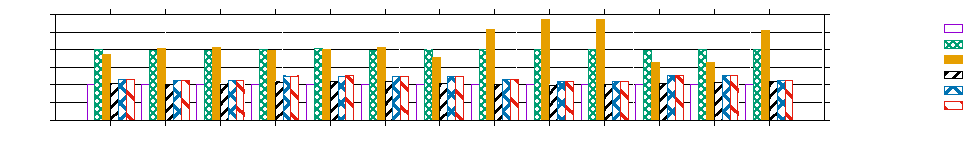
\includegraphics{norm-all_scalar}}%
    \gplfronttext
  \end{picture}%
\endgroup

	\end{subfigure}
	\vspace{-0.3cm}
	\caption{Relative SSB runtimes for scalar execution (average over all scale factors).}%
	\label{fig:eval:runtime:scalar}%
	\vspace{-0.4cm}
\end{figure*}

\printbibliography

\appendix
\section{SSB Scalar Runtime Performance}
\label{sec:SSBEval:scalar}

Figure~\ref{fig:eval:runtime:scalar} shows the relative scalar runtimes for all 13 SSB queries as averages over all 10 scale factors and 10 runs each. The \textbf{Unprotected} variant is the baseline. \textbf{DMR} shows the expected \(100\%\) runtime overhead, whereas \textbf{Early} has very high overheads between 64\% and 185\%, where the main overhead results from the slow \(\Delta\) operator which decodes all encoded columns. The overhead of \textbf{Late Detection} is always below 10\%. \textbf{Continuous} and \textbf{Reencoding} runtimes show overheads between 10\% and 27\%.

\section{Protection Techniques}
\label{sec:RelatedWork_Hardware}

\textbf{Hardware-based protection} can be done on three layers~\cite{DBLP:books/daglib/0037372}: (i) transistor, (ii) circuit, and (iii) architectural. On the \emph{transistor layer}, several techniques have been proposed to harden transistors against radiation events like alpha particles or neutron strikes~\cite{itoh1980single,kohara1990mechanism}. For example, thick polyamide can be used for alpha particle protection~\cite{itoh1980single,kohara1990mechanism}. However, this technique cannot be utilized for neutron strikes~\cite{DBLP:books/daglib/0037372}. In general, techniques at this layer have in common that the protection results in adopted fabrication processes using specialized materials~\cite{itoh1980single,kohara1990mechanism,DBLP:books/daglib/0037372}. Therefore, these techniques are very effective, but they produce (i) substantial overhead in terms of area and cost, and (ii) immense validation and verification costs. 

At the \emph{circuit layer}, redundant circuits and error detection/correc\-tion circuits are prominent examples~\cite{dell1997white,ernst2004razor,Kim:2007:MET:1331699.1331719,DBLP:books/daglib/0037372}. For instance, the RAZOR approach introduces shadow flip flops in the pipeline to recover from errors in logic gates~\cite{ernst2004razor}. Memories and caches are usually protected using error correcting codes (ECC) or parity techniques. Current ECC memories are based on Hamming using a (72,64) code, meaning that 64 bits of data are enhanced with 8 bits of parity allowing single error correction and double error detection. However, this is not sufficient to address multi-bit flips. To tackle multi-bit flips advanced ECC schemes have to be used. Examples are (i) IBM's Chipkill approach, wich computes the parity bits from different memory words and even separate DIMMs instead of physically adjacent bits~\cite{dell1997white}, and (ii) \cite{Kim:2007:MET:1331699.1331719}, which shows that other ECC codes like BCH-codes~\cite{moon2005error} can be realized in hardware to be able to correct e.g., 8-bit flips and detect 9-bit flips for 64 bits of data. However, this increases the number of transistors in hardware and consequently impacts the energy demand, the overhead growing quickly as the code strength is increased~\cite{Kim:2007:MET:1331699.1331719}. Additionally, reading and computing the enhanced ECC bits can be a performance bottleneck during read operations~\cite{Kim:2007:MET:1331699.1331719}. To mitigate \emph{disturbance errors} at this layer, hardware vendors improve inter-cell isolation, but this is challenging due to ever-decreasing feature sizes and higher densities~\cite{DBLP:conf/isca/KimDKFLLWLM14,DBLP:conf/date/Mutlu17}. 

At the \emph{architectural layer}, the protection is based upon the redundant execution either in space (using duplicated hardware units) or in time (using the same hardware multiple times for redundant execution and comparing the results). Dual Modular Redundancy (DMR) and Triple Modular Redundancy (TMR) are traditional approaches. Generally, these techniques lead to an increased power usage which may potentially increase the temperature~\cite{DBLP:books/daglib/0037372}. Increased temperatures lead to higher soft error rate and increased aging~\cite{DBLP:books/daglib/0037372}. To lower these effects, multi-/manycore architectures provide soft error tolerance through the availability of a high number of cores. Idle cores can now be exploited to provide redundancy either at the hardware level (using redundant instructions or redundant threads) or operating system level (using redundant thread processes). For example, the Simultaneous Redundant Threading (SRT) approach~\cite{DBLP:conf/isca/ReinhardtM00} adapts the concept of Simultaneous Multithreading (SMT)~\cite{DBLP:conf/isca/TullsenEL95}. SMT was proposed to improve performance via executing program codes of different applications in a simultaneous multithreaded fashion on multiple functional units inside a given processor. In contrast to that, SRT executes two redundant threads of the same application on multiple functional units and then performs the output comparison. 

To summarize, hardware-based protection techniques are usually very effective, but they also have major drawbacks in terms of (i) high area overhead leading at the same time to more power overhead and (ii) performance penalties. Furthermore, the high verification/validation costs make the reliable hardware design and development very expensive and time consuming~\cite{DBLP:books/daglib/0037372}. To overcome these non-negligible drawbacks, a rich set of software-based techniques has evolved. 

\textbf{Classical software-based protection} techniques are~\cite{goloubeva2006software,DBLP:books/daglib/0037372}: (i) N-version programming, (ii) code redundancy, (iii) control flow checking, and (iv) checkpoint recovery. For instance, N-version programming~\cite{DBLP:journals/tse/Avizienis85} is based on implementing multiple program versions of the same specification which reduces the probability of identical errors occurring in two or more versions. State-of-the-art redundancy-based techniques are Error Detection using Duplicated Instructions (EDDI)~\cite{oh2002error} and Software Implemented Fault Tolerance (SWIFT)~\cite{DBLP:conf/cgo/ReisCVRA05}. Both provide software reliability by duplicating instructions, and inserting comparison and checking instructions. However, these techniques incur significant performance overheads~\cite{oh2002error,DBLP:conf/cgo/ReisCVRA05}. %but various extensions and optimizations have been proposed over the last years~\cite{DBLP:conf/cd/ChenNV16,DBLP:conf/emsoft/DobelHE12, DBLP:journals/taco/ReisCVRAM05,kuvaiskii2016elzar}. 

%Moreover, AN coding has also been used for software-based fault tolerance~\cite{DBLP:conf/hase/HoffmannUDSLS14,DBLP:phd/de/Schiffel2011,ulbrich2012eliminating}. For instance, the work of Schiffel~\cite{DBLP:phd/de/Schiffel2011} allows to encode existing software binaries or to add encoding at compile time, where not all variables' states need to be known in advance. However, in her work she only describes encoding integers of size \(|\mathbb{D}|\in\{1, 8, 16, 32\}\) bits and pointers, where the encoded values are always 64 bits large. Furthermore, protecting processors by AN coding was also suggested in~\cite{forin1989vital}.

%\input{01-appendix.tex}
%\input{02-appendix-interplay.tex}
%We computed the SDC probabilities of the AN codes with \(|A| \leq 16\), whereby the 
%We now show how we computed the SDC probabilities of the AN codes with \(|A| \leq 16\). For the following, we reuse the definitions from Section~\ref{sec:ANCoding}.

 % Runtime AN-Coding exact, AN-Coding qMC M {Runtime, max.rel.err}, Hamming {Runtime, max.rel.err}
% M = 0.01*2^k
\begin{table}%[!hb]
	\centering
	\sisetup{
		round-mode=places,
		round-precision=0
	}
	\renewcommand{\arraystretch}{1.2}
	\begin{tabular}{@{}lrrrrrrrr@{}}
		\toprule
		& \multicolumn{3}{c}{exact} & \multicolumn{2}{c}{$\sigma_{\text{grid,1D},4\cdot\mathrm{GPU}}$} & 
		\\[-\aboverulesep]
		\arrayrulecolor[gray]{0.5}\cmidrule(lr){2-4}\cmidrule(lr){5-6}\arrayrulecolor{black}
		$k$ & $t_{\mathrm{CPU}}$ & $t_{1\cdot\mathrm{GPU}}$ & $t_{4\cdot\mathrm{GPU}}$ & $t_M$ & $\Delta_M$ & $M$\\
		\midrule
		8  & \SI{6.786}{\milli\second{}}   & \SI{0.658}{\milli\second{}}   & \SI{3.022}{\milli\second{}}  & \SI{5.856}{\milli\second{}}   & \num[round-precision=4]{0.02321} & 101\\
16 & \SI{375.533}{\milli\second{}} & \SI{129.728}{\milli\second{}} & \SI{40.707}{\milli\second{}} & \SI{10.516}{\milli\second{}}  & \num[round-precision=4]{0.00305} & 1001\\
24 & \SI{382.133}{\minute{}}       & \SI{99.485}{\minute{}}        & \SI{27.019}{\minute{}}       & \SI{353.865}{\milli\second{}} & \num[round-precision=4]{0.00527} & 1001\\
32 & --                            & --                            & --                           & \SI{4.889}{\minute{}}         & --                               & 1001\\

		\bottomrule
	\end{tabular}
	\caption{Computing the distance distributions of AN codes for \(A=61\). Average values after 5 runs.
	% TODO[include] on the Bull HPC-Cluster at TU Dresden.
CPU: 2$\times$E5-2680 v3 Haswell 12-core \SI[round-precision=2]{2.50}{GHz}, gcc5.3, OpenMP 4.0. GPU: NVIDIA Tesla K80, CUDA 7.5}
	\label{tab:runtimes}
	\vspace{-3em}
\end{table}

\section{Computing The SDC Probability}
\label{appendix:SDCProbability}

There is plenty of work on evaluating the probability of undetected errors for linear block codes\footnote{For linear codes, the linear combination (\emph{exclusive} OR) of two valid code words is \emph{always} also a valid code word.} and Hamming code in particular~\cite{KAUR19941141,Wolf1982,moon2005error}. For AN codes, this has only been done for 8- and 16-bit data and \(A\)s up to 8 and 16 bits~\cite{DBLP:conf/hase/HoffmannUDSLS14,coredExperiments}. However, this is insufficient for the database domain, because \begin{inparaenum} \item possibly all data bit widths between 1 and 64 bits are to be supported~\cite{willhalm2013vectorizing}, and \item larger \(A\)s may be required for future error models\end{inparaenum}. To overcome that, we developed a practical methodology for determining the probability of SDC for non-systematic, non-linear\footnote{In non-linear codes, the linearity property is not always satisfied.} coding schemes in general and independent of a specific error model~\cite{kolditz2018}. For this, we use the following definitions: A code \(\mathbb{C}\) (EDC/ECC) is defined by the triplet $(n, k, d_\text{min})$, were $n=|\mathbb{C}|$ is the code word width, $k$ is the data width, and $d_\text{min}$ is the minimum Hamming distance between any of the code's valid code words. Further, $b$ denotes the number of flipped bits. For AN coding, the definitions from Section~\ref{sec:ErrorCoding} further apply.
 


%Moreover, we assume no specific probability for the occurrence of any error patterns and only compute conditional likelihoods. We assume this, because, to the best of our knowledge, there is no error model for future hardware technologies, which would provide us with specific probabilities of the number and rate of bit flips per data unit (byte, word, etc.), or probabilities for certain error patterns. If there is one available, we could well integrate it.

\begin{figure}[t]
	\centering
	{
		\graphicspath{{gnuplot/}}
		% GNUPLOT: LaTeX picture with Postscript
\begingroup
  \makeatletter
  \providecommand\color[2][]{%
    \GenericError{(gnuplot) \space\space\space\@spaces}{%
      Package color not loaded in conjunction with
      terminal option `colourtext'%
    }{See the gnuplot documentation for explanation.%
    }{Either use 'blacktext' in gnuplot or load the package
      color.sty in LaTeX.}%
    \renewcommand\color[2][]{}%
  }%
  \providecommand\includegraphics[2][]{%
    \GenericError{(gnuplot) \space\space\space\@spaces}{%
      Package graphicx or graphics not loaded%
    }{See the gnuplot documentation for explanation.%
    }{The gnuplot epslatex terminal needs graphicx.sty or graphics.sty.}%
    \renewcommand\includegraphics[2][]{}%
  }%
  \providecommand\rotatebox[2]{#2}%
  \@ifundefined{ifGPcolor}{%
    \newif\ifGPcolor
    \GPcolortrue
  }{}%
  \@ifundefined{ifGPblacktext}{%
    \newif\ifGPblacktext
    \GPblacktexttrue
  }{}%
  % define a \g@addto@macro without @ in the name:
  \let\gplgaddtomacro\g@addto@macro
  % define empty templates for all commands taking text:
  \gdef\gplbacktext{}%
  \gdef\gplfronttext{}%
  \makeatother
  \ifGPblacktext
    % no textcolor at all
    \def\colorrgb#1{}%
    \def\colorgray#1{}%
  \else
    % gray or color?
    \ifGPcolor
      \def\colorrgb#1{\color[rgb]{#1}}%
      \def\colorgray#1{\color[gray]{#1}}%
      \expandafter\def\csname LTw\endcsname{\color{white}}%
      \expandafter\def\csname LTb\endcsname{\color{black}}%
      \expandafter\def\csname LTa\endcsname{\color{black}}%
      \expandafter\def\csname LT0\endcsname{\color[rgb]{1,0,0}}%
      \expandafter\def\csname LT1\endcsname{\color[rgb]{0,1,0}}%
      \expandafter\def\csname LT2\endcsname{\color[rgb]{0,0,1}}%
      \expandafter\def\csname LT3\endcsname{\color[rgb]{1,0,1}}%
      \expandafter\def\csname LT4\endcsname{\color[rgb]{0,1,1}}%
      \expandafter\def\csname LT5\endcsname{\color[rgb]{1,1,0}}%
      \expandafter\def\csname LT6\endcsname{\color[rgb]{0,0,0}}%
      \expandafter\def\csname LT7\endcsname{\color[rgb]{1,0.3,0}}%
      \expandafter\def\csname LT8\endcsname{\color[rgb]{0.5,0.5,0.5}}%
    \else
      % gray
      \def\colorrgb#1{\color{black}}%
      \def\colorgray#1{\color[gray]{#1}}%
      \expandafter\def\csname LTw\endcsname{\color{white}}%
      \expandafter\def\csname LTb\endcsname{\color{black}}%
      \expandafter\def\csname LTa\endcsname{\color{black}}%
      \expandafter\def\csname LT0\endcsname{\color{black}}%
      \expandafter\def\csname LT1\endcsname{\color{black}}%
      \expandafter\def\csname LT2\endcsname{\color{black}}%
      \expandafter\def\csname LT3\endcsname{\color{black}}%
      \expandafter\def\csname LT4\endcsname{\color{black}}%
      \expandafter\def\csname LT5\endcsname{\color{black}}%
      \expandafter\def\csname LT6\endcsname{\color{black}}%
      \expandafter\def\csname LT7\endcsname{\color{black}}%
      \expandafter\def\csname LT8\endcsname{\color{black}}%
    \fi
  \fi
    \setlength{\unitlength}{0.0500bp}%
    \ifx\gptboxheight\undefined%
      \newlength{\gptboxheight}%
      \newlength{\gptboxwidth}%
      \newsavebox{\gptboxtext}%
    \fi%
    \setlength{\fboxrule}{0.5pt}%
    \setlength{\fboxsep}{1pt}%
\begin{picture}(4740.00,2880.00)%
    \gplgaddtomacro\gplbacktext{%
      \colorrgb{0.27,0.27,0.27}%
      \put(455,558){\makebox(0,0)[r]{\strut{}\scriptsize{$10^{-5}$}}}%
      \colorrgb{0.27,0.27,0.27}%
      \put(455,948){\makebox(0,0)[r]{\strut{}\scriptsize{$10^{-4}$}}}%
      \colorrgb{0.27,0.27,0.27}%
      \put(455,1338){\makebox(0,0)[r]{\strut{}\scriptsize{$10^{-3}$}}}%
      \colorrgb{0.27,0.27,0.27}%
      \put(455,1727){\makebox(0,0)[r]{\strut{}\scriptsize{$10^{-2}$}}}%
      \colorrgb{0.27,0.27,0.27}%
      \put(455,2117){\makebox(0,0)[r]{\strut{}\scriptsize{$10^{-1}$}}}%
      \colorrgb{0.27,0.27,0.27}%
      \put(455,2507){\makebox(0,0)[r]{\strut{}\scriptsize{$10^{0}$}}}%
      \colorrgb{0.27,0.27,0.27}%
      \put(612,317){\makebox(0,0){\strut{}\scriptsize{$10^{1}$}}}%
      \colorrgb{0.27,0.27,0.27}%
      \put(1159,317){\makebox(0,0){\strut{}\scriptsize{$10^{2}$}}}%
      \colorrgb{0.27,0.27,0.27}%
      \put(1706,317){\makebox(0,0){\strut{}\scriptsize{$10^{3}$}}}%
      \colorrgb{0.27,0.27,0.27}%
      \put(2254,317){\makebox(0,0){\strut{}\scriptsize{$10^{4}$}}}%
      \colorrgb{0.27,0.27,0.27}%
      \put(2801,317){\makebox(0,0){\strut{}\scriptsize{$10^{5}$}}}%
      \colorrgb{0.27,0.27,0.27}%
      \put(2958,558){\makebox(0,0)[l]{\strut{}\scriptsize{$10^{-3}$}}}%
      \colorrgb{0.27,0.27,0.27}%
      \put(2958,836){\makebox(0,0)[l]{\strut{}\scriptsize{$10^{-2}$}}}%
      \colorrgb{0.27,0.27,0.27}%
      \put(2958,1115){\makebox(0,0)[l]{\strut{}\scriptsize{$10^{-1}$}}}%
      \colorrgb{0.27,0.27,0.27}%
      \put(2958,1393){\makebox(0,0)[l]{\strut{}\scriptsize{$10^{0}$}}}%
      \colorrgb{0.27,0.27,0.27}%
      \put(2958,1672){\makebox(0,0)[l]{\strut{}\scriptsize{$10^{1}$}}}%
      \colorrgb{0.27,0.27,0.27}%
      \put(2958,1950){\makebox(0,0)[l]{\strut{}\scriptsize{$10^{2}$}}}%
      \colorrgb{0.27,0.27,0.27}%
      \put(2958,2229){\makebox(0,0)[l]{\strut{}\scriptsize{$10^{3}$}}}%
      \colorrgb{0.27,0.27,0.27}%
      \put(2958,2507){\makebox(0,0)[l]{\strut{}\scriptsize{$10^{4}$}}}%
    }%
    \gplgaddtomacro\gplfronttext{%
      \csname LTb\endcsname%
      \put(56,1532){\rotatebox{-270}{\makebox(0,0){\strut{}$\bm{\Delta}$}}}%
      \csname LTb\endcsname%
      \put(3305,1532){\rotatebox{-270}{\makebox(0,0){\strut{}$t$ in s}}}%
      \csname LTb\endcsname%
      \put(1706,38){\makebox(0,0){\strut{}$M$}}%
      \csname LTb\endcsname%
      \put(1706,2786){\makebox(0,0){\strut{}$k=24,\, A=61$}}%
      \csname LTb\endcsname%
      \put(4053,2595){\makebox(0,0)[r]{\strut{}$\frac{1}{\sqrt{M}}$}}%
      \csname LTb\endcsname%
      \put(4053,2316){\makebox(0,0)[r]{\strut{}$\frac{\log(M)}{M}$}}%
      \csname LTb\endcsname%
      \put(4053,2037){\makebox(0,0)[r]{\strut{}$t_{\text{exact}}$}}%
      \csname LTb\endcsname%
      \put(4053,1758){\makebox(0,0)[r]{\strut{}$t_{\text{pseudo}}$}}%
      \csname LTb\endcsname%
      \put(4053,1479){\makebox(0,0)[r]{\strut{}$t_{\text{quasi}}$}}%
      \csname LTb\endcsname%
      \put(4053,1200){\makebox(0,0)[r]{\strut{}$t_{\text{grid}}$}}%
      \csname LTb\endcsname%
      \put(4053,921){\makebox(0,0)[r]{\strut{}$\bm{\Delta}_{\text{pseudo}}$}}%
      \csname LTb\endcsname%
      \put(4053,642){\makebox(0,0)[r]{\strut{}$\bm{\Delta}_{\text{quasi}}$}}%
      \csname LTb\endcsname%
      \put(4053,363){\makebox(0,0)[r]{\strut{}$\bm{\Delta}_{\text{grid}}$}}%
    }%
    \gplbacktext
    \put(0,0){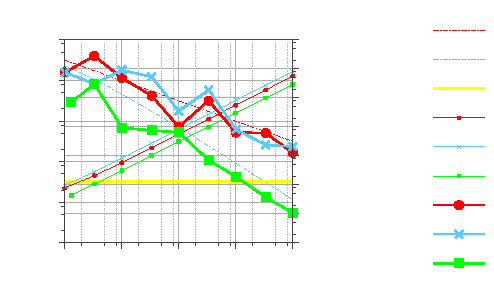
\includegraphics{converge}}%
    \gplfronttext
  \end{picture}%
\endgroup

	}
	\vspace{-2em}
	\caption{Convergence of maximum relative error $\Delta$ and run-time \(t\) according to the number of iterations $M$.}
	\label{fig:convergence}
	\vspace{-0.4cm}
\end{figure} 

Conceptually, we model the space of all \emph{valid} code words as an undirected, fully connected, weighted graph, where the code words are the vertices. Each valid code word is connected with every other valid one and the edge weights denote the \emph{Hamming distance} $d_H$ between the two code words. Thus, we only concentrate on the \emph{transitions} originating from valid code words to other valid ones, \emph{regardless of the coding}. Then, computing SDC probabilities requires two steps. First, we build a histogram over all transition weights, by which we get the numbers $c_b$ of undetectable $b$-bit flips:
\begin{Definition}
For a given code, $c_b$ denotes the number of transitions of weight \(b\) between valid code words.
\end{Definition}
The set \(\left\{c_b | b \in \left\{1,\dots,k\right\}\right\}\) is called \emph{weight distribution}. For AN coding, $c^A_b$ represents the count for a given \(A\). Second, we relate each $c_b$ to the respective total number of possible $b$-bit flips $\binom{n}{b}$.
Consequently, there can be $2^k \cdot \binom{n}{b}$ $b$-bit flips in all valid code words. This number includes all transitions from any \emph{valid} codeword to any other \emph{possible} code word. By that, when computing the weight distribution, we also have to count the transitions modeled in the graph twice (i.e., for each direction), because with a single error pattern we can make a transition in both direction. In total, this results in the SDC probability for $b$-bit flips, which we denote as:
\begin{equation}
p_b  = \frac{c_b}{2^k \cdot \binom{n}{b}}
\label{eq:sdc}
\end{equation}

Now, the challenge is to obtain \(c_b\) in an efficient manner. For non-linear codes like AN coding, \(c_b\) must be \emph{counted} in a brute force manner to the best of our knowledge. For AN coding, the convolution of the multiplication cannot be described in a way which allows simplifications. We use the following function to describe the naive approach:
\begin{equation}
	\delta_b (x, y) = \begin{cases}
		1,&\mathrm{if}\ {d_H(x,y)=b}, \\
		0,&\mathrm{if}\ {d_H(x,y)\neq b,}
	\end{cases}
	\qquad0\le b\le n\,.\nonumber
	\label{eq:delta}
\end{equation}
Then, we can compute the distance distribution as
\begin{equation}
	c_b = \sum_{\alpha\in\mathbb{C}} \sum_{\beta\in\mathbb{C}} \delta(\alpha, \beta)\,.
	\label{eq:naivecount}
\end{equation}
The complexity of Equation~(\ref{eq:naivecount}) is $\mathcal{O}(4^k)$, i.e. with each additional data bit, there are four times as many distances. In practice, it is half as much due to the symmetry (only one edge is computed and then counted twice). For parameter optimization, this might be run many thousands of times. Especially, for AN coding each odd \(A\) must be examined again for each data width \(|\mathbb{D}_\Theta|\) and with each additional bit, the number of candidates doubles. We call this naive approach \emph{exact}, as it examines all code words. For AN coding, Table~\ref{tab:runtimes} shows runtimes for the exact computation of the weight distribution for a single \(A\) using a single CPU, a single GPU, or a small cluster of 4 GPUs.




To mitigate the complexity, we use a sampling\=based approach, which approximates the weight distribution by comparing only a subset of all code words. Here, the main problem is the \emph{distribution} function for choosing the subset of code words. We investigated three different distributions: pseudo\=random (\(\sigma_\text{pseudo}\)), quasi\=random (\(\sigma_\text{quasi}\)), and grid-point (\(\sigma_\text{grid}\)). Note that \(\sigma_\text{pseudo}\) is prone to clustering, while \(\sigma_\text{quasi}\) fills the space more uniformly. The probabilistic error of Monte\=Carlo (pseudo\=random) is known to be $\mathcal{O}(\nicefrac{1}{\sqrt{M}})$ and for quasi\=Monte\=Carlo it is $\mathcal{O}(\nicefrac{(\log M)^q}{M})$ with number of dimensions $q$ and number of iterations $M$~\cite{montecarlo}. The grid\=point approach chooses regularly aligned samples, given by $\sigma_\text{grid}(r) = \nicefrac{(2^k\cdot r)}{M}$. If $M=2^k$, then the grid sampling yields the correct result, while random numbers still miss the solution due to collisions and gaps. Figure~\ref{fig:convergence} shows a comparison between the three distributions of convergence and runtime for the case \(k=24\) and \(A=61 \Rightarrow n=30\) and includes the theoretic Monte\=Carlo error boundaries. Pseudo- and quasi\=random numbers were generated with the cuRAND library. The 1D grid approximation outperforms the random distributions in virtually all cases, yielding smaller error \(\Delta\) and lower runtime \(t\). It is, furthermore, directly influenced by the value of \(M\), and we found that \emph{odd} values lead to much smaller errors than even ones.

\begin{algorithm}[t]
\caption{AN code distance distribution -- basic algorithm}
\label{alg:ancoding}
\begin{algorithmic}[1]
\Require $k\ge2$
\Require Value $A>0$, $n=k+h$, $h=\lceil\log_2(A)\rceil$
\Require Initial distance distribution $c^A_b=0,\,b=0,\ldots,n$
\Ensure Distance distribution $c^A$ of code $C_A$
\For{$\alpha=0,\ldots,(2^k-1)$} \Comment{outer loop is parallelized on GPU[s]} \label{alg:ancoding:1}
\For{$\beta=\sigma_\text{grid}(r),~r=0,\dots,M$}  \Comment{inner loop is processed by each thread} \label{alg:ancoding:2}
 \State $b \gets d_H( A\alpha, A\beta )$
 \State $c^A_b \gets c^A_b + 1$  \label{alg:ancoding:4}
\EndFor
\EndFor
\State \Return $c^A$
\end{algorithmic}
\end{algorithm}

Algorithm~\ref{alg:ancoding} shows the 1D grid approach for enumerating the weight distribution of an AN code. For GPU clusters, we distribute the outer loop evenly across the GPUs. When symmetry is exploited in line~\ref{alg:ancoding:2}, the workload size of each GPU is computed by:
\begin{equation}
	\lceil 2^k\omega_{i+1} \rceil - \lceil 2^k\omega_{i} \rceil,~w_i=1-\sqrt{1-\nicefrac{i}{N}},~0\le i<N \mbox{=\#GPUs}
	\label{eq:workload}
\end{equation}
$\omega_i$ is the solution of $\int_{i}^{i+1}1{-}x\,\mathrm{d}x=\nicefrac{1}{N}$ for equal work size areas. The maximal relative error of the estimation $\hat{c}^A_b$ is given by $\Delta = \max_{b>0} \frac{\mid c^A_b - \hat{c}^A_b \mid}{c^A_b}$ ($b=0$ is omitted due to $c^A_0=2^k$).

Algorithm~\ref{alg:ancoding} can be parallelized on GPUs, since the Hamming distances of two code
 words can be computed independently. We use CUDA C/C++ for programming Nvidia GPUs. As registers of GPUs are 32\=bit wide, the multi\=GPU implementation uses 32\=bit integers as long as the array elements in a thread do not overflow. From Equation~\ref{eq:sdc} follows $\max_b c_b^A\le\max_b 2^k\binom{n}{b}=2^k\binom{n}{n/2}$ and the upper bound for using 32\=bit integers is:
\[
c^A_{b,\mathrm{thread}}\le\frac{2^k\binom{n}{n/2}}{\mathrm{threads}}<2^{32}~.
\]
%It should be possible to use $\frac{2^k\binom{k}{k/2}}{\mathrm{threads}}$ as a lower bound, since higher values of $A$ make the distance distribution wider and flatter to keep the total sum equal to $4^k$. If \num4 GPUs are used with \num{64000} threads each, the 64\=bit implementation is used when $k\ge27$.
The GPU uses 64 bits for the global array, so the highest data bit width for the GPU algorithm is $k=33$. The range for each GPU is between $\lceil 2^k\omega_{i} \rceil$ and $\lceil 2^k\omega_{i+1} \rceil$ from Equation~\ref{eq:workload}. We use thread\=local arrays and one global array to avoid memory contention. Since local array indexing is dynamic and non\=uniform, it cannot be stored into the fast registers, as they are not addressable at run\=time. Hence, the local array is stored in local memory, which is L1 cached thread\=private global memory. To get scalable and flexible kernels, the outer loop strides by the size of a CUDA grid (threads per block $\times$ blocks per grid). The kernel is called with \lstinline{blocks}=$32\cdot\mathrm{numberOfMultiprocessors}$ and $128$ threads per block. After the local histogram is filled, atomic operations are used to add the values to the global distance distribution. The respective runtimes are shown in Table~\ref{tab:runtimes} on the right half. More details can be found in~\cite{kolditz2018}.



%Finally, we list all smallest super \(A\)s per bit flip weight which we computed until now in Table~\ref{tab:optimalAsComplete} and more super \(A\)s will be calculated. All up-to-date information will be available on our github project web page. 
%Note that super \(A\)s are not always increasing with larger \(|\mathbb{D}|\).

\begin{table}%
	\footnotesize
	\setlength{\tabcolsep}{0.7em} % for the horizontal padding
	\begin{tabular}{r|rrrrrrr}
		\toprule
		\multirow{2}{*}{\(|\mathbb{D}_\Theta|\)} & \multicolumn{6}{c}{minimal detectable bit flip weight} \\
		   & \multicolumn{1}{c}{1} & \multicolumn{1}{c}{2} & \multicolumn{1}{c}{3} & \multicolumn{1}{c}{4} & \multicolumn{1}{c}{5} & \multicolumn{1}{c}{6} & \multicolumn{1}{c}{7} \\
		\midrule
		 1 & \textbf{3}/2 &  \textbf{7}/3 &            15/4 &    \textbf{31}/5 &              63/6 &   \textbf{127}/7 &    255/8  \\
		 2 & \textbf{3}/2 & \textbf{13}/4 &   \textbf{53}/6 &            213/8 &   \textbf{853}/10 &          3285/12 & 13141/14  \\
		 3 & \textbf{3}/2 & \textbf{29}/5 &            45/6 &   \textbf{467}/9 &           1837/11 & \textbf{7349}/13 & 23733/15 \\
		 4 & \textbf{3}/2 &          27/5 &   \textbf{89}/7 &           933/10 &           6777/13 &         31385/15 \\
		 5 & \textbf{3}/2 & \textbf{29}/5 &           117/7 &           933/10 &           7085/13 &         31373/15 \\
		 6 & \textbf{3}/2 & \textbf{29}/5 &  \textbf{233}/8 &          1899/11 &           7837/13 &         62739/16 \\
		 7 & \textbf{3}/2 & \textbf{29}/5 &           217/8 &          1803/11 & \textbf{13963}/14 &         55831/16 \\
		 8 & \textbf{3}/2 & \textbf{29}/5 &  \textbf{233}/8 &          1939/11 & \textbf{13963}/14 &         55831/16 \\
		 9 & \textbf{3}/2 & \textbf{29}/5 &           185/8 &          1939/11 &          15717/14 &         55831/16 \\
		10 & \textbf{3}/2 & \textbf{61}/6 &           185/8 & \textbf{3739}/12 &          27425/15 \\
		11 & \textbf{3}/2 & \textbf{61}/6 &           451/9 & \textbf{3739}/12 &          27425/15 \\
		12 & \textbf{3}/2 & \textbf{61}/6 &  \textbf{463}/9 &          3737/12 &          29925/15 \\
		13 & \textbf{3}/2 & \textbf{61}/6 &  \textbf{463}/9 &          3349/12 &          27825/15 \\
		14 & \textbf{3}/2 & \textbf{61}/6 &  \textbf{463}/9 &          6717/13 &          63877/16 \\
		15 & \textbf{3}/2 & \textbf{61}/6 &  \textbf{463}/9 &          7785/13 &          63877/16 \\
		16 & \textbf{3}/2 & \textbf{61}/6 &  \textbf{463}/9 &          7785/13 &          63877/16 \\
		17 & \textbf{3}/2 & \textbf{61}/6 &           393/9 &          7785/13 &          63859/16 \\
		18 & \textbf{3}/2 & \textbf{61}/6 & \textbf{947}/10 &          7785/13 &          63859/16 \\
		... & ... \\
		28 & \textbf{3}/2 &         111/7 &          951/10 &         29685/15 \\
		29 & \textbf{3}/2 &         111/7 &          835/10 &        *29685/15 \\
		30 & \textbf{3}/2 &         125/7 &          835/10 &        *31693/15 \\
		31 & \textbf{3}/2 &         125/7 & \textbf{881}/10 &        *32211/15 \\
		32 & \textbf{3}/2 &         125/7 & \textbf{881}/10 &        *32417/15 \\
		\bottomrule
	\end{tabular}
	\caption{Smallest super \(A\)s per minimal detectable bit flip weight in the form \(A/|A|\). \textbf{Bold} numbers are prime. * obtained through grid approximation.}
	\label{tab:optimalAsComplete}
	\vspace{-3em}
\end{table}

\section{Github}
\label{sec:GitHub}
Finally, we would like to point out our project \emph{BRICS-DB} on GitHub\footnote{https://brics-db.github.io/} where our prototypical \emph{AHEAD} implementation is available, as well as our GPU implementation for computing distance distributions (SDC probability). We also provide the full table for all smallest super \(A\)s per bit flip weight which we computed until now. More super \(A\)s will be calculated and all updated information will be provided on github. Table~\ref{tab:optimalAsComplete} shows an excerpt of the current table of super \(A\)s.

%Actually, we computed all super \(A\)s for all \(1\leq|A|\leq16\) until time of submission.


\end{document}
